% ---------- Titelblad Masterproef Faculteit Wetenschappen -----------
% Dit document is opgesteld voor compilatie met pdflatex.  Indien je
% wilt compileren met latex naar dvi/ps, dien je de figuren naar
% (e)ps-formaat om te zetten.
%                           -- december 2012
% -------------------------------------------------------------------
\RequirePackage{fix-cm}
\documentclass[12pt,a4paper,oneside]{book}



% --------------------- In te laden pakketten -----------------------
% Deze kan je eventueel toevoegen aan de pakketten die je al inlaadt
% als je dit titelblad integreert met de rest van thesis.
% -------------------------------------------------------------------
\usepackage{graphicx,xcolor,textpos}
\usepackage{helvet}
\usepackage{amsmath}
\usepackage{bm}
\usepackage{amsfonts}
\usepackage{empheq} 
\usepackage{enumitem}
%\usepackage{apacite}
\usepackage{babel} 
\usepackage{apalike}
\usepackage{algorithm}
\usepackage[noend]{algpseudocode}
\usepackage{booktabs}
\usepackage{parskip}
\usepackage{caption}

% Use Heuristica Font
\usepackage{tocloft}



% -------------------- Pagina-instellingen --------------------------
% Indien je deze wijzigt, zal het titelblad ook wijzigen.  Dit dien je
% dan manueel aan te passen.
% --------------------------------------------------------------------

\topmargin -10mm
\textwidth 160truemm
\textheight 240truemm
\oddsidemargin 0mm
\evensidemargin 0mm

% ------------------- textpos-instellingen ---------------------------
% Enkele andere instellingen voor het voorblad.
% --------------------------------------------------------------------

\definecolor{green}{RGB}{172,196,0}
\definecolor{bluetitle}{RGB}{29,141,176}
\definecolor{blueaff}{RGB}{0,0,128}
\definecolor{blueline}{RGB}{82,189,236}
\setlength{\TPHorizModule}{1mm}
\setlength{\TPVertModule}{1mm}


%--------------------- Nieuwe Commando's -----------------------------
\newtheorem{Definition}{Definition}
\newtheorem{Lemma}{Lemma}
\newtheorem{Properties}{Properties}
\newtheorem{Theorem}{Theorem}
\DeclareMathOperator{\sgn}{sgn}
\newenvironment{proof}{\paragraph{Proof:}}{\hfill$\square$}
\makeatletter
\def\BState{\State\hskip-\ALG@thistlm}
\makeatother
\DeclareMathOperator{\Tr}{Tr}

\def\signed #1{{\leavevmode\unskip\nobreak\hfil\penalty50\hskip2em
  \hbox{}\nobreak\hfil(#1)%
  \parfillskip=0pt \finalhyphendemerits=0 \endgraf}}

\newsavebox\mybox
\newenvironment{aquote}[1]
  {\savebox\mybox{#1}\begin{quote}}
  {\signed{\usebox\mybox}\end{quote}}
  
\renewcommand*\oldstylenums[1]{\textosf{#1}}
\addtolength{\cftsecnumwidth}{10pt} 


\begin{document}

\frontmatter

% ---------------------- Voorblad ------------------------------------
% Vergeet niet de tekst aan te passen:
% - Titel en, indien van toepassing, ondertitel
%          voor eventuele formules in de titel of ondertitel
%          gebruik je  \form{$...$}
% - Je naam
% - Je (co)promotor, begeleider (indien van toepassing)
% - Je opleiding
% - Het academiejaar
% --------------------------------------------------------------------
\thispagestyle{empty}
\newcommand{\form}[1]{\scalebox{1.087}{\boldmath{#1}}}
\sffamily
%
\begin{textblock}{191}(-24,-11)
\colorbox{green}{\hspace{123mm}\ \parbox[c][18truemm]{68mm}{\textcolor{white}{FACULTY OF SCIENCE}}}
\end{textblock}
%
\begin{textblock}{70}(-18,-19)
\textblockcolour{}
\includegraphics*[height=19.8truemm]{LogoKULeuven}
\end{textblock}
%
\begin{textblock}{160}(-6,63)
\textblockcolour{}
\vspace{-\parskip}
\flushleft
\fontsize{40}{42}\selectfont \textcolor{bluetitle}{\form{Machine Learning}} \\ \fontsize{40}{42}\selectfont \textcolor{bluetitle} {\form{In Quantitative Finance}}
\texttt{\fontsize{20}{22}\selectfont \form{A kernel of truth}}
\end{textblock}
%
%\begin{textblock}{79}(50,103)
%\textblockcolour{}
%\vspace{-\parskip}
%\flushleft
%\fbox{\parbox{79mm}{De achtergrond kan wit blijven of je kan een afbeelding invoegen (maximum hoogte 10 cm, breedte variabel, denk aan auteursrechten\ldots). GEEN logo's (je kan binnenin de masterproef logo's gebruiken, maar niet op de voor- of achterpagina). \textit{Verwijder deze tekstkader.}}}
%\end{textblock}
%
\begin{textblock}{160}(8,153)
\textblockcolour{}
\vspace{-\parskip}
\flushright
\fontsize{14}{16}\selectfont \textbf{Lennert VAN DER SCHRAELEN}
\end{textblock}
%
\begin{textblock}{70}(-6,191)
\textblockcolour{}
\vspace{-\parskip}
\flushleft
Supervisor: Prof. W. Schoutens\\[-2pt]
\textcolor{blueaff}{Department Mathematics, \textsl{}}
\textcolor{blueaff}{Statistics \& Risk Management \textsl{}}\\[5pt]
%Co-promotor: \textsl{(facultatief)}\\[-2pt]
%\textcolor{blueaff}{Affiliatie \textsl{(facultatief)}}\\[5pt]
Mentor: \textsl{S. Reyners}\\[-2pt]
\textcolor{blueaff}{Department Mathematics, \textsl{}}
\textcolor{blueaff}{Statistics \& Risk Management \textsl{}}\\[5pt]
\end{textblock}
%
\begin{textblock}{160}(8,191)
\textblockcolour{}
\vspace{-\parskip}
\flushright
Thesis presented in\\[4.5pt]
fulfillment of the requirements\\[4.5pt]
for the degree of Master of Science\\[4.5pt]
in Mathematics\\
\end{textblock}
%
\begin{textblock}{160}(8,232)
\textblockcolour{}
\vspace{-\parskip}
\flushright
Academic year 2019-2020
\end{textblock}
%
\begin{textblock}{191}(-24,248)
{\color{blueline}\rule{550pt}{5.5pt}}
\end{textblock}
%
\vfill
\newpage

% Als je het titelblad wil integreren met de rest van je thesis,
% kan je hieronder verder.
% ----------------------- Eerste pagina's -------------------------
% Hier kan je inhoudsopgave, voorwoord en dergelijke kwijt.
% -----------------------------------------------------------------
\rmfamily
\setcounter{page}{0}
%\pagenumbering{roman}


\newpage

© Copyright by KU Leuven

Without written permission of the promotors and the authors it is forbidden to reproduce or adapt in any form or by any means any part of this publication. Requests for obtaining the right to reproduce or utilize parts of this publication should be addressed to KU Leuven, Faculteit Wetenschappen, Geel Huis, Kasteelpark Arenberg 11 bus 2100, 3001 Leuven (Heverlee), Telephone +32 16 32 14 01.

A written permission of the promotor is also required to use the methods, products, schematics and programs described in this work for industrial or commercial use, and for submitting this publication in scientific contests.

\newpage

\tableofcontents

\newpage

\section{Acknowledgement}

I wish to show my gratitude to my supervisor, professor Schoutens Wim, and my mentor, Reyners Sofie, proposing this interesting subject and providing a pleasant working atmosphere by giving support when necessary.
\\
\\
I wish to show my respect to professor Quaegebeur Johan, who learned me to understand mathematics.
\\
\\
Next, I wish to thank my mother, Jannsens Jo, my father, Van der Schraelen Danny,  and my brother, Van der Schraelen Arne, since they are just always there for me. 
\\
\\
I would like to pay my special regards to my classmates of Mathematics, which are responsible for an unforgettable $5$ years. Special thanks are given to Andries Hannah, Bouwen Ben, Dompas Annabel, Gielis Simon, Nevelsteen Stephanie, Op de Beeck Nicolas, Schruers Dorien, Torfs Sofie, Van den Borne Bram, Vanmechelen Pieter, Van Kruijsdijck Gregory, Vermeiren Stephanie and Wolfs Jasper.
\\
\\
Finally, I wish to show my gratitude to Ardenoy Arno, Olbrechts Ruben and Stuyck Raf. I hope we stay lifelong friends despite the different paths we may take.
\\
\\
\\
\\
\\
\\
\\
\begin{aquote}{As I Lay Dying: `The sound of truth'}
But what wisdom is there within us \\
To live based on the feeling of our hearts \\
How many times has instinct let us down \\
Never to be thought through, never to be questioned \\
\end{aquote}

\newpage

\section{Symbols and Notation}

We try to use the notation in a consistent way. Matrices are capitalized and vectors are in bold type. Notice that financial parameters are also often capitalized. We denote a quantity corresponding with a test set with a superscript asterix. Before using a non-prominent notation for the first time in the text, we always repeat its definition.  
\\
\\
\begin{tabular}{ll}
$\setminus$ &   Left matrix divide: $X = A \setminus B$ is the solution of $A X = B$  \\
$:=$ &  Equality which is a definition   \\
$\circ$ & Element-wise multiplication \\
$\sim$ &   Is distributed as \\
$(x)^+$ & The maximum of $x$ and zero \\
$\tilde{A}$ & A small modification (on $A$) \\
$||.||_{\mathcal{H}}$ &  RKHS norm   \\
$<.,.>_{\mathcal{H}}$ &  RKHS inner product  \\
$|A|$ & Determinant of $A$ \\
$\bm{y}^t$ &   the transpose of $\bm{y}$ \\
$\nabla$ & Gradient   \\
$\bigotimes$ &  Kronecker product  \\
$B$ & Banach space \\
$\delta_x$ & evaluation functional   \\
$\mathbb{E}$ &  Expectation  \\
$\bm{f}$ & Vector of latent function values $\bm{f} = (\bm{f}(\bm{x}_1), \ldots,\bm{f}( \bm{x}_n))^t$ (GPR)   \\
$\bm{f}^{\ast}$ &    Posterior prediction  \\
$\gamma$ & Gain or learning rate \\
$\Gamma$ & For brevity \\
$\mathcal{GP}$ & Gaussian process   \\
$H$ & Barrier \\
$\mathcal{H}$& Hilbert space (Functional Analysis)  Model structure (Bayesian analysis)  \\
$I_n$ &  $n \times n$ Identity matrix  \\
$\kappa$ & The speed of mean reverting in the Heston model \\ 
$k$ &    kernel (GPR) log strike price (finance) \\
$k_{\bm{x},\bm{z}}$ &    validation of kernel with input $\bm{x} , \bm{z}$\\
$K$ &  Gram matrix (GPR) strike price (financial) \\
$K(X,X) = K_{X,X}$ & $n \times n$ covariance (or Gram) matrix   \\
$K_{X,Z}$& $n \times m$ covariance (or Gram) matrix   \\
$\hat{K}_{X,X}$ &  Equals $\tilde{K}_{X,X} + \sigma^2 I_n$ \\
$KL$& Kullback-Leiber divergence    \\
$\mathcal{L}$ & Variational lower bound   \\
$\lambda_i$ &  $i$th Eigenvalue  \\ 
$\Lambda$ & For brevity (sparse GPR) \\
\end{tabular}

\begin{tabular}{ll}
$m$ &   Amount of inducing points \\
$\bm{m}$ &   Mean of the inducing points  \\
$n^{\ast}$ & amount of predictions \\
$n$ &   Amount of covariates in the model / which we want to predict \\
$\mathcal{N}(\mu, \sigma^2)$ &  Normal distribution with mean $\mu$ and variance $\sigma^2$ \\
$O(\cdot)$ &  Big oh notation   \\
$p(\bm{y}|\bm{x})$ &  The density of $\bm{y}$ given $\bm{x}$    \\
$q$ &  Dividend yield (finance) Approximate distribution (GPR) \\
$q_{s_T}(s)$ & Risk neutral density of log stock price at maturity \\
$q_{\bm{x}_i,\bm{x}_j}$ &    validation of the SoR approximation kernel with input $\bm{x}_i , \bm{x}_j$ \\
$Q$ & Risk-neutral pricing measure \\ 
$Q_{A,B} = K_{A,Z} K_{Z,Z}^{-1} K_{Z,B}$ &  For brevity (sparse GPR)\\
$\rho$ & Correlation parameter \\ 
$r$ &  Interest rate \\
$\mathbb{R}$ &  The real numbers  \\
$\sigma$ &  Volatility (finance) or noise variance (GPR)  \\
$\Sigma$ & Variance or for brevity (sparse GPR) \\
$S$ & Variance of the inducing points \\
$S_t$ & Price of the stock at time $t$    \\
$\theta$ & The vol-of-vol in het Heston model \\ 
$\bm{\theta}$ & Vector of Hyperparameters   \\
$\Theta$ & Parameter space \\
$t$ & Time  \\
$T$ & Maturity \\
$\Tr{(A)}$ &  Trace of A  \\
$\bm{u}$ &  Response vector for $Z$  \\
$\phi(\cdot)$ &  Feature map  \\
$\phi_{T}(\cdot)$ & Characteristic function of $q_{s_T}(s)$ \\ 
$\varphi(\cdot)$ & Eigenfunction  \\
$\bm{v}$ & (Eigen)vector \\ 
$\mathbb{V}$ &  Variance  \\
$v_t$ & Variance at time $t$ Heston model \\
$W$ & Sparse matrix    \\
$X$ &  design matrix containing the covariates \\
$X_t$ & stochastic process \\
$\mathcal{X}$ & Input space   \\
$\bm{y}$&   response vector for $X$\\
$(\Omega, \mathcal{F}, \mathcal{P})$ &  probability space  \\
$w$ & Weights f.e. for regression \\
$W_t$ &  A brownian motion  \\
$\bm{z}$ & Latent variables (sparse GPR), \\
& Samples from a normal distributed r.v.  \\
$Z$ & Parameters corresponding to the inducing values $\bm{u}$ (sparse GPR) \\
\end{tabular}

\mainmatter


\chapter{Abstract} 

This thesis is the continuation of \cite{de2018machine}, which is a paper written by De Spiegeleer Jan, Madan Dilip B, Reyners Sofie (my mentor) and Schoutens Wim (my supervisor). Both documents aim to deploy machine learning in the context of traditional quant problems. We focus on the fast pricing of derivatives using Gaussian Process Regression (GPR). Instead of executing time expensive calculations in order to price derivatives, we aim to train a model which we can consult achieving a speed-up. However, the price we have to pay for this speed-up is some loss in accuracy. 

We start with discussing the necessary financial knowledge concerning pricing derivatives. Thereafter, we give a short summary concerning the necessary mathematical pre-knowledge for understanding Gaussian Processes. Next, we discuss the basic algorithm for Gaussian process regression which time complexity for training and fitting is $O(n^3)$, $O(n^2)$ receptively. Subsequently, we try to modify/improve this algorithm obtaining a speed up for training and prediction and discuss when these new algorithms are suitable. We discuss different techniques which among other exploit the structure of the data, approximate our problem and/or uses advanced numerical methods. Some of these modifications achieve a considerable speed up considering training and/or predicting for a little loss accuracy. We also include a section discussing Bayesian and deep techniques for completeness. We end with a data study pricing different types of derivatives testing different GPR models.

We include a quite extensive appendix to which we often refer. Hence, it is recommended to print or to use two files so one can swap easily. A handy scheme giving an overview of the thesis can be found in section (\ref{summary}).

\chapter{Some Financial Pre-knowledge}

In this chapter, we discuss some options which we try to price in our data study. We also give a very short introduction to models which model the time evolution of a stock. 

\section{Options}\label{Options}

An option is a derivative which gives the investor the right, not an obligation, to buy or to sell a stock satisfying some predetermined terms and conditions. The buyer of a call option has the right to buy the stock from the seller at a certain time for the strike price ($K$). The buyer of a put option has the right to sell the stock from the seller at a certain time for the strike price. The two simplest types of options are European calls (EC) and puts (EP) which are also known as vanillas. These options need to be executed at the maturity ($T$). We denote with $Q$ the risk-neutral measure or pricing measure and with $+$ the maximum of a value and zero. We have the following expressions concerning their initial price

\begin{align}\label{price_vanillas}
&\text{Initial price EC}(K,T) :=  \exp{(-rT)} \mathbb{E}_{Q} [(S(T) - K)^{+} ] \\
&\text{Initial price EP}(K,T) :=  \exp{(-rT)} \mathbb{E}_{Q}[ (K - S(T))^{+}].
\end{align}

To obtain the pay-off, we just need to omit the expectation and the $\exp{(-rT)}$ (discounting) factor. We also try to price a down-and-out barrier put. If the option remains above a barrier $H$ during its lifetime $T$, it has the same structure as an European put with strike $K$. Its initial price is given by 

\begin{equation}
\text{Initial price DOBC} := \exp{(-rT)} \mathbb{E}_{Q}[(S_T-K)^{+} 1( \min\limits_{0 \leq t \leq T} S_t > H). 
\end{equation}

Notice that a lot of other barrier options are possible. We end with pricing American Options. For this type of option, the holder can exercise his rights during the entire life-time of the option and not only at the maturity. In the next section we try to model the time evolution of a stock. We begin with the well known Black and Scholes model. 

\section{The Black and Scholes Model}

We follow the approach of \cite{wimschoutensvg}, where the interested reader can find more details.  

\begin{Definition}[Geometric Brownian Motion]
Denote with $W_t$ a Brownian motion (see appendix section (\ref{Brownian_Motion})). Furthermore, denote with $S_t$ the price of the stock at time t, with $r$ the interest, $q$ the dividend yield and with $\sigma$ the volatility. The stochastic differential equation 

\begin{equation}
dS_t = S_t ((r-q) dt + \sigma dW_t),
\end{equation}
has an unique solution given by

\begin{equation}
S_t = S_0 \exp \left( \left((r-q) - \dfrac{\sigma^2}{2} \right) t + \sigma W_t \right)
\end{equation}
Which is called the geometric Brownian motion.
\end{Definition}

The expression of the geometric Brownian motion can be found using Ito's lemma. Notice that the logarithm of $S_t$ has a normal distribution and thus $S_t$ has a log normal distribution. By using $r$ and $q$ in this way, we are working in a risk neutral world.

Due to its simplicity, one can price many derivatives very easily and even closed form solutions for different options exist. One can even derive the Black and Scholes model as the limit of a tree model. For derivative pricing using tree models, see appendix section (\ref{appendix_tree}). 

However, the model is often too simple and has a lot of shortfalls. The log returns of empirical data typically do not behave according to a Normal distribution and show most of the time negative skewness and excess kurtosis. Hence, the Black-Scholes model can not model realistically extreme events. Notice that the model is continuous and shows no jumps, which is not the case in the financial market. Finally, the volatility parameter, which is the (only!) parameter, is assumed to be constant. However, the parameters of uncertainty change stochastically over time and are clustered in real life.

Hence, the Black and Scholes model not always suffices. In this thesis, we work with two well known models in the financial world which are more flexible and have better properties. 

\section{The Heston and Variance Gamma model}

In this section, we state some important results from \cite{heston1993closed} for the Heston model and from \cite{madan1998variance} and \cite{wimschoutensvg} for the Variance Gamma. 

\begin{Definition}[Heston stochastic volatility model]
Let us denote with $v_t>0$ the variance of the model at time $t$ and with $\sigma_0>0$ the standard deviation at time $0$. The paramater $\theta>0$ is the volatility of the volatility (vol-of-vol) and $\eta$ represents the long time variance of the model. The speed of the mean reverting of $v_t$ to $\eta$ is denoted with $\kappa>0$. The Brownian motion $\tilde{W}_t $ is correlated (parameter $-1<\rho<1$) with the Brownian motion $W_t $. The Heston stochastic volatility model is given by

\begin{equation}
\begin{aligned}
&dS_t = (r-q) dt + \sqrt{v_t} dW_t \\
&dv_t = \kappa (\eta - v_t) dt + \theta \sqrt{v_t} d \tilde{W}_t   \qquad v_0 = \sigma_0^2 \geq 0.
\end{aligned}
\end{equation}
\end{Definition}


Notice that we have included stochastic volatility in the model which was not the case in the Black and Scholes model. For equity markets, $\rho$ is typically negative since the volatility rises if the stock drops. Notice that this model does not include jumps, thus we discuss another model which does include jumps. 

Before we introduce the Variance-Gamma model, we define the Variance Gamma distribution and state the definition of a Variance-Gamma process.

\begin{Definition}[Variance Gamma distribution]
Suppose that the r.v. $X \sim \text{Gamma}(C,M)$ and $Y \sim \text{Gamma}(C,G)$ are independent. Then $\Gamma_1 \sim X-Y$ is Variance Gamma distributed i.e.  $\Gamma_1 \sim VG(C,G,M)$. 
\end{Definition}

One can also define the Variance Gamma distribution by
mixing a Normal and a Gamma distribution. 

\begin{Definition}[Variance-Gamma Process]
A stochastic process $X = \{ X_t, t \geq 0 \}$ is a Variance-Gamma Process with parameters $(C,G,M)$ on some probability space $(\Omega,\mathcal{F}, \mathcal{P})$, if

\begin{enumerate}
    \item $X_0 = 0$ a.s.
    \item $X$ has independent increments
    \item $X$ has stationary increments
    \item $X_{t+v} - X_t \sim VG(Cv,G,M)$.
\end{enumerate}
\end{Definition}

Notice the strong similarity with a Brownian motion, however, a VG process a jump process. By shifting the VG process in order to obtain a martingale, we find the following model. 


\begin{Definition}[Variance-Gamma model]
Denote with $X = \{X_t, t \geq 0 \}$  a Variance-Gamma process with parameters $(C,G,M)$ and write  

\begin{align*}
&\nu = 1/C \\ 
&\sigma^2 = 2C/(MG) \\ 
&\theta = C(G-M)/(MG) \\
&\omega = \nu^{-1} \log(1- \frac{1}{2} \sigma^2 \nu  - \theta \nu).
\end{align*}

The Variance-Gamma model of the stock price (risk-neutral) is given by
\begin{equation}
S_t = S_0 \exp \left( \left(r-q+w \right) t + \sigma X_t \right)
\end{equation}
\end{Definition}

Using these models one can price derivatives. For vanillas we use the Fast Fourrier Transform which can be found in the appendix section (\ref{Fast_Fourrier_transform}). For Barrier options we execute Monte-Carlo simulations (see appendix section (\ref{derivativesMCS})) and for American options a tree model (see appendix section\ref{appendix_tree}).



\chapter{Some Mathematical Pre-knowledge} 

Our main goal is to train a model using the training dataset and to make (fast) predictions. However, if we do not make any assumptions, every function which is consistent with the training data would be equally valid. We can for example only use one class of functions (for example only linear functions). However, it can be the case that this family is too simple and thus not sufficient. One also needs to pay attention for making the model to complex and thus for overfitting. 

We use an approach were we give a prior probability to every function. An higher probability is given to functions which we consider to be more likely, like smoother functions. In order to do so, one needs some knowledge about Bayesian - and functional analysis. 

\section{Bayesian Analysis}

In this section, we follow \cite{GPRbook} and \cite{camillagpr} and focus on Bayesian model selection. At the lowest level we consider $\bm{f}$ (the prediction function) and at the second level the hyperparameters $\bm{\theta}$ which control the distribution of $\bm{f}$. At the top level, we have a (discrete) set of possible model structures $\mathcal{H}_i$. We denote with $X$ the covariates and with $\bm{y}$ the response. From Bayes theorem (see appendix equation \ref{BayesTheorem} in the appendix), we find that the posterior of $\bm{f}$ at the lowest level is given by

\begin{equation}\label{Bayesian_analysis1}
p(f|\bm{y},X,\bm{\theta},\mathcal{H}_i) = \dfrac{p(\bm{y}|X,\bm{f},\mathcal{H}_i)p(\bm{f}|\bm{\theta},\mathcal{H}_i)}{p(\bm{y}|X,\bm{\theta},\mathcal{H}_i)}.
\end{equation}

Where $p(\bm{f}|\bm{\theta},\mathcal{H}_i)$ is the prior distribution of $\bm{f}$, $p(\bm{y}|X,\bm{f},\mathcal{H}_i)$ the likelihood function and $p(\bm{y}|X,\bm{\theta},\mathcal{H}_i)$ the normalising constant. If we condition on $\bm{f}$, we find that 

\begin{equation}\label{Bayesian_analysis2}
p(\bm{y}|X,\bm{\theta},\mathcal{H}_i) = \int p(\bm{y}|X,\bm{f},\mathcal{H}_i)p(\bm{f}|\bm{\theta},\mathcal{H}_i)d\bm{f}
\end{equation}

Subsequently, the posterior distribution of the hyperparameters
$\bm{\theta}$ is given by

\begin{equation}\label{Bayesian_analysis3}
p(\bm{\theta}|\bm{y},X,\mathcal{H}_i) = \dfrac{p(\bm{y}|X,\bm{\theta},\mathcal{H}_i)p(\bm{\theta}|\mathcal{H}_i)}{p(\bm{y}|X,\mathcal{H}_i)}.
\end{equation}

Where $p(\bm{\theta}|\mathcal{H}_i)$ is the prior distribution of $\bm{\theta}$, $p(\bm{y}|X,\bm{\theta},\mathcal{H}_i)$ the likelihood function and $p(\bm{y}|X,\mathcal{H}_i)$ the normalising constant. If we condition on $\bm{\theta}$, we find that 

\begin{equation}\label{Bayesian_analysis4}
p(\bm{y}|X,\mathcal{H}_i) = \int p(\bm{y}|X,\bm{\theta},\mathcal{H}_i)p(\bm{\theta}|\mathcal{H}_i)d\bm{\theta}
\end{equation}

At the top level, the posterior of the model is calculated

\begin{equation}\label{Bayesian_analysis5}
p(\mathcal{H}_i|\bm{y},X) = \dfrac{p(\bm{y}|X,\mathcal{H}_i)p(\mathcal{H}_i)}{p(\bm{y}|X)}.
\end{equation}

Depending on the model, some of the integrals can not be solved in an analytic way. Different ways to handle this problem can be found in the sections (\ref{section_bayesian_view}) and (\ref{section_hyperparameter_selection}). 
 

\section{Functional Analysis}\label{Functional_Analysis}

Although one can perfectly understand the machine learning techniques from a Bayesian or frequentist point of view, it is very interesting to approach our problems from another perspective. We briefly discuss some important items found in \cite{GPRbook} and \cite{sejdinovic2012rkhs}. For the Representer Theorem, we follow \cite{scholkopf2001generalized}.

\begin{Definition}[Banach space]
A Banach space is a complete normed space.
\end{Definition}

\begin{Definition}[Hilbert space]
A Hilbert space is a complete inner product space. In other words, it is a Banach space with inner product.
\end{Definition}

\begin{Definition}[Functional]
Let $B$ be a Banach space. Linear maps from $B$ to $\mathbb{C}$ are called functionals.
\end{Definition}

\begin{Definition}[Evaluation Functional]
Let $\mathcal{H}$ be a Hilbert space of functions $\mathcal{X} \rightarrow \mathbb{R}$, defined on a non-empty set $\mathcal{X}$. For a fixed $x \in \mathcal{X}$, the map $\delta_{\bm{x}} : \mathcal{H} \rightarrow \mathbb{R}: f \mapsto f(\bm{x})$ is called the evaluation functional at $\bm{x}$. 
\end{Definition}

Notice that evaluation functionals are always linear. However, they are not always continuous thus we define the motion of Reproducing Kernel Hilbert Space (RKHS), which behaves particularly well.

\begin{Definition}[Reproducing Kernel Hilbert Space]
A Hilbert space $\mathcal{H}$ of functions $\mathcal{X} \rightarrow \mathbb{R}$, defined on a non-empty set $\mathcal{X}$ is said to be a Reproducing Kernel Hilbert Space (RKHS) if $\delta_{\bm{x}}$ is continuous $\forall \bm{x} \in \mathcal{X}$.
\end{Definition}

Before we discuss what a RKHS have to do with kernels and machine learning, we give a rigorous definition of a kernel and a reproducing kernel.

\begin{Definition}[Kernel] \label{Functional_Kernel}
Let $\mathcal{X}$ be a non-empty set. The function $k: \mathcal{X} \times \mathcal{X} \rightarrow \mathbb{R}$ is said to be a kernel if there exists a real Hilbert space $\mathcal{H}$ and a map $\phi : \mathcal{X} \rightarrow \mathcal{H}$ such that $\forall \bm{x},\bm{x}' \in \mathcal{X}$,
\begin{equation}
k(\bm{x},\bm{x}') := \langle \phi(\bm{x}),\phi(\bm{x}') \rangle_{\mathcal{H}}.
\end{equation}
\end{Definition}

The map $\phi$ is called a feature map to the feature space $\mathcal{H}$.

\begin{Definition}[Reproducing kernel]
Let $\mathcal{H}$ be a Hilbert Space of $\mathbb{R}$-valued functions defined on a non-empty set $\mathcal{X}$. A function $k: \mathcal{X} \times \mathcal{X} \rightarrow \mathbb{R}$ is called a reproducing kernel of $\mathcal{H}$ if it satisfies 
\begin{itemize}
\item $\forall \bm{x} \in \mathcal{X}, k(\cdot,\bm{x}) \in \mathcal{X}$,
\item $\forall \bm{x} \in \mathcal{X}, \forall f \in \mathcal{H}, \langle f,k(\cdot,\bm{x})\rangle_{\mathcal{H}} := f(\bm{x}) \qquad$ (the reproducing property)
\end{itemize}
\end{Definition}

Notice that all reproducing kernels are kernels (take $\phi(\bm{x}) = k(\cdot,\bm{x})$). One can also prove that reproducing kernels, and thus kernels, are positive definite. Remember that every inner product is a positive definite function. 
We state two theorems from which we omit the doable proofs.

\begin{Theorem}[Uniqueness of the reproducing kernel] 
Let $\mathcal{H}$ be a Hilbert Space of $\mathbb{R}$-valued functions defined on a non-empty set $\mathcal{X}$. If a the reproducing kernel exists, it is unique.
\end{Theorem}

\begin{Theorem}[Existence of the reproducing kernel] 
$\mathcal{H}$ is an RKHS if and only if $\mathcal{H}$ has a reproducing kernel. 
\end{Theorem}

We denote the space of $\mathbb{R}$-valued functions defined on a non-empty set $\mathcal{X}$ with $\mathbb{R}^{\mathcal{X}}$. Now we are ready to state the famous theorem of Moore-Aronszajn.

\begin{Theorem}[Moore-Aronszajn theorem]
Let $\mathcal{X}$ be the non-empty input domain. Then for every positive definite function $k: \mathcal{X} \times \mathcal{X} \rightarrow \mathbb{R}$, there exists an unique RKHS $\mathcal{H} \subset \mathbb{R}^{\mathcal{X}}$ of $\mathbb{R}$-valued functions defined on a non-empty set $\mathcal{X}$  with reproducing kernel $k$.
\end{Theorem}

Hence, from Moore-Aronszajn, we find that every positive definite function is a reproducing kernel. We already knew that every kernel is positive definite and that every reproducing kernel is a kernel. Hence, these three notions are equivalent. 

From the fact that kernels are positive definite functions, we find the following theorem 

\begin{Theorem}[Sum and scaling of kernels]
If $k$, $k_1$ and $k_2$ are kernels  and $\alpha >0$ is a scalar, then $\alpha k$, $k_1 + k_2$ are kernels.
\end{Theorem}

Notice that the difference of kernels is not necessarily a kernel since it is not allowed to have that $k_1(\bm{x},\bm{x}) - k_2(\bm{x},\bm{x}) <0$. In this case, for the feature map $ \phi : \mathcal{X} \rightarrow \mathcal{H}$, the inproduct $\langle \phi(x),\phi(\bm{x}) \rangle_{\mathcal{H}}$ is smaller than zero which is not possible. For the product of kernels we find the following

\begin{Theorem}[Product of kernels]\label{Functional_Product}
Let $k_1$ and $k_2$ be kernels on $\mathcal{X}$ and $\mathcal{Z}$ respectively. We have that 
\begin{equation}\label{Functional_Product_first_eq}
k((\bm{x},\bm{z}),(\bm{x}',\bm{z}')) := k_1(\bm{x},\bm{x}')k_2(\bm{z},\bm{z}')
\end{equation}
is a kernel on $\mathcal{X} \times \mathcal{Y}$. In addition, if $k_1$ and $k_2$ are both kernels on $\mathcal{X}$, we find that 
\begin{equation}
k(\bm{x},\bm{x}') := k_1(\bm{x},\bm{x}')k_2(\bm{x},\bm{x}')
\end{equation}
is a kernel on $\mathcal{X}$.
\end{Theorem}

Hence, from the linear kernel $k_{lin} (\bm{x},\bm{x}') = \langle \bm{x},\bm{x}' \rangle$ and the previous two theorems we can construct polynomial kernels $ k_{\text{poly}}(\bm{x},\bm{x}') = (\langle \bm{x},\bm{x}' \rangle + c)^{m}$ , with $c>0$. Using Taylor series with non-negative co\"{e}fficients, we can construct the exponential kernel $ k_{\exp}(\bm{x},\bm{x}') = \exp(2\sigma \langle \bm{x},\bm{x}' \rangle)$ with $\sigma >0$. Due to its importance we derive how to construct the Gaussian kernel. Let $\phi : \mathbb{R}^d \rightarrow \mathbb{R} : \bm{x} \mapsto \exp(-\sigma ||\bm{x}||^2)$. If we define the ordinary inner product on $\mathbb{R}$, we know that $\mathbb{R}$ is a Hilbert space. Subsequently, using definition (\ref{Functional_Kernel}), we find that $\hat{k}(\bm{x},\bm{x}') = \phi(\bm{x}) \phi(\bm{x}') = \exp(-\sigma ||\bm{x}||^2) \exp(-\sigma ||\bm{x}'||^2)$ is a kernel on $\mathbb{R}^d$. Hence, using Theorem (\ref{Functional_Product}), we find the Gaussian kernel on $\mathbb{R}^d$ given by 

\begin{align}
k_{gauss}(\bm{x},\bm{x}') &= \hat{k}(\bm{x},\bm{x}') k_{\exp} (\bm{x},\bm{x}') \nonumber \\
 &= \exp{(-\sigma(||\bm{x}||^2 + ||\bm{x}'||^2 - 2 \langle \bm{x},\bm{x}' \rangle ))}  \nonumber \\
&= \exp{(-\sigma ||\bm{x}-\bm{x}'||^2)}.
\end{align}

Of course, we can classify our kernels. A stationary kernel is a function of $\bm{x} - \bm{x}'$, which is invariant to translations in the input space. Even stronger, if the kernel is only a function of $||\bm{x} - \bm{x}'||$, it is called isotropic and thus invariant to all rigid motions. An example is $k_{gauss}$. Note also that the Gaussian kernel on $\mathbb{R}^d$ is a product kernel since it can be written as a product of $d$ Gaussian kernels defined on a scalar input space.

%Denote with $k_c(\cdot,\cdot)$ an arbitrary kernel defined over a scalar input space. A kernel $k(\cdot,\cdot)$ is a tensor product kernel if we can write 

%\begin{equation}
%k(x,x') = \prod_{c=1}^{d} k_c(x_c,x'_c)),
%\end{equation}
%where $x_c$ and $x'_c$ are the c-th elements of $x$ respectively $x'$. 


Let us now consider one of the most important theorems of this section called the Representer Theorem, which generalises a large class of optimisation problems. 

\begin{Theorem}[Representer Theorem]\label{Functional_Representer}
Suppose we are given a nonempty set $\mathcal{X}$, a positive definite real valued kernel $k$ on $\mathcal{X} \times \mathcal{X}$, a training set $(\bm{x}_1,y_1), \cdots, (\bm{x}_n,y_n) \in \mathcal{X} \times \mathbb{R}$, a strictly monotonically increasing real-valued function $g$ on $[0, \infty [$, an arbitrary cost function $c : (\mathcal{X} \times \mathbb{R}^2)^n \rightarrow \mathbb{R} \cup \lbrace \infty \rbrace$ and a class of functions

\begin{equation}
\mathcal{F} = \left\{ f \in \mathbb{R}^{\mathcal{X}} | f(\cdot) = \sum\limits_{i=1}^{\infty} \beta_i k(\cdot,\bm{z}_i) , \beta_i \in \mathbb{R}, \bm{z}_i \in \mathcal{X} , || f|| < \infty \right\}.
\end{equation} 

Here, $||\cdot ||_{\mathcal{H}}$ is the norm in the RKHS $\mathcal{H}_k$ associated with kernel $k$, i.e. for any $\bm{z}_i \in \mathcal{X}, \beta_i \in \mathbb{R} (i \in \mathbb{N})$ we have that 

\begin{equation}
\left| \left| \sum\limits_{i=1}^{\infty} \beta_i k(\cdot,\bm{z}_i) \right|\right|_{\mathcal{H}}^2  = \sum\limits_{i,j=1}^{\infty} \beta_i \beta_j k(\bm{z}_i,\bm{z}_j).
\end{equation}

Then, any $f \in \mathcal{F}$ minimizing the regularized risk functional 

\begin{equation}\label{Functional_RegularizedRisk}
c((\bm{x}_1, y_1, f(\bm{x}_1)), \cdots , (\bm{x}_n, y_m, f(\bm{x}_n))) + g(||f||),
\end{equation}

admits a representation of the form 

\begin{equation}
f(\cdot) = \sum\limits_{i=1}^{n} \alpha_i k(\cdot,\bm{x}_i).
\end{equation}
\end{Theorem}

The first term of equation (\ref{Functional_RegularizedRisk}) is called the risk and is used for fitting the data. The second term is called the regularizer and serves as smoothness assumptions on $f$. We finish this section with some some notation and a very handy trick.

\begin{Definition}[Gram matrix]
Given a kernel $k$ and $\bm{x}_1,\cdots,\bm{x}_n \in \mathcal{X}$, the $n \times n$ matrix $K$ for which $K(i,j) = k(\bm{x}_i,\bm{x}_j)$ (with $1\leq i,j\leq n$) is called the Gram matrix of $k$ with respect to $\bm{x}_1, \ldots, \bm{x}_n$.
\end{Definition}

A Gram matrix corresponding to a kernel function as defined above is positive semi-definite. In order to obtain a non-linear version of an algorithm, one often replace $\bm{x}$ by $\phi(\bm{x})$. Thus we actually execute a mapping in a feature space. In other words, for $\bm{x}_i,\bm{x}_j \in \mathcal{X}$, $\langle \bm{x}_i, \bm{x}_j \rangle$ is replaced by $\langle \phi (\bm{x}_i) , \phi (\bm{x}_j) \rangle =k(\bm{x}_i,\bm{x}_j) = K(i,j)$. This called the Kernel Trick. From a computational point of view, by replacing $\langle \bm{x}_i, \bm{x}_j \rangle$ with $K(i,j)$, we turn a linear procedure into a non-linear procedure without adding much computation. 

Now we discuss Mercer's theorem which allows us to express a kernel $k$ in terms of eigenvalues and eigenfunctions. We denote with $T_k$  an integral operator defined as 

\begin{equation}
T_k (f) = \int k(\bm{x}, \bm{x}') f(\bm{x}') d \mu(\bm{x}')
\end{equation}

with $\mu$ a measure. A function $\varphi$ satisfying 

\begin{equation}
\int k(\bm{x},\bm{x}') \varphi(x) d \mu(\bm{x}) = \lambda \varphi(\bm{x}')
\end{equation}

is an eigenfunction of kernel $k$ with eigenvalue $\lambda$ with respect to the measure $\mu$. Now we are ready to state the following theorem.

\begin{Theorem}[Mercer's Theorem]\label{Functional_mercer}
Let $(\mathcal{X}, \mu)$ be a finite measure space and $k \in L_{\infty} (\mathcal{X}^2, \mu^2)$ be a kernel such that $T_k : L_2(\mathcal{X}, \mu) \rightarrow L_2(\mathcal{X}, \mu)$ is positive definite. Let $\varphi_i \in L_2(\mathcal{X},\mu)$ be the normalised eigenfunctions of $T_k$ associated with the eigenvalues $\lambda_i > 0$. We then have that 

\begin{equation}
k(\bm{x},\bm{x}') = \sum\limits_{i=1}^{\infty} \lambda_i \varphi_i(\bm{x}) \varphi_i(\bm{x}')
\end{equation}

holds $\mu^2$ almost everywhere where the series converges absolutely and uniformly $\mu^2$ almost everywhere.
\end{Theorem}

Next, we try to numerically approximate the eigenfunctions. Let $d \mu(\bm{x}) = p(\bm{x})d(\bm{x})$ and denote with $\bm{x}_l$ a sample from $p(\bm{x})$. Hence we can use the approximation

\begin{equation}\label{approx_eigenv}
\lambda_i \varphi_i(\bm{x}') = \int k(\bm{x},\bm{x}') p(\bm{x}) \varphi_i(\bm{x}) d\bm{x} \approx \dfrac{1}{n}  \sum_{l=1}^n k(\bm{x}_l, \bm{x}') \varphi_i(\bm{x}_l). 
\end{equation}

Now plugging in $\bm{x}' = \bm{x}_l$ for $ l = 1, \ldots, n$, denoting with $K$ the Gram matrix and with $\lambda_i^{\text{mat}}$ the $i$th matrix eigenvalue, we obtain the following matrix eigenproblem 

\begin{equation}
K \bm{v}_i = \lambda_i^{\text{mat}} \bm{v}_i .
\end{equation}

For fixed $i$, it is well known that $\frac{1}{n} \lambda_i^{\text{mat}} \rightarrow \lambda_i$ as $n \rightarrow \infty$. Hence, we see that $\varphi_i(\bm{x}_j) = \sqrt{n} (\bm{v}_i)_j$. Plugging this in the right hand side of equation (\ref{approx_eigenv}) and dividing both sides by $\lambda_i$, we obtain the following approximation  

\begin{equation}\label{approx_eigenvector}
\varphi_i(\bm{x}') \approx \dfrac{\sqrt{n}}{\lambda_i^{\text{mat}}} (k(\bm{x}_1,\bm{x}'), \ldots, k(\bm{x}_n,\bm{x}')) \bm{v}_i.
\end{equation} 


\iffalse
LEES NOG KERNEL METHOD MACHINE LEARNING
\fi
 
\chapter{Gaussian Process Regression} 

Suppose we have a training set of $n$ observations $\bm{x}_i$ with $i \in (1, \ldots,n$) having dimension $d$. Hence, the design matrix $X$ containing the covariates, has dimension $n \times d$. The response vector is denoted by $\bm{y}$. For the  prediction set we use the $n^{\ast} \times d$ matrix $X^{\ast}$ containing the observations $\bm{x}^{\ast}_i$ with $i \in (1, \ldots,n^{\ast})$. In the first two sections of this chapter, we try to convince ourself why Gaussian Process Regression makes sense by looking at it in different ways. 


\section{Bayesian View} \label{section_bayesian_view}


In this section, we will follow \cite{GPRbook}. Consider the following non-parametric regression model

\begin{equation}\label{GPR_Bayesian_5}
Y = f(X) + \bm{\varepsilon}.
\end{equation}

Now, considering a linear model, we take $f(\bm{x}_i) = \bm{x}_i \bm{w}$ with $\bm{w}$ the weights. We assume that the noise $\varepsilon_i \sim \mathcal{N}(0,\sigma^2)$. In the Bayesian case one requires a prior over the parameters. We choose the Gaussian prior $\bm{w} \sim \mathcal{N}(\bm{0},\Sigma)$ over the weights. From Bayes theorem, and noting that $p(\bm{w}|X)$ is independent of $X$, we find that 

\begin{equation}\label{GPR_Bayesian_1}
p(\bm{w}|\bm{y},X) = \dfrac{p(\bm{y}|X,\bm{w}) p(\bm{w})}{p(\bm{y} | X}).
\end{equation}

The denominator is the marginal likelihood 

\begin{equation}
p(\bm{y}|X) = \int p(\bm{y}|X,w)p(\bm{w})d\bm{w}
\end{equation}

which is just a normalising constant in equation (\ref{GPR_Bayesian_1}). Notice the analogy with equations (\ref{Bayesian_analysis1}) and (\ref{Bayesian_analysis2}) without the  hyperparameters since they are not present at this moment.   Due to the fact that the noise is Gaussian, we find that the likelihood is given by 

\begin{align}\label{GPR_Bayesian_4}
p(\bm{y}|X,\bm{w}) &= \prod_{i=1}^{n} p(y_i|X, \bm{w}) = \prod_{i=1}^{n} \dfrac{1}{\sqrt{2 \pi \sigma}} \exp\left(-\dfrac{(y_i - \bm{x}_i \bm{w})^2}{2 \sigma^2} \right) \nonumber \\ 
&= \dfrac{1}{(2 \pi \sigma)^{\frac{n}{2}}} \exp\left(\dfrac{1}{2 \sigma^2} (\bm{y} - X \bm{w} )^2 \right) = \mathcal{N}(X \bm{w},\sigma^2 I_n).
\end{align}

If we define with $ \bar{\bm{w}}$ = $\sigma^{-2}(\sigma^{-2} X^tX + \Sigma^{-1})$, we find that the posterior is proportional to 

\begin{align}
p(\bm{w}|\bm{y},X) &\propto \exp\left(- \dfrac{1}{2 \sigma^2}(\bm{y} - X w)(\bm{y} - X w) \right) \exp \left(- \dfrac{1}{2} \bm{w}^t \Sigma^{-1} \bm{w} \right) \nonumber \\
&\propto \exp \left(- \dfrac{1}{2}(\bm{w} - \bar{\bm{w}})^t \left( \dfrac{1}{\sigma^2} X^t X + \Sigma^{-1} \right) (\bm{w} - \bar{\bm{w}}) \right),
\end{align}

due to the fact that the denominator is constant in equation (\ref{GPR_Bayesian_1}) and by ``completing the square". Hence, denoting with $A = (\sigma^{-2} X^tX + \Sigma^{-1})$ , we find that the posterior has the following distribution 

\begin{equation}
p(\bm{w}|\bm{y},X) \sim \mathcal{N} (\bar{\bm{w}} = \dfrac{1}{\sigma^2} A^{-1} X^t \bm{y}, A^{-1}).
\end{equation}

The predictive distribution at $\bm{x}^{\ast}$ can be seen as averaging the output of all linear models with respect to the Gaussian posterior and we find that

\begin{align}\label{GPR_Bayesian_2}
p(f(\bm{x}^{\ast})|\bm{x}^{\ast},X,\bm{y}) &= \int p(f(\bm{x}^{\ast})|\bm{x}^{\ast},\bm{w}, X, \bm{y}) p (\bm{w} | X , \bm{y}) d\bm{w} \nonumber \\
&= \mathcal{N}\left( \dfrac{1}{\sigma^2} \left(\bm{x}^{\ast}\right)^t A^{-1} X \bm{y}, \left(\bm{x}^{\ast}\right)^t A^{-1}  \bm{x}^{\ast} \right).
\end{align}

Since $f(\bm{x}) = \bm{x} \bm{w}$, the predictive distribution at $\bm{x}^{\ast}$ is given by $p(f(\bm{x}^{\ast})|x^{\ast},X,\bm{y}) = \bm{x}^{\ast} p(\bm{w}|X,\bm{y})$ from which expression (\ref{GPR_Bayesian_2}) can easily derived using equation (\ref{appendix_linearform}) in the appendix.

Let us now map the $d$-dimensional input vector to a $D$ dimensional feature space. Thus the vector of parameters has now dimension $D$. We use the same notation as in section (\ref{Functional_Analysis}). Hence our model is given by $f(\bm{x}) = \phi(\bm{x}) \bm{w}$. In other words, we can replace $\bm{x}^{\ast}$ by $\phi(\bm{x}^{\ast})$ and $X$ by $\Phi(X)$, where the latter is the matrix consisting of $\phi(\bm{x})$.  Notice that we now need to invert the matrix $A$ of size $D \times D$ in which can be time consuming.  Furthermore, we use the matrix inversion lemma (see appendix section (\ref{InversionLemma})). We obtain that 

\begin{align}
f^{\ast}|\bm{x}^{\ast},X,\bm{y} &\sim \mathcal{N} ( \phi\left(\bm{x}^{\ast}\right) \Sigma \Phi(X)^t  (\Phi(X) \Sigma \Phi(X)^t + \sigma^2 I_n)^{-1} \bm{y}, \nonumber \\
& (\phi (\bm{x}^{\ast} )\Sigma \phi\left(\bm{x}^{\ast}\right)^t (\Phi(X) \Sigma \Phi(X)^t + \sigma^2 I_n)^{-1}  \Phi(X) \Sigma \phi\left(\bm{x}^{\ast}\right)^t ).
\end{align} 

Notice that $\phi\left(\bm{x}\right) \Sigma \phi \left(\bm{x}'\right)^t$ is an inner product with respect to $\Sigma$. In other words, if $\Sigma$ is positive definite and thus $\Sigma^{1/2}$ exists, we can define $\psi(\bm{x}) = \phi\left(\bm{x}\right) \Sigma^{1/2} $. Hence, we obtain the following dot product $k(\bm{x},\bm{x}') = \psi(\bm{x}) \cdot \psi(\bm{x})^t$. Hence, we will also execute the kernel trick and write $k(\bm{x},\bm{x}') = \phi\left(\bm{x}\right) \Sigma \phi \left(\bm{x}'\right)^t$. We denote with $K(X,X')$ the gram matrix consisting of elements $k(\bm{x},\bm{x}')$. Remark that some hyperparameters concerning the kernel come into play. Notice that we now need to invert a matrix of size $n \times n$ which can come at handy when $n < D$. Finally, we form a matrix $\Phi(X^{\ast})$ consisting of $\phi(\bm{x}^{\ast})$ and write $\bm{f^{\ast}}$ for the predictive distribution 

\begin{equation}\label{GPR_Bayesian_3}
\boxed{\begin{aligned}
\bm{f^{\ast}} | X^{\ast}, X, \bm{y} &\sim \mathcal{N} (   K(X^{\ast},X)[K(X,X) + \sigma^2 I]^{-1} \bm{y} \\  
& K(X^{\ast}, X^{\ast}) - K(X^{\ast},X)  [K(X,X) + \sigma^2 I]^{-1}  K(X,X^{\ast} )).
\end{aligned}}
\end{equation}

This is actually the weight space view of the predictive version equation (\ref{Bayesian_analysis1}).


\section{Function Space View} \label{functionspace}

In this section, we follow \cite{GPRbook} and \cite{de2018machine}. We try to obtain the same results as before, though from another point of view. We consider inference directly in the function space. 

A Gaussian process (GP), is just a collection of (possible infinite) random variables where any finite subset of it has a joint Gaussian distribution. We use the same notation as in formula (\ref{GPR_Bayesian_5}) with $f(\bm{x})$ a Gaussian process and $\bm{\varepsilon}$ is the noise in the data with mean zero and variance $\sigma^2$. The process $f(\bm{x})$ is completely determined by its mean and covariance function. We define the mean function of $f(\bm{x})$ as  $m(\bm{x}) = \mathbb{E}[f(\bm{x})]$ and the covariance as $k(\bm{x},\bm{x}') = \mathbb{E}[(f(\bm{x}) - m(\bm{x}))(f(\bm{x}') - m(\bm{x}))]$. Notice that the kernel has to be symmetric. We have that 

\begin{equation}
f(\bm{x}) \sim \mathcal{GP}(m(\bm{x}),k(\bm{x},\bm{x}')).
\end{equation}

Notice that GPR is a Bayesian method, with a Gaussian process prior. As discussed before, the prior takes care of the fact that we prefer smoother functions. Combining this with the data, this is essentially a matter of conditioning a joint distribution on the observations. One often assumes a zero mean function.  We again denote with $K(X,X')$ the gram matrix consisting of elements $k(\bm{x},\bm{x}')$ and find that
 
\begin{equation}\label{condition_gpr}
\begin{bmatrix}
    \bm{y}  \\
    \bm{f^{\ast}}
\end{bmatrix}
\sim 
\mathcal{N} \left( \bm{0}, 
\begin{bmatrix}
    K(X,X) + \sigma^2 I_n & K(X,X^{\ast})\\
    K(X^{\ast},X)  & K(X^{\ast},X^{\ast})
\end{bmatrix} 
\right).
\end{equation} 

Notice that if $\sigma^2 = 0$, we have clean observations of the underlying process and we see that $\bm{y} = \bm{f}$. Conditioning on the joint distribution on the observations (see appendix section (\ref{Conditioning_of_Gaussians})), we find the following predictive equations 

\begin{equation}\label{function_1_gpr}
\boxed{\begin{aligned}
\bm{f^{\ast}} | X^{\ast}, X, \bm{y} &\sim \mathcal{N} (   K(X^{\ast},X)[K(X,X) + \sigma^2 I]^{-1} \bm{y} \\  
& K(X^{\ast}, X^{\ast}) - K(X^{\ast},X)  [K(X,X) + \sigma^2 I]^{-1}  K(X,X^{\ast} ),
\end{aligned}}
\end{equation}

which is the GP posterior in the test inputs. Notice that this is the same formula as before and thus the function space view of the predictive version of equation (\ref{Bayesian_analysis1}).


We already obtained the solution using two different methods. However, we can obtain even more insight using the Representer Theorem (see theorem (\ref{Functional_Representer})). Let us consider the following functional 

\begin{equation}
\mathcal{J}(f) =  \dfrac{1}{2\sigma^2}  \sum_{i=1}^n (y_i - f(\bm{x}_i))^2 + \dfrac{1}{2} ||f||^2_{\mathcal{H}} .
\end{equation}

Notice that the negative log likelihood of the Gaussian noise model with variance $\sigma$, which can be found in equation (\ref{GPR_Bayesian_4}), uses the same squared error data fit term. Now, substituting $f(\cdot)= \sum\nolimits_{i=1}^{n} \alpha_i k(\cdot, \bm{x}_i)$ and using $\langle k( \cdot, \bm{x}_i), k(\cdot, \bm{x}_j) \rangle_{\mathcal{H}} = k(\bm{x}_i,\bm{x}_j)$, we find that 

\begin{align}
J(\bm{\alpha}) &= \dfrac{1}{2} \bm{\alpha}^t K \bm{\alpha} + \dfrac{1}{2 \sigma^2} |\bm{y} - K(X,X) \bm{\alpha} | ^2  \nonumber \\
&= \dfrac{1}{2} \bm{\alpha}^t \left( K(X,X) + \dfrac{1}{ \sigma^2} (K(X,X))^2 \right) \bm{\alpha} - \dfrac{1}{ \sigma^2} \bm{y}^t K(X,X) \bm{\alpha} +  \dfrac{1}{2 \sigma^2} \bm{y}^t \bm{y}.
\end{align}

If we differentiate $ J(\bm{\alpha})$ to $\bm{\alpha}$ and set this derivative to zero we obtain a minimum (due to the convexity) which is given by $\hat{\bm{\alpha}} = (K + \sigma^2 I)^{-1} \bm{y}$. Hence, we find that

\begin{equation}\label{Function_Space_final_equation1}
\boxed{f(\bm{x}^{\ast}) = k(\bm{x}^{\ast},X) (K(X,X) + \sigma^2 I)^{-1} \bm{y}},
\end{equation}


which is again the same equation. Be aware of the strong similarity between GPR and kernel ridge regression. If we choose the hyperparameters in an appropriate way and if we use the same kernel, kernel ridge regression and GP regression are equal. However, for GPR, we decides to find the hyperparameters by maximizing the marginal likelihood were for kernel ridge regression one always uses a variation of cross-validation. More information concerning the similarities can be found in \cite{welling2013kernel}.

\section{Hyperparameter Selection}\label{section_hyperparameter_selection}

In this section, we follow \cite{GPRbook} and \cite{camillagpr}. 

For determining the (kernels) hyperparameter(s), one proposes to use cross-validation, maximise the marginal likelihood or sample them. Since the computational burden of cross-validation is greater than maximising the marginal likelihood, we discard the first. Sampling the hyperparameters is also possible although this can be very computationally demanding. These Bayesian techniques are quite popular and a clear explanation concerning these methods can be found in chapter (\ref{Fully Bayesian GPR}). In the Bayesian case, there is also a prior over the hyperparameters like in equation (\ref{Bayesian_analysis3}). Since the integral in (\ref{Bayesian_analysis4}) can be not analytically tractable, one could require analytical approximations or Bayesian methods.  

For the other approach, we maximise the marginal likelihood, which is also called the empirical Bayesian approach. In this case, we maximise  the likelihood of equation (\ref{Bayesian_analysis5}). As seen in section (\ref{functionspace}), we put a prior a prior on $\bm{f}$ which equals $\bm{f}|X \sim \mathcal{N}(\bm{0},K(X,X))$. However, we do not give a prior distribution on the hyperparameters in this case. In other words, we omit the difficult integral (\ref{Bayesian_analysis4}) and actually do kind of an approximation (known as type II-likelihood or evidence). 

From equation (\ref{GPR_Bayesian_4}), we find that the likelihood $\bm{y} | \bm{f} \sim \mathcal{N}(\bm{f},\sigma^2 I)$. Hence, by marginalization over $\bm{f}$ (that's why it is called the marginal likelihood), we find that 

\begin{equation}
p(\bm{y}|X) = \int p(\bm{y}|\bm{f},X)p(\bm{f}|X) d\bm{f}.
\end{equation}

This equals equation (\ref{Bayesian_analysis2}) with the hyperparameters fixed. Often, these integrals are analyticaly intractable. However, we are lucky since for Gaussian process regression with white noise, this integral can be solved analytically. Solving this equation using the formula (\ref{appendix_integrals_gaussians}) in the appendix, one finds equation

\begin{equation}\label{log_marg_llh}
\log p(\bm{y}|X) = -\dfrac{1}{2} \bm{y}^t (K(X,X) + \sigma^2 I)^{-1} \bm{y} -\dfrac{1}{2} \log |K(X,X) + \sigma^2 I_n| - \dfrac{n}{2}  \log(2 \pi).
\end{equation}

Alternatively, by observing that $\bm{y} \sim \mathcal{N}(\bm{0},K(X,X) + \sigma I)$, we find again equation (\ref{log_marg_llh}). By maximizing this equation, we can find the (kernels) hyperparameters. 


\section{The Algorithm}

In this section, we follow \cite{GPRbook}, \cite{de2018machine} and \cite{chen2018priors}. We actually need to do three delicate things. First we can decide to take care of the zero mean function, next we determine the hyperparameter(s) of the kernel and afterwards we calculate equation (\ref{Function_Space_final_equation1}). 

In order to take care of the zero mean function, one can first execute a polynomial fit of low degree and afterwards we model the residuals using a Gaussian process. Another approach is to include an extra mean function in our model. However, we need to optimise more hyper-parameters, which slows down our calculations. 

As discussed before, we can find the hyperparameters by maximizing equation (\ref{log_marg_llh}) (the marginal likelihood), . We normally use the L-BFGS method, which belongs to quasi-Newton methods (see appendix section \ref{appendix_Lbfgs}). However, for many kernels, the equation is not convex with respect to the hyperparameters. Therefore, the optimisation algorithm may converge to a local optimum. In order to avoid this, one can generate multiple random initial values from a simple prior distribution (f.e. uniform) and do the corresponding optimisation on them. Notice that one needs to do the optimisation multiple times, which is very computational demanding.

In our algorithm, we will use the Gaussian kernel (which is also called the squared exponential kernel). Notice that we already encountered this kernel in section (\ref{Functional_Analysis}). However, we include one extra hyperparameter $\sigma_f$ (the signal variance) and together with the length-scale $l$ we find that 

\begin{equation}
k(\bm{x},\bm{x}') = \sigma_f^2 \exp \left( \dfrac{- \sum\nolimits_{i=1}^{d} | x_i - x_i'|^p}{2l^2} \right).
\end{equation}

The higher the length-scale the less the model varies across the parameters. We denote with $\bm{\theta} = (\sigma_f, l)$ the vector containing the hyper-parameters. Other kernels are also possible, but we do not dwell on it in this thesis. 

Notice that we need to calculate inverses in equations (\ref{log_marg_llh}) and in (\ref{Function_Space_final_equation1}). In our algorithm, we use the Cholesky decomposition. More information about this can be found in the appendix section (\ref{Cholesky}). From the properties of the Cholesky decomposition the determinant in equation (\ref{log_marg_llh}) can be calculated easily. This algorithm is $O(n^3)$ in runtime (due to the Cholesky decomposition) and $O(n^2)$ in memory (matrix storage). The pseudo-code can be found in algorithm (\ref{Standard GPR}). We use the notation $x = A \setminus b$ for the solution of $AX = b$ and we only focus on calculating the predictive mean. Notice that the value of the kernel depend on $\bm{\theta}$. For small $\sigma^2$ it is possible that the matrix $(K(X, X^{\ast}) + \sigma^2 I)$ is not invertible.  In this case, it is recommended to gradually increase $\sigma^2$. Actually, the parameter pushes the eigenvalues of the positive definite gram matrix away from zero, making it invertible. We take $\sigma^2$ as input parameter, however this parameter can also be optimised and automatically increased if necessary. 


\begin{algorithm}
\caption{Standard GPR}\label{Standard GPR}
\begin{algorithmic}[1]
\item \textbf{input}: $X, \bm{y}, k , \sigma^2, X^{\ast}, \bm{\theta}_0$
\item \textbf{output}: $\mathbb{E}[\bm{f}^{\ast}]$
\State
\BState Optimise \emph{LogMarginalLlh$(\bm{\theta})$ }:
\State  Calculate \emph{$K(X, X)$}
\State  \emph{$L = \text{cholesky} (K(X, X) + \sigma^2 I)$}
\State  \emph{$\bm{\alpha} = L^t \setminus  L \setminus \bm{y}$}
\State  \emph{$\mathbb{E}[\bm{f}^{\ast}] =  K(X^{\ast},X) \bm{\alpha} $}
\State
\State \textbf{function}: \emph{LogMarginalLlh}($\bm{\theta})$
\State \quad \emph{$L = \text{cholesky} (K(X, X) + \sigma^2 I)$}
\State \quad \emph{$\bm{\alpha} = L^t \setminus  L \setminus \bm{y}$}
\State \quad \emph{$\log{ (p(\bm{y}|X)}) = -\frac{1}{2} \bm{y}^t \bm{\alpha} - \sum\nolimits_i \log{(L_{ii})} - \frac{n}{2} \log{(2\pi)}$}
\State \quad \textbf{return}: $\log{ (p(\bm{y}|X)})$.
\end{algorithmic}
\end{algorithm}

\begin{Theorem}[Computation cost prediction prediction exact GPR]
The computation cost to find the predictive mean for one observation is $O(n)$
\end{Theorem}
\begin{proof}
The vector $(K(X,X) + \sigma^2 I)^{-1} \bm{y}$ has been calculated during training. Hence, the construction and vector multiplication with $k(x^{\ast},X)$ takes $O(n)$ time.
\end{proof}

\chapter{Exploiting The Structure}

\section{Kronecker Gaussian Process regression}

In this paragraph, we mainly follow \cite{saatcci2012scalable} combined with some thoughts from \cite{wilson2015kernel}. Notice that we generate our dataset ourself, thus it makes sense that we try to exploit this insight. We generate data which lies on a rectilinear grid (see figure (\ref{fig:kronecker})). We need the Kronecker product from which extra information and properties can be found in the appendix section (\ref{Kronecker_product}).

\begin{figure}[!htb]
     \centering
     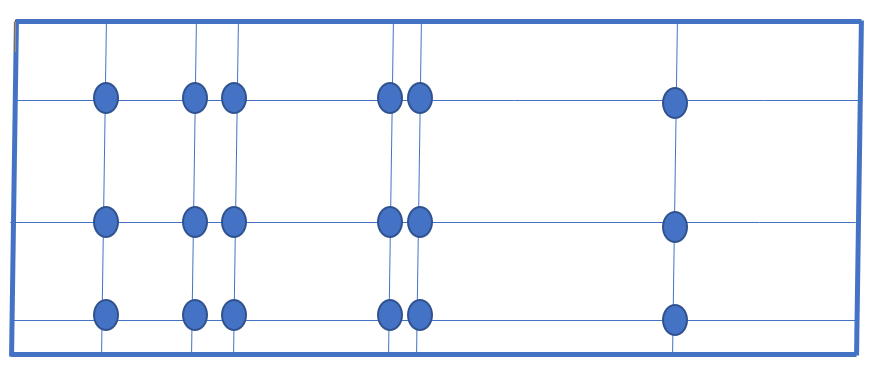
\includegraphics[width=0.4\linewidth]{kronecker}
     \caption{A 2-dimensional rectilinear grid}\label{fig:kronecker}
\end{figure}


In order to use the handy properties of the Kronecker product, we work with a product kernel consisting of the product of the kernels $k_c$  (see equation (\ref{Functional_Product_first_eq})) over scalar inputs. We define $K$ the $n \times n$ gram matrix over $X$ and $K_c$ the $e_c \times e_c$ matrix defined over the vector of scalar inputs $\bm{x}^{(c)}$ and denote with $n = \prod_{c=1}^d e_c$. Imposing the same constraints concerning the indices as in definition (\ref{Kronecker_definition}), we find that  

\begin{equation}\label{Kronecker1}
K(i,j) = K_1(i^{(1)},j^{(1)})K_2(i^{(2)},j^{(2)}) \cdots K_d(i^{(d)},j^{(d)}). 
\end{equation}

In other words, we have that $K = \bigotimes_{c=1}^d K_c$. First let us try to determine the hyperparameters. We again try to optimise the marginal likelihood (\ref{log_marg_llh}). If the spherical noise is zero, the quantity $K^{-1} \bm{y}$ can be found using the Kronecker product. Hence, we only need to compute the inverses of the smaller matrices $K_c$ and execute the corresponding Kronecker product. Calculating the inverses of the smaller matrices has time complexity O($ d \cdot \max\nolimits_{c \in \{1,\cdots,d\}} e_c^3$) and the Kronecker product which is, using the standard matrix-vector multiplication, $O(n^2)$ in runtime and memory. If we calculate the inverses with a Cholesky decomposition, one can again easily compute the determinant of the smaller matrices. Using the corresponding property of determinants of Kronecker products, one can also compute the determinant in a very efficient way. 


However, a small detour has to be made if the spherical noise $\sigma$ is not equal to zero. Despite we can write $K^{-1}$ as a Kronecker product, this is not necessarily the case for $(K + \sigma^2 I)^{-1}$. Luckily, using the eigendecompositions $ K = Q \Lambda Q^t$ of $K$ and  $K_c = Q_c \Lambda_c Q_c^t$ of $K_c$, we find that 

\begin{align}
(K + \sigma I)^{-1} \bm{y} &= Q ( \Lambda + \sigma^2 I)^{-1} Q^t \bm{y} \nonumber \\ 
&= \left( \bigotimes\limits_{c=1}^d Q_c \right)  \left( \left(\bigotimes\limits_{c=1}^d \Lambda_c \right)  + \sigma^2 I \right)^{-1} \left( \bigotimes\limits_{c=1}^d Q^t_c \right) \bm{y}.
\end{align}

Notice that calculating the inverse of is not computationally demanding any more since it is a diagonal matrix. Of course, one needs to calculate the eigenvalues and eigenvectors of the smaller matrices $K_c$ which has time complexity O($ d \cdot \max\nolimits_{c \in \{1,\cdots,d\}} e_c^3$) and the Kronecker product. In \cite{saatcci2012scalable}, one proposes a different approach using tensors for calculating matrix vector products. The necessary basic knowledge of tensors can be found in chapter $26$ of \cite{riley2006mathematical}. This was further clarified in the appendix of \cite{wilson2014covariance}. One found that if the $d$ Kronecker matrices have the same dimension $e = n^{1/d}$, the matrix vector product 
\begin{equation}
K \bm{y} = \bigotimes_{c=1}^d K_c \bm{y}
\end{equation}

can be calculated in $O\left(d \cdot n^{\frac{d+1}{d}} \right)$ in runtime and $O(d n^{\frac{2}{d}})$ in storage. For the determinant we find that 

\begin{align}
| K + \sigma I | = |Q ( \Lambda + \sigma^2 I) Q^t| =  |\Lambda + \sigma^2 I | = \prod_{i=1}^n (\Lambda_{ii} + \sigma^2),
\end{align}

which is not computationally demanding since we already calculated the eigendecomposition. However, note that computational and memory demands scale in dimension, not to mention about the curse of dimensionality. For example, using a dataset with dimension $d =10$ and we only want $3$ different values for each dimension. We have only little information for each dimension although we need $3^{10} = 59049$ data points. Hence, it is not recommended using this technique for datasets with $d > 5$.  Thus, the running time (and feasible accuracy) is very dependent on the dimension, what was not the case before.  


\section{Toeplitz Gaussian Process regression}

Notice that for Kronecker GPR, there is no possible efficiency gain for one dimensional inputs. However, for one dimensional inputs, one can impose a Toeplitz structure on the Gram matrix. This seems not relevant for our subject, since we work with options depending on a lot of variables. Nevertheless, it will be useful in the future. An algorithm about fast inverting a Toeplitz matrix can for example be found in \cite{chan1994circulant}. This algorithm can convert a Toeplitz matrix in $O(n \log{ (n)})$ time.


\chapter{Approximations}

\section{Sparse Gaussian process regression}


In this section, we mainly base us on \cite{quinonero2005unifying} and  \cite{snelson2006sparse} using some statements found in \cite{GPRbook}. The first gives an unifying view of Sparse Gaussian process regression.

In these section we try to find $m < n$ inducing points $\bm{u}$ which are values of the Gaussian process corresponding to a set of input locations $Z$. These points are used to approximate the full covariance matrix over all $n$ training inputs. The determination of the locations of these induction points will be discussed later. An advantage is that we will be able to reduce the running time complexity to $O(nm^2+ m^3)$, and memory requirements $O(mn+m^2)$. 
%Of course, since we reduce the dimension of the covariance matrix, we reduce the number of eigenvectors of the covariance matrix which can be used to fit the data. These methods are called sparse since they are sparse in the data. 

As have been specified in \cite{quinonero2005unifying}, we can see our algorithms as exact inference with an approximated prior. However, In other papers, approximate inference with an exact prior was used. We explain both in order to obtain the necessary intuition. The most basic model we discuss will also be derived using functional analysis. Our Bayesian view in section (\ref{section_bayesian_view}) was very extensive and we really started from scratch; we even did not include kernels. Let us shortly put in order what we have done. We found the predictive distribution by conditioning on the training values $\bm{f}$ and used Bayes. We calculated

\begin{align}\label{integraal}
p(\bm{f}^{\ast}|\bm{y}, \bm{x}^{\ast}, X) &= \int p(\bm{f}^{\ast} | \bm{y}, \bm{f},X, \bm{x}^{\ast}) p(\bm{f} | \bm{y}, X)d\bm{f} \\
 &= \int p(\bm{f}^{\ast} | \bm{y}, \bm{f}, X, \bm{x}^{\ast}) \dfrac{p(\bm{y} |  \bm{f}, X) p(\bm{f}| X )}{ p(\bm{y}| X)} d\bm{f}.
\end{align}


Now, conditioning on the latent variables and assuming $X$ and $\bm{y}$ are independent of $\bm{f}^{\ast}$ given $Z$ and $\bm{u}$, we find that

\begin{align}\label{approximate_llh}
p(\bm{f}^{\ast}|\bm{y}, \bm{x}^{\ast}, X, Z) &= \int p(\bm{f}^{\ast} | \bm{y}, \bm{u},X, \bm{x}^{\ast},Z) p(\bm{u} | \bm{y}, X,Z)d\bm{u} \\
 &= \int p(\bm{f}^{\ast} | \bm{y}, \bm{u},X,\bm{x}^{\ast}, Z) \dfrac{p(\bm{y} | \bm{u}, X,Z) p(\bm{u}| Z )}{ p(\bm{y}| Z,X )} d\bm{u}.
\end{align}

For the view of approximate inference with an exact prior were we replace the likelihood $p(\bm{y} | \bm{u}, X,Z)$ by an approximation  $q(\bm{y} | \bm{u}, X,Z)$. We take $p(\bm{u}|Z) = \mathcal{N}(\bm{0},K_{Z,Z})$ (reasonable since we expect the pseudo data to be distributed as the real data). Calculating this integral gives the predictive distribution. 

Next, we discuss the same using exact inference with an approximated prior. From now on, we also omit the extensive notation including all the covariates for brevity. Using $p(\bm{f}^{\ast} | \bm{f}) p(\bm{f})  = p(\bm{f}^{\ast} , \bm{f})$ we find that 

\begin{equation}
p(\bm{f}^{\ast}|\bm{y})=  \dfrac{1}{ p(\bm{y})}\int  p(\bm{f}^{\ast} , \bm{f}) p(\bm{y} | \bm{f})  d\bm{f}.
\end{equation}
 
As of now, we denote $K(X,X^{\ast}) = K_{X,X^{\ast}}$, which correspond better with the more concise notation. From before, we know that the likelihood $p(\bm{y}|\bm{f}) =  \mathcal{N} (\bm{f}, \sigma^2 I)$ and that 

\begin{equation}
p(\bm{f},\bm{f}^{\ast}) = 
\mathcal{N} \left( \bm{0}, 
\begin{bmatrix}
    K_{X,X} & K_{X,X^{\ast}}\\
    K_{X^{\ast},X}  & K_{X^{\ast},X^{\ast}}
\end{bmatrix} 
\right).
\end{equation}

which we call the GP prior. For brevity, we denote with $Q_{A,B} = K_{A,Z} K_{Z,Z}^{-1} K_{Z,B}$. All the sparse approximations which we are going to discuss can be seen as approximations of the training- and test conditional $p(\bm{f}|\bm{u})$ and $p(\bm{f}^{\ast}|\bm{u})$ given by 

\begin{equation}\label{sparse1}
\begin{aligned}
&p(\bm{f}|\bm{u}) = \mathcal{N}(K_{X,Z} K^{-1}_{Z,Z} \bm{u}, K_{X,X} - Q_{X,X}) \\
&p(\bm{f}^{\ast}|\bm{u}) = \mathcal{N}(K_{X^{\ast},Z} K^{-1}_{Z,Z} \bm{u}, K_{X^{\ast},X^{\ast}} - Q_{X^{\ast},X^{\ast}}). 
\end{aligned}
\end{equation}

Compare this with equation (\ref{function_1_gpr}) and convince yourself that these expression make sense. The matrix $K_{X,Z} K^{-1}_{Z,Z}$ can be seen as some projection matrix absorbing the information of $n$ points in $m$ points. We denote with $q(\bm{f}|\bm{u})$ and $q(\bm{f}^{\ast}|\bm{u})$ their approximations. Approximating the joint prior by assuming that $\bm{f}^{\ast}$ and $\bm{f}$ are conditionally independent given $\bm{u}$, we find that 

\begin{equation}
p(\bm{f}^{\ast},\bm{f}) = \int p( \bm{f}^{\ast},\bm{f} | \bm{u}) p (\bm{u}) d\bm{u}  \simeq  \int q(\bm{f}^{\ast}|\bm{u}) q(\bm{f}|\bm{u}) p(\bm{u}) d\bm{u} = q(\bm{f}^{\ast}, \bm{f}) .
\end{equation}

Notice that due to the assumption of conditional independence, information from $\bm{f}$ can only be transferred to $\bm{f}^{\ast}$ via $\bm{u}$. In our further discussion, we omit the tedious derivations concerning the joint prior/using the approximate likelihood. This will be redundant since in section (\ref{var_regr}), we implicitly do the same calculations.

First, we discuss the Subset of Regressors (SoR) approximation. The name of this method becomes clear in a moment. For this approximation, we use the approximate priors given by 

\begin{equation}
q_{SoR}(\bm{f}|\bm{u}) = \mathcal{N}(K_{X,Z} K^{-1}_{Z,Z} \bm{u} , \bm{0}) \quad \text{and} \quad q_{SoR}(\bm{f}^{\ast} | \bm{u}) =\mathcal{N}(K_{X^{\ast},Z} K^{-1}_{Z,Z} \bm{u} , \bm{0}),
\end{equation}

which are Dirac shaped distributions. The joint prior is given by

\begin{equation}\label{prior_DTC}
q_{SoR}(\bm{f},\bm{f}^{\ast}) = 
\mathcal{N} \left( \bm{0}, 
\begin{bmatrix}
    Q_{X,X} & Q_{X,X^{\ast}}\\
    Q_{X^{\ast},X}  & Q_{X^{\ast},X^{\ast}}
\end{bmatrix} 
\right).
\end{equation}

In this case, the approximate prior is very restrictive. Only a very limited family of functions will be plausible under the posterior, given enough data. This will lead to overconfident predictive variances. However, we are mainly interested in the predictive mean for pricing options so this is not a huge problem. Denoting $\Lambda = \sigma^2 I_n$, the predictive distribution is given by 

\begin{equation}\label{sparse_sor}
q_{SoR} (\bm{f}^{\ast} | \bm{y} ) = \mathcal{N}(Q_{X^{\ast},X}(Q_{X,X} + \Lambda)^{-1}\bm{y}, Q_{X^{\ast} ,X^{\ast}} - Q_{X^{\ast},X}(Q_{X,X} + \Lambda)^{-1} Q_{X,X^{\ast}}).
\end{equation}

This can easily be seen replacing $\bm{f}$ by $\bm{y}$ in equation (\ref{prior_DTC}) and by conditioning the joint distribution on the observations (see appendix section (\ref{Conditioning_of_Gaussians})).  For the next sparse methods, this derivation is always the same and we will not elaborate. 

Notice the strong similarities with equation (\ref{function_1_gpr}). In fact, we have only replaced the matrix $K_{X,X}$ with the matrix $Q_{X,X}$. We actually replace the kernel/covariance function using an approximation, which we discuss in a moment. However, notice that we still have to invert a $n \times n$ matrix. By applying the matrix inversion lemma, we can obtain an expression for the predictive distribution which is more economical to compute. If we denote with $\Sigma = (\Lambda^{-1} K_{Z,X}K_{X,Z} + K_{Z,Z})^{-1}$, the predictive distribution is given by

\begin{equation}\label{pred_SoR}
\boxed{
q_{SoR} (\bm{f}^{\ast} | \bm{y} ) = \mathcal{N}(\Lambda^{-1} K_{X^{\ast},Z} \Sigma K_{Z,X} \bm{y},  K_{X^{\ast},Z} \Sigma K_{Z,X^{\ast}} ).}
\end{equation}

We follow \cite{GPRbook}. Let us try to derive the SoR approximation using functional analysis. We take a subset of regressors (which we also denote with $Z$) and use this to approximate the $i$th eigenfunction. Using equation (\ref{approx_eigenvector}) and denoting with $\lambda_i^{(m)}$ and $u_i^{(m)}$ the eigenvalues and eigenvectors of matrix $K_{Z,Z}$, we find that 

\begin{equation}
\tilde{\varphi}_i (\bm{x}) = \dfrac{\sqrt{m}}{\lambda_i^{(m)}} k_{\bm{x},Z} \bm{u}_i^{(m)}.
\end{equation}

Hence, using $\lambda_i  \approx  \lambda_i^{(m)}/m$, we obtain the following approximation for the kernel $k(\bm{x}, \bm{x}') = \sum\nolimits_{i=1}^n \lambda_i \varphi_i(\bm{x}) \varphi(\bm{x}')$ 

\begin{align}
\tilde{k}_{SoR}(\bm{x}, \bm{x}') &= \sum\limits_{i=1}^m \dfrac{\lambda_i^{(m)}}{m} \tilde{\varphi}_i(\bm{x})\tilde{\varphi}_i(\bm{x}') \nonumber  \\
&= \sum\limits_{i=1}^m  \dfrac{\lambda_i^{(m)}}{m} \dfrac{m}{(\lambda_i^{(m)})^2} k_{\bm{x},Z}  \bm{u}_i^{(m)} (\bm{u}_i^{(m)})^t k_{Z, \bm{x}'} \nonumber \\
&= k_{\bm{x},Z} K_{Z,Z}^{-1} k_{Z, \bm{x}'}.
\end{align}

This is the covariance function used in the SoR. The new covariance function has rank (at most) $m$ (due to the properties of rank and matrix product) and thus this model is a degenerate GP only admitting  $m$ degrees of freedom. Now, equation (\ref{pred_SoR}) can even be derived fulling in the approximations in (\ref{GPR_Bayesian_2}).   


We are ready to discuss the Deterministic Training Conditional (DTC)  approximation. This is an improvement of the SoR approximation  concerning the predictive uncertainties although it has the same predictive mean.  Originally, this method was called Projected Latent Variables (PLV) or Projected Process Approximation (PPA) and seen as a likelihood approximation method where 
\begin{equation}\label{llh_dtc}
p(\bm{y}|\bm{f}) \simeq q(\bm{y}|\bm{u}) = \mathcal{N}(K_{X,Z} K^{-1}_{\bm{u} \bm{u}} \bm{u}, \sigma^2 I_n).
\end{equation}

Notice that we use the projection matrix $K_{X,Z} K^{-1}_{Z,Z}$.  However, looking at it from the view of approximate priors, one imposes a deterministic training conditional (variance $0$) and an exact training conditional (thats why it is called DTC), given by

\begin{equation} \label{dtc}
q_{DTC}(\bm{f}|\bm{u}) = \mathcal{N}(K_{X,Z} K^{-1}_{Z,Z} \bm{u} , \bm{0}), \quad \text{and} \quad q_{DTC}(\bm{f}^{\ast} | \bm{u}) = p (\bm{f}^{\ast}| \bm{u}). 
\end{equation}

The joint prior implied by DTC is given by

\begin{equation}
q_{DTC}(\bm{f},\bm{f}^{\ast}) = 
\mathcal{N} \left( \bm{0}, 
\begin{bmatrix}
    Q_{X,X} & Q_{X,X^{\ast}}\\
    Q_{X^{\ast},X}  & K_{X^{\ast},X^{\ast}}
\end{bmatrix} 
\right).
\end{equation}

Denoting $\Lambda = \sigma^2 I$, one gets that the predictive distribution is given by

\begin{equation}\label{sparse2}
q_{DTC} (\bm{f}^{\ast} | \bm{y} ) = \mathcal{N}(Q_{X^{\ast},X}(Q_{X,X} + \Lambda)^{-1}\bm{y}, K_{X^{\ast} ,X^{\ast}} - Q_{X^{\ast},X}(Q_{X,X} + \Lambda)^{-1} Q_{X,X^{\ast}}).
\end{equation}

Notice the strong similarities with equation (\ref{sparse_sor}) with a small change in the variance. However, we again have to invert a $n \times n$ matrix. By applying the matrix inversion lemma and using the same notation as before, the predictive distribution is given by

\begin{equation}\label{pred_DTC}
\boxed{
q_{DTC} (\bm{f}^{\ast} | \bm{y} ) = \mathcal{N}( K_{X^{\ast},Z} \Sigma K_{Z,X} \Lambda^{-1} \bm{y},   K_{X^{\ast},X^{\ast}} - Q_{X^{\ast},X^{\ast}} + K_{X^{\ast},Z} \Sigma K_{Z,X^{\ast}} ).}
\end{equation}

Hence, we only need to invert a $m \times m$ matrix. It is interesting to notice that the term $K_{X^{\ast},X^{\ast}} - Q_{X^{\ast},X^{\ast}}$ equals $\text{Cov}(\bm{f}^{\ast}|\bm{u})$. This can easily be seen looking at equation (\ref{dtc}). Thus the predictive variance of DTC equals the sum of the predictive variance of the SoR and the predictive variance of $p(\bm{f}^{\ast}|\bm{u})$, which means that the predictive variance of DTC is never smaller than that of SoR . As a remark we also state that the DTC approximation does not exactly corresponds to a Gaussian process since the covariance between latent values depends on whether we work with training or test values as can be seen in equation (\ref{dtc}).
Going in a analogue way, one can also deduce the Fully Independent Training Condition (FITC) approximation. Again, in earlier literature, one called this method Sparse Gaussian Processes using Pseudo-inputs (SGPP) and deduced it from a likelihood approximation 

\begin{equation}
p(\bm{y}|\bm{f}) \simeq q(\bm{y}|\bm{u}) = \mathcal{N}(K_{X,Z} K^{-1}_{U, U} \bm{u}, \text{diag}[K_{X,X}- Q_{X,X}] + \sigma^2 I),
\end{equation}

where one included a diagonal term for the covariance. We can again study it from the view of approximated priors. For the FITC we impose an extra independence assumption for the training  conditional (that's why it is called FITC). We find that, using equation (\ref{sparse1}), 

\begin{equation}
\begin{aligned}
&q_{FITC}(\bm{f}|\bm{u}) = \prod_{i=1}^{n} p(f_i,\bm{u})= \mathcal{N}(K_{X,Z} K^{-1}_{Z,Z} \bm{u} , \text{diag}[K_{X,X} - Q_{X,X}]), \quad \text{and} \quad \\
&q_{FITC}(\bm{f}^{\ast} | \bm{u}) = p(\bm{f}^{\ast}|\bm{u})
\end{aligned}
\end{equation}

The joint prior implied by FITC is given by

\begin{equation}
q_{FITC}(\bm{f},\bm{f}^{\ast}) = 
\mathcal{N} \left( \bm{0}, 
\begin{bmatrix}
    Q_{X,X} - \text{diag}[Q_{X,X} -K_{X,X}] & Q_{X,X^{\ast}}\\
    Q_{X^{\ast},X}  & K_{X^{\ast},X^{\ast}}
\end{bmatrix} 
\right).
\end{equation}

We denote with $\Lambda = \text{diag}[K_{X,X}-Q_{X,X} + \sigma^2 I_n]$. The predictive distribution is given by 

\begin{equation}
q_{FITC} (\bm{f}^{\ast} | \bm{y} ) = \mathcal{N}(Q_{X^{\ast},X}(Q_{X,X} + \Lambda)^{-1}\bm{y}, K_{X^{\ast} ,X^{\ast}} - Q_{X^{\ast},X}(Q_{X,X} + \Lambda)^{-1} Q_{X,X^{\ast}}).
\end{equation}

Notice the strong similarities with equations (\ref{GPR_Bayesian_3}) and (\ref{sparse2}). Rewriting it with $\Sigma = (K_{Z,Z} + K_{Z,X} \Lambda^{-1} K_{X,Z})^{-1}$ and using the matrix inversion lemma, we obtain 

\begin{equation}
\boxed{
q_{FITC} (\bm{f}^{\ast} | \bm{y} ) = \mathcal{N}( K_{X^{\ast},Z} \Sigma K_{Z,X}\Lambda^{-1} \bm{y},   K_{X^{\ast},X^{\ast}} - Q_{X^{\ast},X^{\ast}} + K_{X^{\ast},Z} \Sigma K_{Z,X^{\ast}}) ,}
\end{equation}

which is again more economical to compute. Notice that FITC does not correspond to a GP model since the training and test covariance are not computed the same. If we extend the additional factorizing assumption to the test conditional, one obtains the Fully Independent Conditional (FIC) approximation which is a non-degenerate Gaussian process. The joint prior implied by FIC is given by

\begin{equation}
q_{FIC}(\bm{f},\bm{f}^{\ast}) = 
\mathcal{N} \left( \bm{0}, 
\begin{bmatrix}
    Q_{X,X} - \text{diag}[Q_{X,X} -K_{X,X}] & Q_{X,X^{\ast}}\\
    Q_{X^{\ast},X}  & Q_{X^{\ast},X^{\ast}} - \text{diag}[Q_{X^{\ast},X^{\ast}} -K_{X^{\ast},X^{\ast}}]
\end{bmatrix} 
\right).
\end{equation}

We give a short overview of the approximate kernels we encountered.

\begin{align}\label{sor_and_fic}
& \tilde{k}_{SoR} ({\bm{x}_i,\bm{x}_j}) = k_{\bm{x}_i,Z} K^{-1}_{Z,Z} k_{Z,\bm{x}_j} \\
& \tilde{k}_{FIC} ({\bm{x}_i,\bm{x}_j}) = \tilde{k}_{SoR} ({\bm{x}_i,\bm{x}_j}) + \delta_{i,j} \left( k ({\bm{x}_i,\bm{x}_j}) - \tilde{k}_{SoR} ({\bm{x}_i,\bm{x}_j}) \right).
\end{align}

\iffalse

\begin{equation}
\begin{aligned}
&q_{FITC}(\bm{f}|\bm{u}) = \prod_{i=1}^{n} p(f_i,\bm{u})= \mathcal{N}(K_{X,Z} K^{-1}_{Z,Z} \bm{u} , \text{diag}[K_{X,X} - Q_{X,X}]), \quad \text{and} \quad \\
&q_{FITC}(\bm{f}^{\ast} | \bm{u}) = \prod_{i=1}^{n} p(f_i^{\ast},\bm{u}) = \mathcal{N}(K_{X^{\ast},Z} K^{-1}_{Z,Z} \bm{u} , \text{diag}[K_{X^{\ast},X^{\ast}} - Q_{X^{\ast},X^{\ast}}])
\end{aligned}
\end{equation}

The joint prior implied by FIC is given by

\begin{equation}
q_{FITC}(\bm{f},\bm{f}^{\ast}) = 
\mathcal{N} \left( \bm{0}, 
\begin{bmatrix}
    Q_{X,X} - \text{diag}[Q_{X,X} -K_{X,X}] & Q_{X,X^{\ast}}\\
    Q_{X^{\ast},X}  & Q_{X^{\ast},X^{\ast}} - \text{diag}[Q_{X^{\ast},X^{\ast}} -K_{X^{\ast},X^{\ast}}]
\end{bmatrix} 
\right).
\end{equation}
\fi

Now we are ready to discuss how to select the inducing variables. We discuss three methods although there are much more different approaches possible. One can just use a subset of the data. However, this is often not sufficient so one can use K-means (see appendix section (\ref{appendix_kmeans})) such that each latent variable represents a cluster of the data. The time complexity of LLoyd's algorithm with $p$ iterations is $O(nmdp)$. For large datasets, it is recommended to use mini-batching.  Another approach is maximising the marginal likelihood (evidence) with respect to $Z$ like in \cite{snelson2006sparse}. For the different models, using the right $\Lambda$, the evidence is given by 

\begin{equation}\label{log_marg_ind_input}
\log ( q(\bm{y}|Z)) = -\dfrac{1}{2} \text{log}|Q_{X,X}+\Lambda| - \dfrac{1}{2} \bm{y}^t (Q_{X,X} + \Lambda)^{-1} \bm{y} - \dfrac{n}{2} \log{(2\pi)}.
\end{equation}


\begin{Theorem}[Computation and storage costs evidence sparse methods]\label{time_compl_evid_approx}
The computational cost of equation (\ref{log_marg_ind_input}) is $O(nm^2 + m^3)$ and the storage demands equals $O(nm + m^3)$.
\end{Theorem}

\begin{proof}
The matrix inversion lemma does the major part of the work. As one can suspect, the first term comes from a matrix matrix multiplication with dimensions $m \times m$ and $m \times n$ and the second a matrix inversion of dimension $m \times m$.  Let us give the derivation. We find by  writing $K_{Z,Z} = L_{Z}  L_{Z}^t$ that 

\begin{equation}
\begin{aligned}
(Q_{X,X} + \Lambda) ^{-1} &= (K_{X,Z} K_{Z,Z}^{-1} K_{Z,X} + \Lambda)^{-1}  \\
&= (K_{X,Z}  (L_{Z}^t)^{-1} I_m (L_{Z})^{-1} K_{Z,X} + \Lambda)^{-1}  \\
&= \Lambda^{-1} - \Lambda^{-1} K_{X,Z} \\ 
& \quad (L_{Z}^t)^{-1} ( I_m + L_{Z}^{-1} K_{Z,X} \Lambda^{-1} K_{X,Z} (L_{Z}^t)^{-1} )^{-1} L_{Z}^{-1} K_{Z,X} \Lambda^{-1}.
\end{aligned}
\end{equation}

Now, the we need to take the inverse of a $m \times m$ matrix which took $O(nm^2)$ time to evaluate. Using Cholesky, we find that 

\begin{equation}\label{Sparse_efficient_cal}
( I_m + L_{Z}^{-1} K_{Z,X} \Lambda^{-1} K_{X,Z} (L_{Z}^t)^{-1} ) = \mathcal{L}_{Z,Z} \mathcal{L}_{Z,Z}^t
\end{equation}

and thus we can write 

\begin{equation}
(Q_{X,X} + \Lambda) ^{-1} =  \Lambda^{-1} - \Lambda^{-1} K_{X,Z}(L_{Z}^t)^{-1} (\mathcal{L}_{Z,Z}^t)^{-1} (\mathcal{L}_{Z,Z})^{-1}  L_{Z}^{-1} K_{Z,X} \Lambda^{-1}.
\end{equation}

Hence, we only need to invert a diagonal matrix of dimension $n \times n$ and two matrices of dimension $m \times m$. Multiplying this expression with $\bm{y}$ results in a time complexity of $O(nm)$. Using Sylvester’s Determinant Theorem (see appendix section (\ref{Sylvester})), one can see that the determinant can be calculated in a very economical way. We find that

\begin{equation}
\begin{aligned}
\det{(Q_{X,X} + \Lambda)} &= \det{(\Lambda)} \det({\Lambda^{-1} Q_{X,X} + I_n)} \\
&=  \det{(\Lambda)} \det{(\Lambda^{-1} K_{X,Z}} (L_{Z} ^t)^{-1} L_{Z}^{-1}  K_{Z,X} + I_{n}) \\
&= \det{(\Lambda)}  \det{( I_{m} + (L_{Z}) ^{-1} K_{Z,X} \Lambda^{-1} K_{X,Z} (L_{Z}^t)^{-1} ) }
\end{aligned}
\end{equation}

Notice that the first determinant is just the product of the diagonal elements of $\Lambda$ and that the second term equals equation (\ref{Sparse_efficient_cal}). Since, we already calculated the Cholesky decomposition, we just need to calculate the product of squares of the diagonal elements. However, we need to calculate the logarithm of this determinant, thus we just need to calculate the sum of the logarithms of these diagonal elements. As a remark, in order to calculate $\Lambda$, one only needs the diagonal elements of $K_{X,X}$ (and if necessary $Q_{X,X}$).

Since one has to construct the matrix $K_{Z,X}$, its transpose and some $m \times m$ matrices, the storage demands are $O(nm +m^2)$.
\end{proof}

\begin{Theorem}[Computation cost prediction sparse methods]
The computational cost to find the predictive mean for one observation using sparse methods is $O(m)$.
\end{Theorem}

\begin{proof}
The vector $\Sigma K_{Z,X}\Lambda^{-1} \bm{y}$ has been calculated during training. Hence, the construction and vector multiplication with $k_{\bm{x}^{\ast},Z}$ only takes $O(m)$ time. 
\end{proof}

Notice that we now have to fit $md$ + $\Theta$ parameters and overfitting can occur. In other words, the locations $Z$ form a set of extra hyperparameters. Furthermore, optimising more variables requires more time. Hence, using K-means is recommended. However, we find a more rigorous solution solving overfitting in the next section. 


\section{Variational Gaussian Process Regression}\label{var_regr}

However, one can also optimise inducing point locations as part of the model like in \cite{titsias2009variational} and \cite{hensman2013gaussian}. The inducing points positions are variational parameters rather than model parameters and are thus protected from overfitting. Readers which are not familiar with Variational learning are referred to section (\ref{KL}) in the appendix.

Like before, we consider the following 

\begin{equation}\label{variational_start}
\begin{aligned}
&p(\bm{y}|\bm{f}) = \mathcal{N}(\bm{y} | \bm{f}, \sigma^2 I_n) \\
&p(\bm{f}|\bm{u}) = \mathcal{N} (\bm{f}|K_{X,Z} K^{-1}_{Z,Z} \bm{u} , K_{X,X} - Q_{X,X}) \\
&p(\bm{u}) = \mathcal{N}( \bm{u} | \bm{0}, K_{Z,Z})
\end{aligned}
\end{equation}

First, we try to obtain a lower bound of $p(\bm{y}|\bm{u})$, which is also know as the variational or evidence lower bound (ELBO), but now given the inducing points. Using Bayes on ${p(\bm{f}|\bm{y},\bm{u})}$ and after an algebraic manipulation, we find that

\begin{align}
p(\bm{y}|\bm{u}) = \dfrac{p(\bm{y}|\bm{f}, \bm{u})p(\bm{f}|\bm{u})}{p(\bm{f}|\bm{y},\bm{u})}.
\end{align}

Taking the natural logarithm, we obtain that

\begin{equation}
\log{(p(\bm{y}|\bm{u})}) = \log{(p(\bm{y}|\bm{f}, \bm{u})}) + \log{\left(\dfrac{p(\bm{f}|\bm{u})}{p(\bm{f}|\bm{y},\bm{u})}\right)}
\end{equation}

Since the left hand side is not a function of $\bm{f}$, we find by taking the expectation to $p(\bm{f}|\bm{u})$ that 

\begin{equation}\label{sparse_var_1}
\log{(p(\bm{y}|\bm{u})}) = \mathbb{E}_{p(\bm{f}|\bm{u})}\log{(p(\bm{y}|\bm{f}, \bm{u})}) + \mathbb{E}_{p(\bm{f}|\bm{u})} \left[ \log{\left(\dfrac{p(\bm{f}|\bm{u})}{p(\bm{f}|\bm{y},\bm{u})}\right)} \right]
\end{equation}

Note that the last term is the Kullback Leibler (KL) divergence between the posterior of $\bm{f}$ given the data and the
inducing variables and the posterior of $\bm{f}$ given the inducing variables only. From now, we denote that $ \tilde{p}(\bm{y}|\bm{u}) = \mathbb{E}_{p(\bm{f}|\bm{u})}\log{(p(\bm{y}|\bm{f}, \bm{u})})$ (it is independent of $\bm{f}$). Hence we can write that 

\begin{equation}\label{sparse_var_5}
\log{(p(\bm{y}|\bm{u})}) = \tilde{p}(\bm{y}|\bm{u}) + \text{KL}[p(\bm{f}|\bm{u})|p(\bm{f}||\bm{y},\bm{u})].
\end{equation}

Since $p(\bm{y}|\bm{f})$ is separable across the data

\begin{equation}
p(\bm{y}|\bm{f}) = \prod_{i=1}^{n} p(y_i|f_i),
\end{equation}


the following lemma can be found

\begin{Lemma}[Expression of $\bm{\exp (\tilde{p}(\bm{y}|\bm{u}) )}$]\label{lemma_bound1}
The following equation can be found 
\begin{align}\label{sparse_var_2}
\exp (\tilde{p}(\bm{y}|\bm{u}) )&= \mathcal{N} (\bm{y}|K_{X,Z} K^{-1}_{Z,Z} \bm{u}, \sigma^2 I_n ) \exp{ \left( -\dfrac{1}{2\sigma^2} \Tr ( K_{X,X} - Q_{X,X} ) \right)} \nonumber \\
&= \prod_{i=1}^n \mathcal{N}(y_i|k_{\bm{x}_i,\bm{z}} K^{-1}_{Z,Z} \bm{u} , \sigma^2) \exp{\left(-\dfrac{1}{2\sigma^2}(k_{\bm{x}_i,\bm{x}_i} - k_{\bm{x}_i,\bm{z}} K^{-1}_{Z,Z}k_{\bm{z},\bm{x}_i}) \right)} .
\end{align}
\end{Lemma}

\begin{proof}
We find that
\begin{align}
\tilde{p}(\bm{y}|\bm{u}) &=  \mathbb{E}_{p(\bm{f}|\bm{u})}\log{(p(\bm{y}|\bm{f})}) \nonumber \\
&= \int p(\bm{f}|\bm{u}) \log (p(\bm{y}|\bm{f})d \bm{f} \nonumber \\
&= \int p(\bm{f}|\bm{u}) \left( -\dfrac{n}{2} \log(2 \pi \sigma^2) - \dfrac{1}{2 \sigma^2} \Tr \left( ( \bm{y} - \bm{f})^2  \right) \right) d\bm{f} \nonumber \\
&=  - \dfrac{n}{2} \log (2 \pi \sigma^2) \int p(\bm{f} | \bm{u}) d\bm{f} - \dfrac{1}{2 \sigma^2} \int p(\bm{f} | \bm{u}) \Tr \left( \bm{y} \bm{y}^t - 2 \bm{y}\bm{f}^t - \bm{f}\bm{f}^t   \right) d\bm{f}
\end{align}

Now, we denote with $\bm{\alpha} = \mathbb{E}(\bm{f}|\bm{u})$. Noting that the variance equals the difference between the second moment and the first moments squared, we find that 

\begin{align}\label{equation_VFE}
\tilde{p}(\bm{y}|\bm{u}) &=  - \dfrac{n}{2} \log (2 \pi \sigma^2) - \dfrac{1}{2 \sigma^2} \Tr \left( \bm{y} \bm{y}^t - 2 \bm{y}\bm{\alpha}^t - \bm{\alpha}\bm{\alpha}^t + K_{X,X} - Q_{X,X}  \right) \nonumber \\ &= \log{ \mathcal{N}(\bm{y} | \bm{\alpha}, \sigma^2 I} ) - \dfrac{1}{2\sigma^2} \Tr (K_{X,X} - Q_{X,X}).
\end{align}
We can find the solution by taking the exponential. 
\end{proof}


Hence, equation (\ref{equation_VFE}) is a lower bound of $p(\bm{y}|\bm{u})$ which is separable across $\bm{y}$ and consists of a likelihood approximation and a penalty term. Our goal is to minimize the KL divergence, which is the goal of variational inference. Hence, instead of modifying the exact GP model, we minimize the distance between the exact posterior GP and a variational approximation. In other words, we want that $p(\bm{f}|\bm{u})$ is similar to $p(\bm{f}|\bm{y}, \bm{u})$.Let us first discuss the case were the inducing variables are placed at the training data locations ($X = Z$). The penalty term in equation (\ref{equation_VFE}) equals one and the KL divergence equals zero. When $m<n$ we can minimize the KL with respect to $Z$. This insures that $Z$ is distributed amongst the training data $X$ such that the penalty term is small. Using this, we can find a variational lower bound for the true log marginal likelihood $\log{(p(\bm{y}|X))} $ (evidence) which was derived by \cite{titsias2009variational}. 

\begin{Theorem}
A variational lower bound for the evidence is given by

\begin{align}\label{sparse_var_3}
\log(p(\bm{y}|X)) &= \log( \int p(\bm{y}|\bm{u})p(\bm{u})d\bm{u} \geq \log(\int \exp(\tilde{p}(\bm{y}|\bm{u})) p(\bm{u}) d\bm{u} \nonumber \\
&= \log \mathcal{N} (\bm{y}|\bm{0},\sigma^2 I_n + Q_{X,X}) - \dfrac{1}{2 \sigma^2} \Tr (K_{X,X} - Q_{X,X}).
\end{align}

\end{Theorem}

\begin{proof}
The inequality follows from equation (\ref{sparse_var_5}) and the fact that $KL(\cdot) \geq 0$. Using lemma (\ref{lemma_bound1}) in the appendix section (\ref{Conditioning_of_Gaussians}), we find that 
\begin{align}
 & \quad \log(\int \exp(\tilde{p}(\bm{y}|\bm{u})) p(\bm{u}) d\bm{u}) \nonumber \\ &= \log \left( \int  \mathcal{N}(\bm{y} | \bm{\alpha}, \sigma^2 I ) \mathcal{N}(\bm{u} | \bm{0}, K_{Z,Z} ) d \bm{u} \right)  - \dfrac{1}{2 \sigma^2} \Tr ( K_{X,X} - Q_{X,X}) \nonumber \\   &= \log  \left( \int  \mathcal{N}(\bm{y} | \bm{\alpha}, \sigma^2 I ) \mathcal{N}(\bm{\alpha} | \bm{0}, Q_{X,X} ) d \bm{\alpha} \right)  - \dfrac{1}{2 \sigma^2} \Tr ( K_{X,X} - Q_{X,X}) \nonumber \\ &= \log {(N(\bm{y}|\bm{0}, \sigma^2 I + Q_{X,X}))- \dfrac{1}{2 \sigma^2} \Tr (K_{X,X} - Q_{X,X})}.
\end{align}
\end{proof}

Notice that the first term is the same as equation (\ref{log_marg_ind_input}). However, the variational method is completely different as the other inducing point methods concerning the selection of the inducing inputs and the kernel hyperparameters due to the extra regularisation term in equation (\ref{sparse_var_3}). As has been said before, the inducing point locations $Z$ can be seen as variational parameters instead of an extra set of hyperparameters. The method optimising equation \ref{sparse_var_3} is called the VFE (Variational Free Energy) method.

The matrix $(K_{X,X} - Q_{X,X})$ equals $\text{Cov}(\bm{f}|\bm{u})$, which corresponds to the squared error of prediction the training values $\bm{f}$ from the inducing variables $\bm{u}$ which equals zero if $X=Z$. Titsias stated that this trace term protect against overfitting takes care of selecting good inducing points. The lower bound (\ref{sparse_var_3}) has again a computational complexity of $O(nm^2 + m^3)$ and storage demands of $O(nm + m^3)$. In order to compute the trace, one only needs the diagonal elements of $K_{X,X}$ and we do not need to calculate the whole kernel. 

Next, using $p(\bm{u})$ and the approximation $\exp{( \tilde{p}(\bm{y}|\bm{u})})$ for $p(\bm{y}|\bm{u})$, we find that

\begin{align}\label{marg_on_u}
q(\bm{u}|\bm{y}) &\propto \exp{ \tilde{p}(\bm{y}|\bm{u})) p(\bm{u})  }\nonumber \\
&\propto \mathcal{N}(\bm{y} | \bm{\alpha}, \sigma^2 I_n)  p(\bm{u}) \nonumber \\
&= c \exp{ \left( \dfrac{1}{2\sigma^2} \bm{u}^t K_{Z,Z}^{-1} K_{Z,X} K_{X,Z} K_{Z,Z}^{-1} \bm{u} + \dfrac{1}{\sigma^2} \bm{y}^t K_{X,Z} K_{Z,Z}^{-1} \bm{u} + \dfrac{1}{2\sigma^2} \bm{u} K_{Z,Z}^{-1} \bm{u} \right) },
\end{align}

where $c$ is a constant. By completing the square and denoting with $\Sigma = (\Lambda^{-1} K_{Z,X}K_{X,Z} + K_{Z,Z})^{-1}$, we recognise a Gaussian and find that

\begin{equation}\label{optimal_q}
q(\bm{u}|\bm{y}) =  \mathcal{N} (\bm{u}|\sigma^{-2} K_{Z,Z} \Sigma K_{Z,X} \bm{y}, K_{Z,Z}\Sigma K_{Z,Z}^{-1}).
\end{equation}

Now, using equation (\ref{approximate_llh}), we find that 

\begin{align} \label{mean_predicitive_dtc}
\mathbb{E} [q(\bm{f}^{\ast}|\bm{y})] &= \int \mathbb{E} [p(\bm{f}^{\ast}|\bm{u})] q(\bm{u}|\bm{y}) d\bm{u}  \nonumber \\
&= \int K_{X^{\ast},Z} K_{Z,Z}^{-1} \bm{u} q(\bm{u}|\bm{y}) d\bm{u} \nonumber \\
&= K_{X^{\ast},Z} K_{Z,Z}^{-1} \mathbb{E} [q(\bm{u}|\bm{y})] \nonumber \\ &= \sigma^{-2} K_{X^{\ast},Z} \Sigma K_{Z,X} \bm{y},
\end{align}

which is the same as for DTC. This makes sense since $\exp{ \tilde{p}(y|u))}$ is equal to equation (\ref{llh_dtc}). In the previous section, we mainly focussed on deriving the predictive distribution with approximate priors, although this can also be done using likelihood approximations as has been shown here. A logical extension will be a variational extension for the FITC. For the DTC we have that $\Lambda = \sigma^2 I$ and for FITC we have that $\Lambda = \text{diag}[K_{X,X}-Q_{X,X} + \sigma^2 I]$. Hence replacing $\sigma^2 I$ in equation (\ref{variational_start}) by $\Lambda$, we find a generalisation which may be suitable if one wants to include input-dependent variance.


We omit the derivation for the predictive variance since we are mainly interested for the predictions and the calculations are tedious. Despite the approach is different in both \cite{titsias2009variational} and \cite{GPRbook} (chapter $8$), some concise derivations can be found. One finds that 

\begin{equation}
\mathbb{V} [q(\bm{f}^{\ast}|\bm{y})] =  K_{X^{\ast},X^{\ast}} - Q_{X^{\ast},X^{\ast}} + K_{X^{\ast},Z} \Sigma K_{X^{\ast},Z}^t,
\end{equation}

with $\Sigma$ defined as before. 

A thorough discussion concerning the difference in behaviour of the FITC and the standard VFE approximation can be found in \cite{bauer2016understanding} which is definitely worth a read. We give a short resume of this paper since the behaviour of the FITC and VFE can be explained thanks to these results which comes at handy in the data study. Suppose we also train the noise variance parameter $\sigma$. We have that the evidence/lower bound for FITC and VFE is given by

\begin{equation}\label{log_marg_ind_input}
\text{Objective} = \underbrace{-\dfrac{1}{2} \text{log}|Q_{X,X}+\Lambda|}_{\text{Complexity penalty}} - \underbrace{\dfrac{1}{2} \bm{y}^t (Q_{X,X} + \Lambda)^{-1} \bm{y}}_{\text{Data Fit}} - \underbrace{\dfrac{1}{2 \sigma^2} \Tr (T)}_{\text{Trace Term}} - \dfrac{n}{2} \log{(2\pi)} .
\end{equation}
were the interpretation of the parameters may be different for each method. The trace term $T$ equals $0$ for the FITC for example.

First, FITC can severely underestimate the noise variance and VFE tends to overestimate it. The diagonal term $\text{diag}( K_{X,X} - Q_{X,X})$ is zero close to an inducing point and grows to the prior variance away from an inducing point. It can be seen as a heteroscedastic noise term. For data points far from the mean and the inducing points, the data fit term is small since the heteroscedastic noise term has increased. Hence, $\sigma^2$ looses his meaning and can decreased to reduce the complexity penalty. In extreme cases, $\sigma^2$ can be estimated to be almost zero. Next, VFE tends to over-estimate the noise variance because both the data fit and trace term can be reduced by increasing $\sigma^2$.

Furthermore, VFE always improves by including additional inducing inputs although FITC may ignore them. Adding an inducing point can be seen as a rank $1$ update of $Q_{X,X}$ and is always advantageous for the VFE bound. For FITC, the heteroscedastic noise term decreases at all points which reduces the complexity penalty but worsens the data fit penalty.

By placing the inducing points on every training input, VFE and FITC both recover the true posterior. This equals the global optimum for VFE since the KL gap to the true marginal likelihood is zero.  Notice that the lower bound (\ref{sparse_var_3}) just becomes the evidence. However, the objective function of FITC can still be improved with clumping of inducing points. 

Finally, they stated that the objective function of VFE is harder to optimise than FITC due to more amenable local optima. 

Although this is maybe the best that we have found so far we can still obtain a faster algorithm. 
%Although this is maybe the best that we have found so far, we still have the annoying `n' for computational and storage.  Now, brace yourself for the culmination of Gaussian Process regression, where the computational complexity equals $O(m^3)$!

\section{Stochastic Variational Gaussian Process Regression}

\begin{figure}[!htb]
   \begin{minipage}{0.31\textwidth}
     \centering
     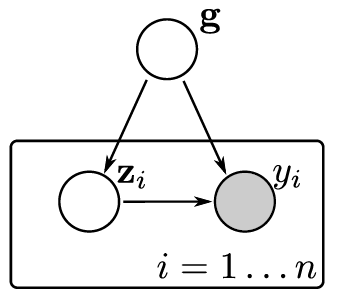
\includegraphics[width=1.1\linewidth]{plot_variational_inference}
     \caption{Requirements for SVI}\label{fig:var_1.1}
   \end{minipage}\hfill
   \begin{minipage}{0.31\textwidth}
     \centering
     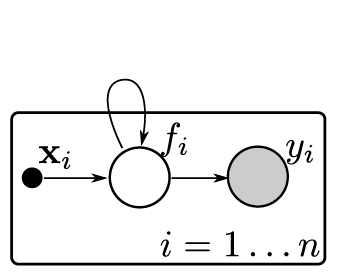
\includegraphics[width=1.1\linewidth]{plot_GPR_regression}
     \caption{Standard GPR}\label{fig:var_1.2}
   \end{minipage}\hfill
   \begin {minipage}{0.31\textwidth}
     \centering
     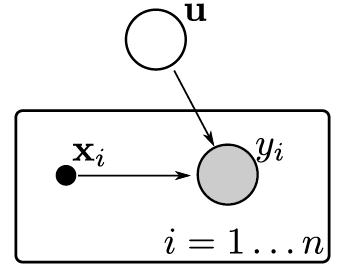
\includegraphics[width=1.1\linewidth]{plot_variational_regression}
     \caption{Variational GPR}\label{fig:var_1.3}
   \end{minipage}
   \caption*{All plots are from \cite{hensman2013gaussian}}
\end{figure}


More information and assumptions of stochastic variational inference can be found in the appendix section (\ref{appendix_var_inf}). As have been stated in \cite{hensman2013gaussian} and in the appendix, we must have a set of global variables and $\bm{y}$ factorises in the latent variables (figure \ref{fig:var_1.1}). In figure \ref{fig:var_1.2}), one can see a plot of standard GPR were the connectivity between the values of $\bm{f}$ is denoted by a loop. In stochastic variational GPR, the variables $\bm{u}$ fulfil the role of global variables (figure \ref{fig:var_1.3}), which will enable stochastic variational inference. We use the term $\tilde{p}(\bm{y}|\bm{u})$ which act as $\log(p(y_i | \bm{u}, \bm{x}_i)$.  One finds the DTC formulation by marginalising on $\bm{u}$ which introduces dependencies between the observations (see equation (\ref{marg_on_u}) and (\ref{mean_predicitive_dtc})).

We introduce a variational distribution $q(\bm{u}) = \mathcal{N}(\bm{u}|\bm{m},S)$. Now we can find another lower bound $\mathcal{L}_1$ of $p(\bm{y}|X)$ (the evidence). By writing $p(\bm{u},\bm{y}) = p(\bm{u}|\bm{y}) p(\bm{y})$, we find that 

\begin{equation}
\text{KL}[q(\bm{u})||p(\bm{u}|\bm{y})] = \mathbb{E}_{q(\bm{u})}[\log{q(\bm{u}}))] - \mathbb{E}_{q(\bm{u})}[\log(p(\bm{u},\bm{y}))] + \log(p(\bm{y}|X)).
\end{equation}

Then defining $\mathcal{L}_1$ as  

\begin{equation}
\mathcal{L}_1 =  -\mathbb{E}_{q(\bm{u})}[\log({q(\bm{u}}))] + \mathbb{E}_{q(\bm{u})}[(\log(p(\bm{u},\bm{y}))],
\end{equation}

we find that

\begin{equation}
\log{(p(\bm{y}|X)}) = \text{KL}[q(\bm{u})||p(\bm{u}|\bm{y})] + \mathcal{L}_1. 
\end{equation}

Since that $KL(\cdot) \geq 0$, we find that $\mathcal{L}_1$ is indeed a lower bound for the evidence. Hence, maximising this bound makes the KL-divergence between $p(\bm{u}|\bm{y})$ and $q(\bm{u})$ minimal. In other words, $q(\bm{u})$ will be similar to the true posterior $p(\bm{u}|\bm{y})$. Next, we use $p(\bm{u},\bm{y}) = p(\bm{\bm{y}|\bm{u}})p(\bm{u})$ and find that

\begin{align}
\mathcal{L}_1 &= -\mathbb{E}_{q(\bm{u})}[\log({p(\bm{u}}))] + \mathbb{E}_{q(\bm{u})}[(\log(p(\bm{y}|\bm{u}))]+ \mathbb{E}_{q(\bm{u})}[\log({q(\bm{u}}))] \nonumber \\
&= \mathbb{E}_{q(\bm{u})}[(\log(p(\bm{y}|\bm{u}))] - \text{KL}[q(\bm{u})||p(\bm{u})] 
\end{align}

From equation (\ref{sparse_var_5}), we thus see that $\mathcal{L}_1$ is dependent on $\bm{f}$. In order to execute stochastic variational inference, this may not be the case. Hence, we calculate the lower bound given by

\begin{align}
\mathcal{L}_1 \geq \mathbb{E}_{q(\bm{u})}[\tilde{p}(\bm{y}|\bm{u})] - \text{KL}[q(\bm{u})||p(\bm{u})]
\end{align}


Finally we find a lower bound independent of $\bm{f}$ for the evidence given by 

\begin{equation}\label{l2bound}
\log{(p(\bm{y}|X)}) \geq \mathcal{L}_1 \geq \mathbb{E}_{q(\bm{u})}[\tilde{p}(\bm{y}|\bm{u})] - \text{KL}[q(\bm{u})||p(\bm{u})] = \mathcal{L}_2,
\end{equation}

which we will try to maximise. The previous derivation of the lower bound $\mathcal{L}_2$ was derived focussing on the independence of $\bm{f}$. Now, we derive it using a more intuitive approach. In variational inference, we always want to minimise the KL-divergence between approximate variational posterior $q$ and the true posterior $p$. Notice that $\bm{f}$ and $\bm{u}$ are the free parameters of the model. Now, choosing a variational posterior 

\begin{equation}
q(\bm{f}, \bm{u}) = p(\bm{f}|\bm{u}) = p(\bm{f}| \bm{u}) q(\bm{u}),
\end{equation}

and noticing that $KL(\cdot) \geq 0$, we find that 

\begin{equation}\label{variational}
\begin{aligned}
0 & \geq - \text{KL}[q(\bm{f}, \bm{u}) || p(\bm{f}, \bm{u} |\bm{y})]  \\ &= \mathbb{E}_{q(\bm{f}, \bm{u})} \log \left( \dfrac{p(\bm{f}, \bm{u}| \bm{y})}{q(\bm{f}, \bm{u}) }\right) \\
&= \mathbb{E}_{q(\bm{f},\bm{u})} \log \left( \dfrac{p(\bm{y}|\bm{f}, \bm{u})p(\bm{f}|\bm{u})p(\bm{u})}{p(\bm{y})p(\bm{f}|\bm{u}) q(\bm{u})} \right) \\
&= \int \int \log \left( \dfrac{p(\bm{y}|\bm{f}, \bm{u}) p(\bm{u})}{p(\bm{y}) q(\bm{u})}\right)  q(\bm{f}, \bm{u}) d\bm{f} d\bm{u}  \\
&= \int \int \log \left( \dfrac{p(\bm{u})}{q(\bm{u})} \right) q(\bm{u}, \bm{f}) d\bm{f} d\bm{u} + \int \int \log  \left( \dfrac{p(\bm{y}| \bm{f} , \bm{u})}{p(\bm{y})} \right) q(\bm{f}, \bm{u}) d\bm{f} d\bm{u} \\ 
&= \int \int \log \left( \dfrac{p(\bm{u})}{q(\bm{u})} \right) q(\bm{u}) d\bm{u} + \int \int \log(p(\bm{y}| \bm{f} , \bm{u})) p(\bm{f}|\bm{u}) q(\bm{u})  d\bm{f} d\bm{u} - \log (p(\bm{y})) \\
&= - \text{KL}[q(\bm{u})||p(\bm{u})] + \mathbb{E}_{q(\bm{u})}[\mathbb{E}_{p(\bm{f}| \bm{u})} \log (p(\bm{y}| \bm{f}, \bm{u})] - \log (p(\bm{y}))  \\
&= - \text{KL}[q(\bm{u})||p(\bm{u})] + \mathbb{E}_{q(\bm{u})}[\tilde{p}(\bm{y}|\bm{u})] - \log (p(\bm{y})).
\end{aligned}
\end{equation}

Hence we find that 

\begin{equation}
\log (p(\bm{y})) \geq - \text{KL}[q(\bm{u})||p(\bm{u})] + \mathbb{E}_{q(\bm{u})}[\tilde{p}(\bm{y}|\bm{u})] = \mathcal{L}_2.
\end{equation}







As denoted before, we have that $q(\bm{u}) = \mathcal{N}(\bm{u}|\bm{m},S)$. The following lemma can be found. 

\begin{Lemma}

Denoting with $\Gamma_i = \frac{1}{\sigma^2}K_{Z,Z}^{-1} k_{Z,\bm{x}_i} k_{\bm{x}_i,Z} K_{Z,Z}^{-1}$, $\mathcal{L}_2$ has the following explicit expression

\begin{align}\label{Stochastvargpr}
\mathcal{L}_2 = \sum\limits_{i=1}^{n} \left\{ \log{\mathcal{N}(y_i|k_{\bm{x}_i,Z} K_{Z,Z}^{-1} \bm{m}, \sigma^2}) - \dfrac{1}{2 \sigma^2} (k_{\bm{x}_i,\bm{x}_i} - q_{\bm{x}_i,\bm{x}_i}) - \dfrac{1}{2}\Tr(S\Gamma_i)  \right\} \nonumber \\
- \text{KL}[q(\bm{u})||p(\bm{u})]
\end{align}

\end{Lemma}



\begin{proof}
The origin of the Kullback-Leiber component in equation (\ref{Stochastvargpr}) is obvious. We find that
\begin{align}
\mathbb{E}_{q(\bm{u})}[\tilde{p}(\bm{y}|\bm{u})]
&= \int q(\bm{u}) \tilde{p}(\bm{y}|\bm{u}) d\bm{u} \nonumber \\
&= \int q(\bm{u}) \left( \log \left( \mathcal{N}(\bm{y}|\bm{\alpha},\sigma^2 I_n) \right) - \dfrac{1}{2 \sigma^2} \Tr (K_{X,X} - Q_{X,X}) \right) d\bm{u} \nonumber \\
&= \int q(\bm{u}) \left( \log \left( \mathcal{N}(\bm{y}|\bm{\alpha},\sigma^2 I_n) \right) \right) d\bm{u} - \sum\limits_{i=1}^{n} \dfrac{1}{2 \sigma^2} (k_{\bm{x}_i,\bm{x}_i} - q_{\bm{x}_i,\bm{x}_i}),
\end{align} 
since the integral of a density function equals one. Hence, the trace term is equal to the middle term in equation (\ref{Stochastvargpr}). By omitting this term we find
\begin{align}
\int q(\bm{u}) \log \left( \mathcal{N}(\bm{y}|\bm{\alpha},\sigma^2 I_n) \right) d\bm{u}
&= \int q(\bm{u}) \left( -\dfrac{n}{2} \log(2 \pi \sigma^2) - \dfrac{1}{2 \sigma^2} \Tr \left( ( \bm{y} - \bm{\alpha})^2  \right) \right) d\bm{u} \nonumber \\
&=  - \dfrac{n}{2} \log (2 \pi \sigma^2) - \dfrac{1}{2 \sigma^2} \int q(\bm{u}) \Tr \left( \bm{y} \bm{y}^t - 2 \bm{y}\bm{\alpha}^t - \bm{\alpha}\bm{\alpha}^t   \right) d\bm{u}.
\end{align}

Now, remember that $q(\bm{u}) = \mathcal{N}(\bm{u}|\bm{m},S)$ and  we denote with $\bm{\beta} = K_{X,Z} K_{Z,Z}^{-1} \bm{m}$. Noting that the variance equals the difference between the second moment and the first moment squared and that matrices in a trace of a product can be switched, we find that 

\begin{align}
\mathbb{E}_{q(\bm{u})}[\tilde{p}(\bm{y}|\bm{u})] &=  - \dfrac{n}{2} \log (2 \pi \sigma^2) - \dfrac{1}{2 \sigma^2} \Tr \left( \bm{y} \bm{y}^t - 2 \bm{y}\bm{\beta}^t + \bm{\beta}\bm{\beta}^t \right)  - \dfrac{1}{2 \sigma^2}\Tr \left( S K_{Z,Z}^{-1} K_{Z,X} K_{X,Z} K_{Z,Z}^{-1} \right) \nonumber \\ &= \log{ \mathcal{N}(\bm{y} | \bm{\beta}, \sigma^2 I_n} ) - \sum_{i=1}^{n} \dfrac{1}{2} \Tr (S\Gamma_i) \nonumber \\
&= \sum\limits_{i=1}^{n}  \left( \log{\mathcal{N}(y_i|k_{\bm{x}_i,Z} K_{Z,Z}^{-1} \bm{m}, \sigma^2 I_n) - \dfrac{1}{2 \sigma^2} (k_{\bm{x}_i,\bm{x}_i} - q_{\bm{x}_i,\bm{x}_i}} ) \right).
\end{align}
We find the result by putting everything together. 
\end{proof}

Next, we can calculate the gradients of $\mathcal{L}_2$ with respect to the parameters of $q(\bm{u})$. Denoting with $\Lambda = \dfrac{1}{\sigma^2} K_{Z,Z}^{-1} K_{Z,X} K_{X,Z}   K_{Z,Z}^{-1} + K_{Z,Z}^{-1} $,we find that

\begin{align}
\dfrac{\partial \mathcal{L}_2}{\partial \bm{m}} = \dfrac{1}{\sigma^2} K_{Z,Z}^{-1} K_{Z,X} \bm{y} - \Lambda \bm{m} \nonumber \\
\dfrac{\partial \mathcal{L}_2}{\partial S} = \dfrac{1}{2} S^{-1} - \dfrac{1}{2} \Lambda
\end{align}

Setting these gradients to zero, we can compute the optimal variational
location and scale for the Variantional Gaussian Process given by $S = \Lambda^{-1}$ and $\bm{m} = \frac{1}{\sigma^2} \Lambda^{-1} K_{Z,Z}^{-1} K_{Z,X} \bm{y}$. It can be shown that $\mathcal{L}_2$ is less restrictive as equation (\ref{sparse_var_3}). However, at this unique maximum, the bounds are equal.

We use the closed form optimum for the variational location and scale parameters as described above. The key-property of this bound is that we can write this sum as $n$ terms of the input-output pair $\{ \bm{x}_i, y_i\}$. This is necessary to use stochastic gradient methods as discussed in the appendix section (\ref{appendix_var_inf}). Thus, using mini-batching, we only need to calculate an amount of terms equal to the batch size. 


First, we calculating the value $m$ and all of its components in $O(nm + m^3)$ time. Hence, we found the inverses and the Cholesky decompositions of $\Lambda$ and $K_{Z,Z}$. There exists an exact expression for the KL between two multivariate Gaussians (see appendix lemma (\ref{KL_gaussian})) which can be evaluated very fast ($O(m^2)$) using these quantities. Next, using our previous results, a batch of the bound (\ref{Stochastvargpr}) can be evaluated in $O(m^2)$, which is independent of $n$. The storage is again of order $O(m^3 + nm)$. Note that we still need to optimise the inducing points, the kernel hyperparameters (and $\sigma$) which can be done by taking derivatives of $\mathcal{L}_3$ and performing stochastic gradient methods.

Notice that, using the optimal variational location and scale, we find that

\begin{align}
q(\bm{u}| \bm{y}) &= \mathcal{N}(\bm{u}| \sigma^{-2} \Lambda^{-1} K_{Z,Z}^{-1} K_{Z,X} \bm{y}, \Lambda^{-1} )  \nonumber \\
&= \mathcal{N}(\bm{u}| \sigma^{-2} (\sigma^{-2} K_{Z,Z}^{-1} K_{Z,X} K_{X,Z}   K_{Z,Z}^{-1} + K_{Z,Z}^{-1})^{-1}  K_{Z,Z}^{-1} K_{Z,X} \bm{y}, \nonumber \\ \qquad \qquad &\qquad \qquad \qquad \qquad \qquad \qquad (\sigma^{-2} K_{Z,Z}^{-1} K_{Z,X} K_{X,Z}   K_{Z,Z}^{-1} + K_{Z,Z}^{-1})^{-1} ) \nonumber \\
&= \mathcal{N} (\bm{u}|\sigma^{-2} K_{Z,Z} \Sigma K_{Z,X} \bm{y}, K_{Z,Z}\Sigma K_{Z,Z}^{-1}).
\end{align}

which is the same as equation (\ref{optimal_q}). Hence we can find the predictive distribution with the same calculation as in equation (\ref{mean_predicitive_dtc}), which is again the predictive distribution of the DTC. 


The posterior predictive distribution can also be expressed in $\bm{m}$ and $S$. For the predictive mean we find that

\begin{align}
\mathbb{E} [q(\bm{f}^{\ast}|\bm{y})] &= \sigma^{-2} K_{X^{\ast},Z} \Sigma K_{Z,X} \bm{y} \nonumber \\ 
&= K_{X^{\ast},Z} K^{-1}_{Z,Z} \frac{1}{\sigma^2} (\dfrac{1}{\sigma^2} K_{Z,Z}^{-1} K_{Z,X} K_{X,Z}   K_{Z,Z}^{-1} + K_{Z,Z}^{-1} )^{-1} K_{Z,X} \bm{y} \nonumber \\ 
&= K_{X^{\ast},Z} K^{-1}_{Z,Z} \frac{1}{\sigma^2} \Lambda^{-1} K_{Z,Z}^{-1} K_{Z,X} \bm{y} \nonumber \\
&= K_{X^{\ast},Z} K^{-1}_{Z,Z} \bm{m}^{\ast}.
\end{align}

We find that

\begin{align}\label{variational_pred}
q(\bm{f}^{\ast}|\bm{y}) &= \int p(\bm{f}^{\ast} | \bm{u}) q(\bm{u}| \bm{y}) d\bm{u}  \nonumber \\ &= \mathcal{N} (K_{X^{\ast},Z} K^{-1}_{Z,Z} \bm{m}^{\ast} , K_{X^{\ast},X^{\ast}} - K_{X^{\ast},Z} K^{-1}_{Z,Z} (K_{Z,Z}- S S^t ) (K_{X^{\ast},Z} K^{-1}_{Z,Z})^t
\end{align}


A very interesting side road can be taken by using natural gradients (see appendix section (\ref{appendix_nat_grad})) and section ($3.2$) in \cite{hensman2013gaussian} where one recovers the same solutions as before. 


\chapter{Numerical Based Methods}

\section{Structured Kernel Interpolation}\label{section_struct_ker_interpol}

In this section, we follow \cite{wilson2015kernel}, \cite{wilson2015thoughts} and \cite{dong2017scalable} discussing Structured Kernel Interpolation (SKI). Extra information about the interpolations we use, can be found in the appendix section (\ref{appendix_interpolation}). To gather some intuition, we first consider one data point, one dimension and linear interpolation. Suppose that the inducing points $z_{a}$ and $z_{b}$ are most close to $x_i$ with $z_{a} \leq x_i \leq z_{b}$. Denoting with $w_{a}$ and $w_b = 1-w_a$ the linear interpolation weights which represents the relative distances from $x_i$ to $z_{a}$ and $z_{b}$. We can make the following approximation 

\begin{equation}
\tilde{k}_{\bm{x}_i,\bm{z}_j} = w_a k_{\bm{z}_a,\bm{z}_j} + w_b k_{\bm{z}_b,\bm{z}_j}.
\end{equation}

Let us go one step further and denote with $w_i$ the interpolation weight corresponding with $z_{i}$. In the general case, we find that 

\begin{equation}\label{interpolsation_1d}
\tilde{k}_{x_i,\bm{z}_j} = \sum_{i=1}^m w_i k_{\bm{z}_i,\bm{z}_j}.
\end{equation}

Hence, denoting with $W$ a $n\times m$ matrix, we can make the following approximation 

\begin{equation}
K_{X,Z} \approx W K_{Z,Z}.
\end{equation}

If the inducing points are on a rectilinear grid with regular spacing, one can use local cubic interpolation for greater accuracy. For more general grids, inverse distance weighting can be used. If one chooses only $2$ non-zero entries per row, we can use as many inducing points as we want, without increasing computation time. Interpolation can be used for essentially every inducing point method. For the SoR (also used in the DTC), we find that 

\begin{equation}
K_{X,X}^{\text{SoR}}= Q_{X,X} = K_{X,X} K_{Z,Z}^{-1} K_{Z,X} \approx W  K_{Z,Z}  K_{Z,Z}^{-1}  K_{Z,Z} W^t = W K_{Z,Z} W^t = \tilde{K}_{X,X},
\end{equation}

The the popular FITC/FIC method we do a diagonal correction of the (SoR). In this case, we find that 

\begin{equation}
K_{X,X}^{\text{FIC}} \approx W K_{Z,Z} W^t + \text{diag}(  K_{X,X} - W K_{Z,Z} W^t) =\tilde{K}_{X,X}.
\end{equation}


The diagonal term can be computed in $O(n)$ time for sparse $W$. Notice that we denoted both approximations of the Gram matrices by $\tilde{K}_{X,X}$. 

\begin{Theorem}[MVM Structured Kernel Interpolation (SKI)]\label{SKI_theorem}
A matrix vector multiplication (MVM) with $\tilde{K}_{X,X}$ as defined before costs $O(n+m^2)$ computations and $O(n+m^2)$ storage for sparse $W$. 
\end{Theorem}
\begin{proof}
We only prove it for the SoR/DTC, the FIC/FITC is completely analogue. The multiplication of $W^t$ with a vector takes $O(n)$ computation time. The multiplication of $W K_{Z,Z}$ with a vector is again of order $O(m^2)$. Hence MVM with $\tilde{K}_{X,X}$ takes $O(m^2 +n)$ computation time. We need to store a $m \times m$ matrix, a sparse $n \times m$ matrix and a $n \times 1$ vector resulting in $O(n^2 +m)$ storage.
\end{proof}

However, for inference, one needs to calculate the inverses and log determinants. The inverse can easily be calculated by the linear conjugate gradients algorithm (see \ref{appendix_conj_grad}) which  only requires MVMs. Each iteration in this algorithm requires a single MVM with the matrix $\tilde{K}_{X,X} + \sigma^2 I$. Let us denote with $\mu(K_{X,X})$ the time complexity of this MVM. If we need tot do $p$ iterations, the conjugate gradient algorithm has time complexity $O(p \mu(K_{X,X}))$. If the matrix is well conditioned, we only need $p \ll n$ iterations.
One can take fast matrix vector products in standard eigenvalue solvers to efficiently compute the log determinant exactly or to use an approximate. We do not discuss these methods since a more clever way will be  given in section (\ref{section_BBMM}). Notice that we do not use a Cholesky product as before. 


Using this method we can predict in a very fast way. Suppose we learn $K_{Z,Z} W^t (\tilde{K}_{X,X} + \sigma^2 I)^{-1} \bm{y}$ during training. The prediction value is given by

\begin{equation}\label{Function_Space_final_equation1}
\hat{f}(X^{\ast}) = W^{\ast} K_{Z,Z} W^t (\tilde{K}_{X,X} + \sigma^2 I)^{-1} \bm{y}.
\end{equation}

Hence, we only need to compose a sparse matrix $W^{\ast}$ and do a MVM which is $O(1)$. 

%Since we did not have a Cholesky decomposition available like before, one proposes to approximate the determinant. Denoting with $\lambda_i$ the eigenvalues of  chooses the following consistent approximation 

%\begin{equation}
%\log |K_{\text{ski}}| \approx \sum_{i =1}^{\max{n,m}} \log\left(\frac{n}{m} \lambda_i + \sigma^2,
%\end{equation}  

In the one dimensional case, we can even exploit the Toeplitz structure and we only require $O(n+ m \log(m))$ computations and $O(n+m)$ storage for a MVM with $\tilde{K}_{X,X}$ by working on a regular grid. For few dimensions, but bigger than one, we can exploit the Kronecker structure for the inducing points. We only have $O\left(d \cdot m^{\frac{d+1}{d}} \right)$ in runtime and $O(n+ d m^{\frac{2}{d}})$ in storage which enabling fast MVMs. Using the structure of the inducing values, this method is called KISS-GP (Kernel Interpolation for Scalable Structured Gaussian Processes).  

For large dimensions, (In paper \cite{wilson2015kernel}, this means a dimension greater than $5$), we have a lot of problems. One can use the Kronecker structure for the inducing points. However, the curse of dimensionality and the dependence of dimension in storage and runtime  makes fast matrix vector products impossible. Notice that, in order to use a grid, the number of inducing points grows exponentially with dimension. One has to use multidimensional interpolation. In other words, we can not make a profit of the placements of the inducing points. For cubic interpolation (rectangular grid!) $W$ has $4^d$ non-zero entries per row. This can easily be seen by generalising equation (\ref{general_form}) in the appendix for d-dimensional inputs. In other words, the sparseness is threatened. 


Hence, for higher dimensions, one is obliged to use a k-means based method for the inducing points and to use local inverse weighting interpolation. By not using the structure of the inducing points, this method does not result in substantial performance gains.


In \cite{wilson2015thoughts} one proposes to use projections for dimension reduction. However, we discuss other methods to handle this problem. For the product kernel structure (see equation (\ref{Functional_Product_first_eq})), the interpolation can be done separately for each dimension, which we will exploit in the next section.

\section{Product Kernel Interpolation for Scalable Gaussian Processes}

In this section, we follow \cite{gardner2018product}. In order to compute the log marginal likelihood of the data, we need to find $(\tilde{K}_{X,X} + \sigma^2 I)^{-1} \bm{y}$ and $\log( |\tilde{K}_{X,X} + \sigma^2 I|)$. To compute the inverse, we use the method of conjugate gradients (see appendix section (\ref{appendix_conj_grad})).
For approximating log determinants, there exists a technique called stochastic Lanzcos quadrature (see for example \cite{ubaru2017fast}).  The stochastic Lanzcos quadrature can be done in $O(p \mu(K_{X,X}))$. We again do not further discuss this technique and postpone the calculation of the determinant to section (\ref{section_BBMM}) were we avoid explicitly using the Lanczos tridiagonalization algorithm which has storage and numerical stability issues. In short, the log marginal likelihood and predictions can both be done in $O(p \mu(K_{X,X}))$. 

We derive a method enabling fast MVM's exploiting the product kernel structure (see equation (\ref{Functional_Product_first_eq})). In this case, the matrix $K_{X,X}$ can be decomposed as $ K_{X,X} = K_{X,X}^{(1)} \circ \cdots \circ K_{X,X}^{(d)}$ where $\circ$ represents element-wise multiplication. We denote with $\bm{v}$ an arbitrary vector of dimension $n \times 1$.  From now on, we work with $2$ dimensions. The key limitation is that 

\begin{equation}
\left( K_{X,X}^{(1)} \circ K_{X,X}^{(2)} \right) \bm{v} \neq \left( K_{X,X}^{(1)} \bm{v} \right) \circ \left( K_{X,X}^{(2)} \bm{v} \right).
\end{equation}

Let us now denote with $D_{\bm{v}}$ the $n \times n$ diagonal matrix whose elements are $\bm{v}$. We find that 

\begin{equation}\label{Product_kernel_interpol_1}
K_{X,X} \bm{v} = \left( K_{X,X}^{(1)} \circ K_{X,X}^{(2)} \right) \bm{v} = \text{diag} \left( K_{X,X}^{(1)} D_{\bm{v}} (K_{X,X}^{(2)})^t \right),
\end{equation}

which equals the first equality in figure (\ref{fig:MVM}). To compute equation (\ref{Product_kernel_interpol_1}), we need $n$ MVMs with $K_{X,X}^{(1)}$ and $K_{X,X}^{(2)}$. Hence, the time complexity is $O(n \mu(K_{X,X}^{(2)}) +n \mu(K_{X,X}^{(2)}))$

\begin{figure}[!htb]
     \centering
     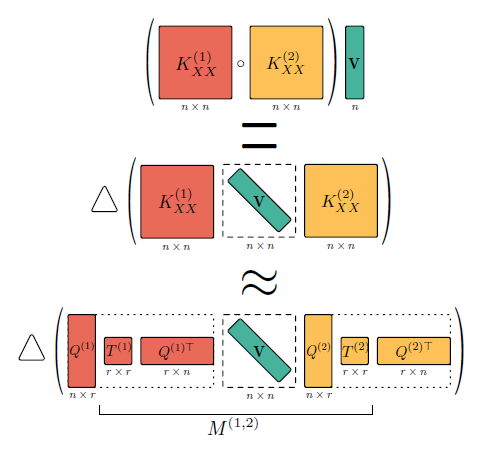
\includegraphics[width=0.4\linewidth]{matrix_vector_multiplication}
     \caption{Figure from \cite{gardner2018product}. Illustration MVMs with the product kernel $K_{X,X}^{1} \circ K_{X,X}^{2}$ }\label{fig:MVM}
\end{figure}

Now, we use the Lancos decomposition (see appendix section (\ref{appendix_lanczos_dec})). In short, it takes a symmetric $n \times n$ $A$ matrix and probe vector $\bm{b}$ and returns a $Q$ and $T$ such that $A \approx Q T Q^t$ with $Q$ orthogonal. The algorithm is exact after $n$ iterations and requires only $1$ MVM per iteration. It has been showed that, by only computing $r < n$ columns of $Q$, an effective low-rank approximation $Q_{\bm{r}} T_{\bm{r}} Q_{\bm{r}}^t$ of $A$ can be obtained. We obtain the following lemma. 

\begin{Lemma}[Time complexity Lanczos decomposition] \label{lemma_time_complexity_lancos_decomposition}
Suppose that MVMs with $K_{X,X}^{(i)}$ can be computed in $O(\mu(K_{X,X}))$ time. Then, the Lanczos decomposition of rank $r$ given by $K_{X,X}^{(i)} \approx Q_{\bm{r}}^{(i)}  (T_{\bm{r}})^{(i)} (Q_{\bm{r}}^{(i)})^{t} $, can be computed in $O(r\mu(K_{X,X}^{(i)}))$ time.
\end{Lemma}

Next, we obtain the following lemma.

\begin{Lemma}[Time complexity of equation  (\ref{Product_kernel_interpol_1})]\label{lemma_time_complexity_matrix_mult}
Suppose that $K_{X,X}^{(1)} = Q_{\bm{r}}^{(1)}  T_{\bm{r}}^{(1)} (Q_{\bm{r}}^{(1)})^{t}$ and $K_{X,X}^{(2)} = Q_{\bm{r}}^{(2)}  T_{\bm{r}}^{(2)} (Q_{\bm{r}}^{(2)})^{t}$ with $Q_{\bm{r}}^{(1)}$,  $Q_{\bm{r}}^{(1)}$ both $n \times r$ matrices and $T_{\bm{r}}^{(1)}$, $T_{\bm{r}}^{(2)}$ both $r \times r$ matrices. Then, equation  (\ref{Product_kernel_interpol_1}) can be computed in $O(nr^2)$ time.
\end{Lemma}

\begin{proof}
A visual representation of the proof can be found in the last image in figure (\ref{fig:MVM}). Both $T_{\bm{r}}^{(1)} (Q_{\bm{r}}^{(1)})^{t}$ and $ Q_{\bm{r}}^{(2)}  T_{\bm{r}}^{(2)}$ can be computed in $O(n r^2)$ time. Multiplying one of the previous two with $D_{\bm{v}}$ takes $O(nr)$ time and multiplying these two matrices together is of order $O(n r^2)$. Hence the $r \times r$ matrix $M = T_{\bm{r}}^{(1)} (Q_{\bm{r}}^{(1)})^{t} D_{\bm{v}} Q_{\bm{r}}^{(2)}  T_{\bm{r}}^{(2)}$ can be computed in $O(n r^2)$ time. We only need the diagonal elements of $K_{X,X}^{(1)} D_{\bm{v}} (K_{X,X}^{(2)})^t$ , hence the necessary outer multiplications only take $O(nr)$ time.  
\end{proof}

Combining lemma (\ref{lemma_time_complexity_lancos_decomposition}) and lemma (\ref{lemma_time_complexity_matrix_mult}), we can compute an approximation of equation  (\ref{Product_kernel_interpol_1}) in $O\left(r \mu(K_{X,X}^{(2)}) +r \mu(K_{X,X}^{(2)}) + r^2n \right)$ time. We can easily extend the previous to product kernels with many components. Given a kernel matrix $ K_{X,X} = K_{X,X}^{(1)} \circ \cdots \circ K_{X,X}^{(d)}$, we define 

\begin{align}
&\tilde{K}_{X,X}^{(1)} = K_{X,X}^{(1)} \circ \cdots \circ K_{X,X}^{\left(\frac{d}{2}\right)} \nonumber \\
&\tilde{K}_{X,X}^{(2)} = K_{X,X}^{\left(\left(\frac{d}{2}\right) + 1\right)} \circ \cdots \circ K_{X,X}^{(d)}. 
\end{align}

Hence, we can write $ K_{X,X} = \tilde{K}_{X,X}^{(1)} \circ \tilde{K}_{X,X}^{(2)}$. We can apply this splitting recursively (we need $O(\log(d)$ merges) and obtain theorem  (\ref{theorem_multi_prod}).

\begin{Theorem}\label{theorem_multi_prod}
Suppose that $ K_{X,X} = K_{X,X}^{(1)} \circ \ldots \circ K_{X,X}^{(d)}$, and that computing a MVM with $K_{X,X}^{(i)}$ can be computed in $O(\mu(K_{X,X}^{(i)}))$ time (assume this is the same for all $i$). Computing a MVM with $K_{X,X}$ requires $O(dr \mu(K_{X,X}^{(i)}) +r^{3} n \log{(d)} + r^2n)$, with $r$ the rank of the Lanczos decomposition as before.
\end{Theorem}

\begin{proof}
We first need the Lanczos decomposition of the $d$ component matrices which takes $O\left(dr\mu(K_{X,X}^{(i)}) \right)$ time. Next, we perform  $O(\log{(d)})$ merges which each takes $O(n d^3)$ time using lemma (\ref{lemma_time_complexity_lancos_decomposition}) and noticing that we now do a matrix matrix multiplication (MMM).  Finally MVMs with $ K_{X,X}$ takes $O(n r^2)$ time. We find that a single MVM with $K_{X,X}$ takes $O(dr \mu(K_{X,X}^{(i)}) +r^{3} n \log{(d)} + r^2n)$ time. 
\end{proof}

Notice that the term $O(dr \mu(K_{X,X}^{(i)}) +r^{3} n \log{(d)})$ represents the construction time of the Lanczos decomposition. Hence, if we store the decomposition further use, any subsequent MVMs with $ K_{X,X}$ takes $O(n r^2)$ time. Now, we use the constructions of section (\ref{section_struct_ker_interpol}) about structured kernel interpolation. We apply the approximation 

\begin{equation}
K_{X,X}^{(i)} \approx W K_{Z,Z} W^t 
\end{equation}
for each component.

\begin{Theorem}
Using the structured kernel interpolation approximation for the components, the time complexity of constructing a rank $r$ Lanczos decomposition and computing a MVM with $ K_{X,X}$ takes 
$O(dr (n + m \log{(m)}) +r^{3} n \log{(d)} + r^2n)$.
\end{Theorem}

\begin{proof}
It follows from the fact that MVMs with $K_{X,X}^{(i)}$ can be computed in $O(n + m \log{(m)})$ exploiting the Toeplitz structure.  
\end{proof}

We now have that the time complexity is linear in dimension, without severely punishing the amount of inducing points,  which is a huge improvement. We call this method SKIP (Structured Kernel Interpolation for Products). However, this section was only a foretaste of what is possible. In the next section, we discuss a whole framework which enables a speed-up of almost all the methods we have seen before. 


\iffalse
Now let us compare the time complexity of the naive approach of section (\ref{section_struct_ker_interpol}) with the more advanced method of this section. 


Let us now use the product kernel structure (see equation (\ref{Functional_Product_first_eq})), which we will exploit in the next section. Let us denote with Hence, using equation (\ref{interpolsation_1d}), we can write

\begin{equation}
k_{X,Z} = \prod\limits_{j=1}^{d} k^{(j)}_{x_j,u_j} \approx \prod\limits_{j=1}^{d} \sum_{i=1}^m w_i k_{\bm{u}_i,\bm{u}_j}^{(j)}.
\end{equation}

\fi

\section{Blackbox Matrix-Matrix Gaussian Process}\label{section_BBMM}

In this section, we follow \cite{gardner2018gpytorch}. We discuss a framework called Blacbox Matrix Matrix (BBMM) inference that can be used as a black-box which performs matrix-matrix multiplications with a kernel matrix and its derivative.  Denoting with $\hat{K}_{X,X} = \tilde{K}_{X,X} + \sigma^2 I$ (also including the exact case), the evidence is given by 

\begin{equation}
l(\bm{\theta} | X, \bm{y}) = \log p(\bm{y}|X) = -\dfrac{1}{2} \bm{y}^t (\hat{K}_{X,X})^{-1} \bm{y} -\dfrac{1}{2} \log |\hat{K}_{X,X}| - \dfrac{n}{2}  \log(2 \pi).
\end{equation}

Using lemma (\ref{appendix_stoch_tr_approx}) in the appendix one can easily find that its derivative towards a hyperparameter $\theta$ is given by

\begin{equation}
\dfrac{dl}{d \theta} = \bm{y}^t (\hat{K}_{X,X})^{-1} \dfrac{d \hat{K}_{X,X}}{d \theta} (\hat{K}_{X,X})^{-1} \bm{y} + \Tr \left( (\hat{K}_{X,X})^{-1} \dfrac{d \hat{K}_{X,X}}{d \theta} \right).
\end{equation}

The calculation of derivative is for example necessary in order to use the Adam algorithm (see appendix section (\ref{appendix_adam})). Hence, in order to train our model, we need fast ways to calculate $(\hat{K}_{X,X})^{-1} \bm{y}$, $\Tr \left( (\hat{K}_{X,X})^{-1} \frac{d \hat{K}_{X,X}}{d \theta} \right)$ and $\log |\hat{K}_{X,X}|$ in an efficient way. Before we can continue with our discussion, we need to say a word about preconditioning on the system $(\hat{K}_{X,X})^{-1} \bm{y}$   (see appendix section (\ref{appendix_preconditioning}) for more information). Now, the preconditioner needs to satisfy two requirements. First, we need to compute the determinant of this preconditioner matrix $P$ since 

\begin{equation}
\log | \hat{K}_{X,X}) | = \log | P^{-1} \hat{K}_{X,X}) | + \log |P|.
\end{equation}

One can calculate $\log | P^{-1} \hat{K}_{X,X}) |$ in a fast way using the CG method which we explain later. Secondly, the calculation of this preconditioner may not dominate the running time, it should only afford a linear time in solves and space. We use the preconditioner called The Pivoted Cholesky Decomposition. We find the preconditioner $\hat{P}_k = (L_k L_k^t + \sigma^2 I)$ with $L_k L_k^t \approx K_{X,X}$. Without going in detail, the preconditioner and its log determinant can be computed and solved in $O(nk^2)$ time. The convergence of CG improves exponentially with the rank of the pivoted Cholesky decompostion for RBF-kernels and the number of CG iterations to accurately estimate $\log | \hat{P}^{-1} \hat{K}_{X,X}) |$ decreases quickly as $k$ increases. 

One uses the Modified Batched Conjugate Gradient (MBCG) Algorithm which performs multiple solves $A^{-1} B = [ A^{-1} \bm{b}_1 , \ldots, A^{-1} \bm{b}_t]$ simultaneously using Matrix-Matrix multiplication (MMM). This algorithm also returns the Lanczos tridiagonalisation matrices associated with each of the solves $\tilde{T}_1, \ldots, \tilde{T}_t$ (see appendix section (\ref{appendix_preconditioning})) which enables fast estimating of the derivative and determinant, which we discuss later. While studying the algorithm, it may be clarifying to compare it with the preconditioned CG algorithm which can be found in the appendix section (\ref{appendix_preconditioning}). We denote with 

\begin{equation}
\dfrac{(R_{(i)} \circ Z_{(i)})^t I}{(D_{(i)} \circ V_{(i)})^t I} =  \left[\dfrac{[R_{(i)}]_1^t [Z_{(i)}]_1 }{[D_{(i)}]_1^t  [V_{(i)}]_1}, \ldots, \dfrac{[R_{(i)}]_t^t [Z_{(i)}]_t }{[D_{(i)}]_t^t  [V_{(i)}]_t} \right]
\end{equation}

and with

\begin{equation}
X_{(i)} + \text{diag}(\bm{\alpha})_{(i)} D_{(i)} = \left[ [X_{(i)}]_1 , \ldots ,[X_{(i)}]_t \right] + \left[[ \bm{\alpha}_{(i)}]_1 [X_{(i)}]_1 ,\ldots , [ \bm{\alpha}_{(i)}]_t [X_{(i)}]_t \right].
\end{equation}

The MBCG algorithm can be found looking at algorithm (\ref{MBCG}). which replaces multiple MVM's with a single MMM allowing to perform multiple solves in parallel which enables GPU acceleration for example. If one is not yet familiar with stochastic trace estimation, it is recommended to read section (\ref{appendix_stoch_trace}) in the appendix.

\begin{algorithm}
\caption{Modified Preconditioned Conjugate Gradient Method (MBCG)}\label{MBCG}
\begin{algorithmic}[1]
\item \textbf{input}: mmm\textunderscore${A}()$, A function for a MMM with $A$
\item \quad $B$, $n \times t$ matrix to solve against
\item \quad $\hat{P}^{-1}()$, a function for preconditioning
\item \textbf{output}: $A^{-1} B, \tilde{T}_1, \ldots, \tilde{T}_t$
\BState \emph{$X_{(0)} = 0$}
\BState \emph{$R_{(0)} = B$ - mmm\textunderscore ${A}(X_{(0)})$}
\BState \emph{$D_{(0)} = Z_{(0)} = \hat{P}^{-1}(R_{(0)})$}
\BState \emph{$\tilde{T}_1, \ldots, \tilde{T}_t = \bm{0}$}
\BState For \emph{$i = 0, \ldots, p$} do :
\State \quad $V_{(i)} = mmm\textunderscore {A}(D_{(i)})$
\State \quad $\bm{\alpha}_{(i)} = \dfrac{(R_{(i)} \circ Z_{(i)})^t I}{{(D_{(i)} \circ V_{(i)})^t I }}$
\State \quad $X_{(i+1)} = X_{(i)} + \text{diag}(\bm{\alpha})_{(i)} D_{(i)}$
\State \quad $R_{(i+1)} = R_{(i)}  - \text{diag} (\bm{\alpha})_{(i)} V_{(j)}$
\State \quad If \emph{ $\forall i : ||R_{(i+1)}||_2 < \text{tolerance}$}, then return $X_{(i+1)}$
\State \quad $Z_{(i+1)} = \hat{P}^{-1}(R_{(i+1)})$
\State \quad $\bm{\beta}_{(i)} = \dfrac{(R_{(i+1)} \circ  Z_{(i+1)})^t I}{ (R_{(i)} \circ Z_{(i)})^t I}$
\State \quad $D_{(i+1)} = Z_{(i+1)}+ \text{diag}(\bm{\beta})_{(i+1)} D_{(i)}$
\State \quad $ \forall j \in (1, \ldots, t) : [\tilde{T}_j]_{i+1,i+1} = \dfrac{1}{[\bm{\alpha}_{(i)}]_j} + \dfrac{[\bm{\beta}_{(i)}]_j}{[\bm{\alpha}_{(i)}]_j}$
\State \quad $ \forall j \in (1, \ldots, t): [\tilde{T}_j]_{i,i+1} = [\tilde{T}_j]_{i+1,i}= \dfrac{\sqrt{[\bm{\beta}_{(i)}]_j}}{[\bm{\alpha}_{(i)}]_j}$
\BState Return \emph{$X_{(i+1)}$} and $\tilde{T}_1, \ldots, \tilde{T}_t$:
\end{algorithmic}
\end{algorithm}
 

Now the preparations are finally done and it is time to do some learning. Let $\bm{z} = (\bm{z}_1, \ldots, \bm{z}_t)^t$ be a vector consisting of $t$ independent samples from a random variable $Z$ with mean $0$ and variance $1$. We execute the MBCG algorithm with input the matrices $\hat{K}_{X,X}$ and $[\bm{y}, \bm{z}_1, \ldots, \bm{z}_t]$ to solve against and the preconditioner  $\hat{P}_k = (L_k L_k^t + \sigma^2 I)$. We obtain $\hat{K}_{X,X}^{-1} \bm{y}$, $\hat{K}_{X,X}^{-1} \bm{z}_i$ and $\tilde{T}_i$ (Lanczos with $p$ iterations and probe vector $\bm{z}_i$) for all $i \in (1, \ldots t)$ as output. Using lemma (\ref{stoch_trace_1}) in the appendix, we find an unbiased estimator of the derivative given by 

\begin{equation}\label{equation_trace}
\Tr \left( \hat{K}_{X,X}^{-1} \dfrac{d\hat{K}_{X,X}}{d\theta} \right) = \mathbb{E} \left[ \bm{z}_i^t \hat{K}_{X,X}^{-1} \dfrac{d\hat{K}_{X,X}}{d\theta} \bm{z}_i \right] \approx \dfrac{1}{t} \sum\limits_{i=1}^t ( \bm{z}_i^t \hat{K}_{X,X}^{-1} ) \left( \dfrac{d\hat{K}_{X,X}}{d\theta} \bm{z}_i \right).
\end{equation}

For the determinant, we use the decompositions $ \tilde{Q}_1 \tilde{T}_1 \tilde{Q}_1^t , \ldots,\tilde{Q}_t \tilde{T}_t \tilde{Q}_t^t $. By using lemma (\ref{stoch_trace_2},\ref{appendix_matrix_lemma}) in the appendix and noticing that $\tilde{Q}_i \bm{z}_i = \bm{e}_1$ (since all but the first colmuns of $Q_i$ are orthogonal to $\bm{z}_i$), we find that 

\begin{align}\label{appendix_stoch_tr_approx}
\log(|K_{X,X}|) &= \Tr (\log (K)) = \mathbb{E}[ \bm{z}_i^t \log (K)\bm{z}_i ] \nonumber \\ &= \mathbb{E}[ \bm{z}_i^t \tilde{Q}_i \log (\tilde{T}_i) \tilde{Q}_i^t  \bm{z}_i ] \approx \dfrac{1}{t} \sum\limits_{i=1}^t e_1^t \log (\tilde{T}_i) e_1.
\end{align}

The last logarithm can be calculated using an eigendecompostion. $\tilde{T}_i = V_i \Lambda_i V_i^{t}$. We find thus that 

\begin{equation}\label{equation_bbmm_einde}
\log(|K_{X,X}|) \approx \sum\limits_{i=1}^t e_1^t V_i \log {(\Lambda)_i} V^{t}_i e_1.
\end{equation} 

Now, we are ready to discuss the time complexity of all our steps. The matrix $\hat{K}_{X,X}$ has a dimension equal to $n \times n$ and all the other matrices used in the MBCG algorithm $(X_i, R_i,V_i,Z_i,D_i, \hat{P}$) have dimension $n \times t$. Hence, besides the matrix $\hat{K}_{X,X}$, we can store everything in $O(nt)$.  All the operations are dominated by the MMM with $\hat{K}_{X,X}$ and a $n \times t$ matrix which takes $O(n^2t)$ time.  

Now, in order to calculate equation (\ref{equation_trace}), one first needs to calculate the single MMM $\frac{d\hat{K}_{X,X}}{d\theta} [ \bm{z}_1, \ldots \bm{z}_t]$. For exact GPRs and sparse approximations, the time complexity of a MMM with the derivative of the kernel is approximately equal to the MMM with the kernel. In the exact case, we have a time complexity of $O(n^2t)$. Next we need $t$ inner products between its columns and the columns of $\hat{K}^{-1}_{X,X}[ \bm{z}_1, \ldots \bm{z}_t]$ which is $O(nt)$. Hence, all of these calculations are dominated by the running time of the MBCG algorithm. 

The dimension of the tridiagonal matrices $\tilde{T}_i$ is equal to $p \times p$. Their eigendecomposition can be computed in $O(p^2)$ time. The computation of equation (\ref{equation_bbmm_einde}) only requires $O(tp)$ additional work. 

Now we can apply and relate this framework with all the methods that we have seen before. For a Cholesky based exact GP-inference we had a time complexity of $(O(n^3))$. However, we have shown that all the previous calculations have a lower asymptotic complexity of $(O(n^2t))$. 

Now, we have that $ \hat{K}_{X,X} \approx ( K_{X,Z} K_{Z,Z}^{-1} K_{Z,X} + \sigma^2 I_n)$ for the SoR approximation. Multiplying this kernel with a $n \times t$ matrix takes only $O(tnm + tm^3)$ time which is again asymptoticaly faster (we can use more inducing points) than the $O(nm^2 + m^3)$ using Cholesky based methods. The discussion for FITC is analogue. 

For the SKI, we use theorem (\ref{SKI_theorem}) and find that a MMM with $\hat{K}_{X,X} \approx ( W K_{Z,Z}^{-1} W^t + \sigma^2 I_n)$ and a $n \times t$ matrix requires $O(tn + tm^2)$. 

In KISS-GP, we exploit the toeplitz structure of $K_{Z,Z}$ and a MMM with a $n \times t$ matrix require only requires $O(tn + tm \log{m})$ time. One can use these framework for training and prediction. We use the BBMM framework for training our data, but predictions are done using the Cholesky decomposition giving more accurate results.

A short extension can of this discussion is given in \cite{wang2019exact}. Let us partition the dataset $X = [X^{(1)}, \ldots, X^{(p)}]$. One can compute the MVM $ \hat{K}_{X,X} \bm{v}$ into partitions by writing 

\begin{equation}
\hat{K}_{X,X} \bm{v} = [ \hat{K}_{\bm{x}^{(1)},\bm{x}} \bm{v}, \ldots,  \hat{K}_{\bm{x}^{(p)},\bm{x}} \bm{v}],
\end{equation}

enabling parallel computations. Having reduced the time complexity of exact Gaussian Processes, one even stated the supremacy over approximate/sparse Gaussian processes. However, remember that sparse Gaussian processes enables very fast predictions.




\chapter{Dessert: Bayesian and Deep Methods}\label{Fully Bayesian GPR}

\section{Fully Bayesian GPR}

In this section, we follow \cite{lalchand2019approximate}. As have been said before, we come across some difficulties when maximising the marginal likelihood  (evidence).  The evidence may be non-convex and when there are many hyperparameters it is prone to overfitting which leads to high variability (Remember f.e. the FITC). First, we give an expression for the predictive posterior going full Bayesian. Next, we discuss some Bayesian techniques  and how they can be used for Gaussian process regression.

As have been said in section (\ref{section_hyperparameter_selection}), we put a prior $p$ over the hyperparameters. We have that 

\begin{equation}
\begin{aligned}
\bm{\theta} &\sim p(\bm{\theta}) \\
\bm{f}| X, \bm{\theta} &\sim \mathcal{N}(\bm{0}, K_{X,X}) \\
\bm{y} | \bm{f} &\sim \mathcal{N}(\bm{f}, \sigma^2 I ).
\end{aligned} 
\end{equation}

We omit the extensive notation including $X$ and $\bm{x}^{\ast}$. By conditioning on the hyperparamters, we find that the predictive distribution is given by

\begin{equation}
p(\bm{f}^{\ast} | \bm{y} ) = \int p(\bm{f}^{\ast} | \bm{y}, \bm{\theta} ) p (\bm{\theta} | \bm{y})  d \bm{\theta}
\end{equation}

Now, like before, we condition over $\bm{f}$ and find that 

\begin{align}
p(\bm{f}^{\ast} | \bm{y} ) &= \int \int p(\bm{f}^{\ast} | \bm{f}, \bm{y} ,  \bm{\theta}) p(\bm{f} ,  \bm{\theta}| \bm{y} ) d \bm{f} d\bm{\theta} \nonumber \\
 &= \int  \int p(\bm{f}^{\ast} | \bm{f}, \bm{y} ,  \bm{\theta}) p(\bm{f} | \bm{y} ,  \bm{\theta}) p( \bm{\theta}| \bm{y} )d \bm{f} \bm{d \theta}.
\end{align}

Notice that for the inner integral 

\begin{equation}
p (\bm{f}^{\ast} | \bm{y}, \bm{\theta}) = \int  p(\bm{f}^{\ast} | \bm{f}, \bm{y} ,  \bm{\theta}) p(\bm{f} | \bm{y} ,  \bm{\theta}) d \bm{f}.
\end{equation}

This is equal to equation (\ref{GPR_Bayesian_2}), (were we used a bit of a different notation which was more appropriate at that moment) or equation \ref{integraal})). We proved that this is equal to (\ref{GPR_Bayesian_3}) and thus find that 

\begin{equation}
p (\bm{f}^{\ast} | \bm{y}, \bm{\theta}) = \mathcal{N}(K_{\bm{x}^{\ast}, \bm{x}}(K_{\bm{x}, \bm{x}} + \sigma^2 I)^{-1} \bm{y} , K_{\bm{x}^{\ast}, \bm{x}^{\ast}} - K_{\bm{x}^{\ast}, \bm{x}} (K_{\bm{x}, \bm{x}} + \sigma^2 I)^{-1} K_{ \bm{x},\bm{x}^{\ast}})
\end{equation}

In the chapter about approximate methods, we used some different expressions for this predictive distribution using inducing points (see equation (\ref{approximate_llh})). For both methods, one can say that we integrate $\bm{f}$ out analytically. Thus we know the expressions for $ p( \bm{f}^{\ast} | \bm{y}, \bm{\theta})$ and write

\begin{equation}\label{full_bayesian}
p (\bm{f}^{\ast} | \bm{y} ) = \int p( \bm{f}^{\ast} | \bm{y}, \bm{\theta}) p (\bm{\theta} | \bm{y} ) d \bm{\theta} \approx \dfrac{1}{M} \sum\limits_{j=1}^{M} p( \bm{f}^{\ast} | \bm{y} , \bm{\theta}_j)  \quad \bm{\theta}_j \sim p(\bm{\theta}|\bm{y}).
\end{equation}

Since the resulting integral is intractable. However, we find the posterior predictive distribution if we can sample $\bm{\theta}_j $ with distribution $p(\bm{\theta}|\bm{y}) \propto p(\bm{y}| \bm{\theta}) p(\bm{\theta})$ . As has been said before, we expect better predictions since that optimisation of the evidence often results in an inferior local optimum and is prone to overfitting. However, we now need to solve a sum of predictive distributions over the data with different hyperparameters every time. This results in a predictive time complexity $M$ times worse than before.

We discuss two different cases. First, one can for example use the MAP estimator (see appendix section (\ref{Appendix_map})) for $\bm{\theta}$ and the calculation of the sum is not necessary anymore. However, one loses the information concerning the uncertainty of the estimations since the map estimator is a point. Next, one can sample these hyperparameters and calculate equation (\ref{full_bayesian}). Although there are a lot of sampling algorithms, we focus on Markov Chain Monte Carlo sampling (MCMC) (see appendix section (\ref{appendix_mcmc})). Denote with $\hat{K}_{X,X} = \tilde{K}_{X,X} + \sigma^2 I_n$ (also including the exact case). The computational cost of these sampling schemes are dominated by the calculation of $p(\bm{y}|\bm{\theta}) \sim \mathcal{N} (\bm{0}, \hat{K}_{X,X})$ (the evidence), which is equal to 

\begin{equation}\label{log_marg_ind_input}
\text{log}p(\bm{y}|\bm{\theta}) = -\dfrac{1}{2} \text{log}|\hat{K}_{X,X}| - \dfrac{1}{2} \bm{y}^t (\hat{K}_{X,X}) \bm{y} - \dfrac{n}{2} \log{(2\pi)}.
\end{equation}

Hence, we are actually dealing with the same problem as before, which was the inversion and the calculation of the determinant of the covariance matrix with has an $O(n^3)$ time complexity for exact GPR and $O(n m^2 +m^3)$ for sparse approximations. Hence, inducing point methods can come at handy reducing the time complexity. We use Metropolis Hasting and an improvement of the Hamiltonian Monte Carlo (HMC) called the No U-Turn Sampler (NUTS). More information can be found in the appendix section (\ref{appendix_mcmc}). 

In a lot of papers like \cite{modelscomparative} and \cite{murray2010slice}, one treats the underlying function values $\bm{f}$ as latent variables and one thus also samples $\bm{f}$. We will not elaborate on this in this section although variants of MH, HMC and slice sampling have been specifically proposed for sampling $\bm{f}$ in these papers. Interested readers are encouraged to read the next section, were we discuss a method sampling from the optimal variational posterior. In the code, we merely focus on sampling $\bm{\theta}$.  For the Metropolis-Hastings algorithm we can for example take a multivariate Gaussian as proposal distribution. We also use NUTS (extension of HMC) in order to sample from  $p(\bm{\theta}|\bm{y}) \propto p(\bm{y}| \bm{\theta}) p(\bm{\theta})$.



\section{Bayesian Variational Method}\label{advanced}

This section and the next  are merely added for completeness. We discover connections with the previous methods and try to obtain more tools concerning Gaussian Process Regression. However, all the methods we discuss from now on will not be included in our data study which means these parts can be skipped. We also omit a lot of the technical details. We begin with a Bayesian approach for variational Gaussian processes discussed in \cite{hensman2015mcmc}). 

Like in the previous section, we start with equation (\ref{integraal})
and equation (\ref{approximate_llh}). However, we do not condition further and use the notation $q(\bm{u}, \bm{\theta})$. We find that

\begin{align}
p(\bm{f}^{\ast} | \bm{y} ) &= \int \int p(\bm{f}^{\ast} | \bm{f}, \bm{y} ,  \bm{\theta}) p(\bm{f} ,  \bm{\theta}| \bm{y} )  d\bm{\theta}d \bm{f} \\
q(\bm{f}^{\ast}) &= \int \int p(\bm{f}^{\ast} | \bm{u}, \bm{\theta}) q(\bm{u} ,  \bm{\theta} ) d \bm{\theta} d \bm{u}.
\end{align}

Notice that $\bm{f}, \bm{u}, \bm{\theta}$ are free parameters of the model. We mimic the calculations of equation (\ref{variational}) which are actually the same. In the variational framework we always want to minimise the KL-divergence between the approximate and the true posteriors which is given by

\begin{equation}
0 \geq \mathcal{K} = -\text{KL} [q(\bm{f}, \bm{u}, \bm{\theta}) || p(\bm{f}, \bm{u}, \bm{\theta} |\bm{y} )] = \mathbb{E}_{q( \bm{f}, \bm{u}, \bm{\theta}) } \left[  \log \left( \dfrac{p(\bm{f}, \bm{u}, \bm{\theta}| \bm{y})}{ q(\bm{f}, \bm{u}, \bm{\theta})}\right) \right] .
\end{equation}

By simplifying the fracture and by conditioning, we can rewrite this expression as

\begin{equation}
\mathcal{K} = \mathbb{E}_{q( \bm{f}, \bm{u}, \bm{\theta}) } \left[ \log \left( \dfrac{ p(\bm{y}|\bm{f}, \bm{u}, \bm{\theta}) p(\bm{u}|\bm{\theta}) p(\bm{\theta})}{q(\bm{u}, \bm{\theta})} \right)  \right] - \log{ (p(\bm{y})}).
\end{equation}

We denote with $C$ an intractable constant normalising the optimal variational distribution. Including this constant, writing down the expectation and some conditioning we find that 

\begin{equation}
\mathcal{K} = - \text{KL} \left[ q(\bm{u}, \bm{\theta}) || \dfrac{p(\bm{u}|\bm{\theta}) p(\bm{\theta}) \exp \left( \mathbb{E}_{p(\bm{f}|\bm{u}, \bm{\theta})} [\log{(p(\bm{y}|\bm{f},\bm{u}, \bm{\theta})}] \right) }{C} \right] - \log{(C)} + \log{(p(\bm{y})}). 
\end{equation}

It may be interesting to compare this equation and the $\mathcal{L}_2$ bound (equation \ref{l2bound}). By omitting the $\bm{\theta}$ parameter and the constant $C$, the KL term is the same expression.  By minimising the KL-divergence we find that the optimal variational distribution is

\begin{equation}
\log{( \hat{q}(\bm{u},\bm{\theta})}) =  \mathbb{E}_{p(\bm{f}|\bm{u}, \bm{\theta})} [\log{(p(\bm{y}|\bm{f}, \bm{u}, \bm{\theta})}] + \log{(p(\bm{u}|\bm{\theta}))} + \log{(p(\bm{\theta}))} - \log{(C)}. 
\end{equation}

The computation of this expression $O(nm^2 +m^3)$ but it factorises across the data enabling scalability by using batches. We make a small detour following \cite{murray2010slice}. The variables $\bm{u}$ and $\bm{\theta}$ are strongly coupled and alternately fixing these variables will not work. We propose a reparametrisation making the parameters independent under the prior.  We draw a vector $\bm{v} \sim \mathcal{N}(\bm{0}, I_m)$. Doing a Cholesky decomposition $K_{Z,Z} = RR^t$, we find that $\bm{u} = R \bm{v}$. Hence, we can rewrite the optimal variational distribution 

\begin{equation}
\log{( \hat{q}(\bm{u},\bm{\theta})} =  \mathbb{E}_{p(\bm{f}|\bm{u} = R \bm{v})} [\log{(p(\bm{y}|\bm{f},\bm{u}, \bm{\theta})}] + \log{(p(\bm{v})}) + \log{(p(\bm{\theta}))} - \log{(C)}. 
\end{equation}

Now, for fixed $\bm{v}$, we can choose to update $\bm{\theta}$ which implicitly updates $\bm{u}$. In \cite{hensman2015mcmc}, one discusses a method using HMC sampling the $\bm{v}$ and $\bm{\theta}$ jointly. 

\section{Deep methods for Gaussian processes}


Deep learning is a family of machine learning methods based on neural networks. Readers which are not yet familiar with neural networks can read \cite{nielsen2015neural} which is a very basic yet understandable introduction. For completeness, we give a short outline of deep methods for Gaussian Processes again omitting details and practical implementations. 


\begin{figure}[!htb]
     \centering
     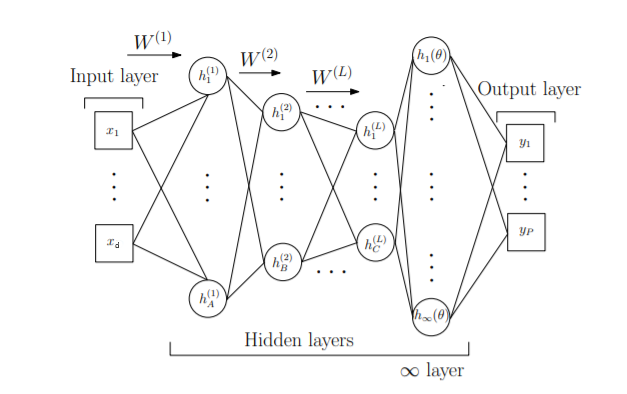
\includegraphics[width=0.4\linewidth]{plot_deep_gpr}
     \caption{Figure from \cite{wilson2016deep}. Deep Kernel Learning also including multidimensional outputs}\label{fig:deep_gpr1.1}
\end{figure}

In \cite{wilson2016deep}, one introduces GP models that use kernels parametrized by neural networks called deep kernel learning (DKL). Starting from a base kernel $k(\bm{x}_i, \bm{x}_j | \bm{\theta})$ we transform the input as 

\begin{equation}
k(\bm{x}_i, \bm{x}_j | \bm{\theta}) \rightarrow k(g(\bm{x}_i, \bm{w}), g(\bm{x}_j, \bm{w})| \bm{w}, \bm{\theta}),
\end{equation}

where $g(\bm{x}, \bm{w})$ is a non-linear mapping given by a deep architecture capturing hierarchical structure and non-stationary. The structure of the model for deep kernel learning can be found in figure (\ref{fig:deep_gpr1.1}). It is a gaussian process with $d$-dimensional inputs trough $L$ hidden layers followed by a hidden layer with infinite basis functions including the base kernel hyperparameters $\bm{\theta}$. 


The parameters $\bm{\theta}$ and $\bm{w}$ can be learned by maximising the evidence (equation \ref{log_marg_ind_input}). Of course, inducing points methods like SoR, FITC and KISS-GP are also possible by replacing the covariance matrix and modifying the evidence. 

One year later, one proposed in \cite{wilson2016stochastic} a method for deep kernel learning using a stochastic variational approach which allows stochastic training spaces but the paper focusses on classification.

In \cite{damianou2013deep}, one introduces the concept of Deep Gaussian Processes (DGP). Now, a DGP defines a prior recursively on $\bm{f}^1, \ldots, \bm{f}^L$. The prior is an independent GP in each dimension. The outputs at layer $l$ are $\bm{f}^l$ and the inputs are $\bm{f}^{l-1}$ with some Gaussian noise included. In \cite{damianou2013deep}, one forces the the input of each layer to be independent of the output of the previous layer. We discuss the paper of \cite{salimbeni2017doubly}, not forcing independence or Gaussian form between the layers, sacrificing analytical tractability. We denote with $Z^{l}$ and $\bm{u}^l$ the inducing locations and values at layer $l$. A DGP has joint density 

\begin{equation}
p(\bm{y}, \{ \bm{f}^l, \bm{u}^l \}^L_{l=1}) = \prod\limits_{i=1}^n p(\bm{y}_i|\bm{f}_i^L)\prod\limits_{i=1}^L p(\bm{f}^l|\bm{u}^l,\bm{f}^{l-1}, Z^{l-1})p(\bm{u}^l, Z^{l-1}),
\end{equation}

with $\bm{f}^0 = X$. They propose a posterior having the property to maintain the exact model conditioned on $U^l$, that is factorized between layers (and dimension) and that $q(U^l)$ is a Gaussian with mean $\bm{m}^l$ and variance $S^l$. Hence, the posterior has the following form

\begin{equation}
q( \{ \bm{f}^l, U^l  \}_{l=1}^{L} ) = \prod\limits_{l=1}^{L} p(\bm{f}^l | \bm{u}^l , \bm{f}^{l-1}, Z^{l-1} ) q (\bm{u}^l).
\end{equation}

Next, we can again find the evidence lower bound minimising this approximate and the true posterior. We have already done similar calculations two times thus we omit it here. We find that the evidence lower bound of this DGP is 

\begin{equation}
\begin{aligned}
\mathcal{L}_{DGP} &= - \text{KL} [q( \{\bm{f}^l, \bm{u}^l \}_{l=1}^L )|| p( \bm{y}, \{\bm{f}^l , \bm{u}^l \}^{L}_{l=1} )] \\
&= \sum\limits_{i=1}^{n} \mathbb{E}_{q(\bm{f}_{i}^L}[ \log (p(\bm{y}_i | \bm{f}_i^L)] - \sum\limits_{l=1}^L \text{KL}[ q(\bm{u}^l) || p(\bm{u}^l, Z^{l-1} ].
\end{aligned}
\end{equation}

We can approximate the equation using Monte Carlo sampling from $q(\hat{\bm{f}}_i^L)$ which we discuss in a second. Notice that the bound factorises over the data, enabling scalability through batching data.

Now use equation (\ref{variational_pred}) (replace $\bm{f}^{\ast}$ by $\bm{f}$) and denote $q(\bm{f}|\bm{m}, S,X,Z ) = \mathcal{N}(\bm{f}| \bm{\tilde{\mu}}, \tilde{\Sigma})$. After marginalising the inducing values of each layer, we find that

\begin{equation}
q (\{ \bm{f}^l \}_{i=1}^L) = \prod\limits_{i=l}^L q(\bm{f}^l | \bm{m}^l, S^l, F^{l-1}, Z^{l-1}) =  \prod\limits_{i=1}^L \mathcal{N}(\bm{f}^l | \bm{\tilde{\mu}} , \tilde{\Sigma}).
\end{equation}

In \cite{salimbeni2017doubly}, one uses a non-zero mean function for the inner layers. Notice that $\bm{f}^{L}_i$ only depends on $\bm{f}_i^{L-1}$ which only depends on $\bm{f}_i^{L-2}$ and so on. Since, $q (\{ \bm{f}^l \}_{i=1}^L)$ is a fully factorised Gaussian we can apply the reparamisation trick (see \cite{kingma2015variational}) sampling only using univariate Gaussians. Hence we receive samples $\hat{\bm{f}}_i^l \sim q(\bm{f}_i^l| \bm{m}^l, S^l, \bm{f}_i^{l-1} , Z^{l-1})$ 

Next, to obtain the density over $\bm{f}^{(L) {\ast}}$, we use the Gaussian mixture

\begin{equation}
q(\bm{f}^{(L) {\ast}}) = \dfrac{1}{M} \sum\limits_{j=1}^M q(\bm{f}^{(L) {\ast}} | \bm{m}^L, S^L, \bm{f}^{(L-1) \ast}_{(j)}, Z^{L-1}).
\end{equation}

More information and further model details can be found in the source.







\chapter{Gaussian Process Regression in Finance} \label{GPR_in finance}

In this section, we try to train a model which is able to price options. All the simultations were done on an Asus computer with Intel core i7 processor, 8GB ram and a Nividia Geforce 920mx graphic card. It is important to take into account possible background processes which could have slow down some calculations.

Before continuing, some special attention is given to  \cite{abadi2016tensorflow},  \cite{salvatier2016probabilistic} and \cite{gardner2018gpytorch}, which represent the packages tensorflow, pymc3 and gpytorch in python. When one of these packages is used, we use the abbreviations `tf', `pym' and `gpy'. The code and datasets which are used for the data study can be found on github: https://github.com/2290Veusseleir/Thesis-Machine-Learning-In-Finance.

We apply the parameter space of the models which was used in \cite{de2018machine}, although a bigger or smaller space is also possible. We use two measures quantifying the quality of pricing/prediction. The first quantifies the maximum absolute error and the second the average absolute error

\begin{align}
\text{MAE} &= \max \left[ |\bm{y}_i - \bm{f}^{\ast}_i |, i \in (1,\ldots, n) \right]  \\
\text{AAE} &= \dfrac{1}{n} \sum\nolimits_{i=1}^{n} | \bm{y}_i - \bm{f}^{\ast}_i | .
\end{align}

We start with pricing vanilla options in the Heston model. The parameter ranges used for training and validation can be found in table (\ref{table_vanilla's}). All the parameters are sampled uniformly excepted $\sigma$ and $v_0$, which are sampled from a bounded exponential distribution to incorporate more small volatilities in the training set. For training, notice that we shrink the parameter space a little in order to avoid the edges.

\begin{table}\centering 
\begin{tabular}[t]{lccc}\toprule
            &   Product/Market  &  Heston &  VG   \\ \midrule
            Training set &&& \\\addlinespace
 & $K: 40 \% \rightarrow 160\%$ & $\kappa: 1.4 \rightarrow 2.6$ &  $\sigma: 0.05 \rightarrow 0.45$ \\\addlinespace
			   & $T: 11M \rightarrow 1Y$      &  $\rho: -0.85 \rightarrow -0.55$   &  $\nu: 0.55 \rightarrow 0.95$     \\\addlinespace
			   & $r: 1.5\% \rightarrow 2.5\%  $   & $\theta: 0.45 \rightarrow 0.75$     &  $\theta:  -0.35 \rightarrow -0.05$     \\\addlinespace
			   & $q: 0 \%  \rightarrow 5 \%$    & $\eta: 0.01 \rightarrow 0.1$     &       \\\addlinespace
			   &      &  $v_0: 0.01 \rightarrow 0.1$   &       \\\addlinespace
			    Test set &&& \\\addlinespace
 & $K: 50 \% \rightarrow 150\%$ & $\kappa: 1.5 \rightarrow 2.5$ & $\sigma: 0.1 \rightarrow 0.4$  \\\addlinespace
			   & $T: 11M \rightarrow 1Y$      &  $\rho: -0.8 \rightarrow -0.6$   &  $\nu: 0.6 \rightarrow 0.9$     \\\addlinespace
			   & $r: 1.5\% \rightarrow 2.5\%  $   & $\theta: 0.5 \rightarrow 0.7$     &  $\theta:  -0.3 \rightarrow -0.1$    \\\addlinespace
			   & $q: 0 \%  \rightarrow 5 \%$    & $\eta: 0.02 \rightarrow 0.1$     &       \\\addlinespace
			   &      &  $v_0: 0.02 \rightarrow 0.1$   &       \\\bottomrule
\end{tabular}
\caption{Parameter ranges training and validation vanilla options}\label{table_vanilla's}
\end{table}

We are ready to compare the different methods we discussed. First, pay attention to the increase in computation time for the different methods when increasing the amount of data/inducing points and compare them with the theoretical time complexities. Next, notice that we can almost exactly calculate the values of vanillas in the Heston (and Variance Gamma model). The only approximation we make is the Simpson's rule to evaluate an integral (see appendix section (\ref{Fast_Fourrier_transform})). Hence, we predict using noise-free observations, which means that we need to take the Gaussian noise variance $\sigma^2$ as close as possible to zero. Doing this, we can encounter problems concerning the inversion of the covariance matrix $K$ of the GPR. We also calculate the MAE and the AAE for all models, quantifying their predictive ability. Our main goal was to calculate the price of an option faster. Hence, the prediction time is also very important. 


We try to train $1000$, $4000$ and (if feasible) $10000$ points. Next, we predict $1000$ new data points and calculate their MAE and AAE. We take the maximum of zero and the predicted value since the price of an option can not be negative. We always mention the amount of inducing points we used. A clear scheme of all the models and abbreviations we discussed can be found in chapter (\ref{sum_conc}). We programmed $14$ different regression models, $3$ different financial models and $4$ kinds of options in python. Comparing all these regression models using different options and financial models will create a mess. Hence, we made a selection discussing the most promising and important regression models.

Models we will not discuss are FITC and VFE with training the locations of the inducing points by optimising the evidence, SKIP, SVG using gpytorch and exact GPR and VFE going full Bayesian. We did not include the SKIP method since it suffers from tuning and stability issues using big ill-conditioned matrices due to the extensive use of the Lanczos decomposition in training and predicting. For small datasets, we do not encounter problems using this method. We also do not include the full Bayesian methods in our competitive data study since they are too slow. However using these methods, we obtain information concerning the uncertainties of the hyper-parameters. Some beautiful plots using the full Bayesian methods for vanilla calls in the Heston model are given at the end of this section.  

We omit the pricing of options using the Variance Gamma model and the MAE and AAE of the training set. Interested readers can run and study the code for these cases themselves. Notice that we need to make a lot of assumptions i.e. the amount of iterations and the learning rate for numerical/stochastic methods. This means that results can differ when you run the code yourself.

First, we try to calculate the options using the FFT algorithm (which we did not parallelize). Then we train a polynomial regression (PR) model which can be seen as our point of comparison. Notice that the function $(S_T - K)^{+}$ (see equation (\ref{price_vanillas})), has a hockey stick shape if we plot it against $K$. Since the strike is a very important parameter, a quadratic model can give decent results. Next, we train the standard GPR model without any modifications and a fixed noise variance $\sigma^2$. Subsequently, we train the FITC and VFE using k-means for the inducing points and a fixed noise variance $\sigma^2$, which appears to be very good approximation models. In these implementations we do not further train the inducing points and the noise variance. Thereafter, we train the SVG-model which initialises the inducing points with k-means and we train them further. We again fix the noise variance. We continue with training the standard GPR and VFE model using BBMMs and training basic GPR and VFE with MAP determining the place of the inducing points using k-means but training the noise variance. The outcomes can be found in table (\ref{Result_Heston_Vanilla_Call}). Ignoring the outcomes from the FFT and polynomial regression, the best results are in bold. 

We first discuss the exact GPR models. For these models, we obtain very accurate predictions. However, the time complexity of $O(n^3)$ gives us problems using large datasets. Using the standard GPR model using BBMM, there is a trade-off between the computation time $O(n^2)$ and some accuracy. However, the BBMM enables the use of more data points, and very accurate predictions can be achieved. The prediction time for the exact methods is $O(n)$. The very fast prediction time of $O(m)$ is the main advantage of using inducing point methods. Since the time complexity of standard inducing point methods is still $O(nm^2 +m^3)$, it may be appropriate to use stochastic techniques or to use the BBMM framework decreasing the computation time dramatically for a presumably small increase in prediction error. The methods using MAP give somewhat the same results as the corresponding exact GPR and sparse methods. The differences are due to the use of a prior for the hyperparameters, the training of the noise variance and the different implementation. 


\begin{table}\centering 
\begin{tabular}[t]{lcccc}\toprule
            &   Training Time  &  Prediction time  &  MAE & AAE   \\ \midrule
FFT(n=1000/4000/10000)    &/ & $5.1165$ &  $0$  &  $0$    \\\addlinespace
PR(n=1000)   & $0.0076$ & $0.0022$    & $0.0272$ &  $0.0058$     \\\addlinespace
PR(n=4000)   &  $0.0187$  & $0.0024$ & $0.0284$ &  $0.0056$   \\\addlinespace
PR(n=10000)	  &   $0.0293$ & $0.0025$ & $0.0273$ & $0.0056$     \\\addlinespace
\qquad \qquad \qquad \qquad \qquad ---	  &   --- & --- & --- & ---     \\\addlinespace
GPR(n=1000)   &  $7.9999$  & $0.0332$ & $0.0054$ &  $0.00077$   \\\addlinespace
GPR(n=4000)   &  $507.78$  & $0.1354$  & $0.0030$ & $0.00040$    \\\addlinespace
FITC(n=1000)(m=200)  & $10.722$ & $\bm{0.0062}$   & $0.0136$ &  $0.0027$     \\\addlinespace
FITC(n=4000)(m=200)   & $53.628$   & $0.0064$ & $0.0132$ &  $0.0026$   \\\addlinespace
FITC(n=4000)(m=400)	 & $129.58$   & $0.0120$ & $0.0125$ & $0.0023$    \\\addlinespace
VFE(n=1000)(m=200)  & $10.0022$ & $0.0062$   & $0.0090$ & $0.0017$  \\\addlinespace
VFE(n=4000)(m=200)   & $68.471$ &  $0.0082$   & $0.0089$ & $0.0016$     \\\addlinespace
VFE(n=4000)(m=400)	 & $148.48$ &  $0.0113$   & $0.0102$ & $0.0017$    \\\addlinespace
SVG(n=1000)(m=200)(tf)  & $5.7177$    & $0.0084$ &$0.0109$  &  $0.0020$   \\\addlinespace
SVG(n=4000)(m=200)(tf)  & $10.9812$   & $0.0085$ & $0.0115$ & $0.0019$    \\\addlinespace
SVG(n=10000)(m=400)(tf)	  & $49.520$   & $0.01734$  & $0.0100$ &  $0.0016$   \\\addlinespace
GPR(n=1000)(BBMM)(gpy)  & $\bm{2.1939} $  & $0.0415$ & $0.0058$ & $0.00095$    \\\addlinespace
GPR(n=4000)(BBMM)(gpy)  & $21.433$   & $0.1331$ & $0.0055$ & $0.00074$    \\\addlinespace
GPR(n=10000)(BBMM)(gpy)  & $138.54$   & $0.2965$  & $0.00358$ &     $0.00037$ \\\addlinespace
VFE(n=1000)(m=200)(BBMM)(gpy)  & $5.3466$   & $0.0083$ & $0.0115$ & $0.0021$    \\\addlinespace
VFE(n=4000)(m=200)(BBMM)(gpy)  &  $24.525$  & $0.0074$ & $0.0109$ &  $0.0018$   \\\addlinespace
VFE(n=10000)(m=400)(BBMM)(gpy) &$104.27$ & $0.01289$ & $0.01386$ &  $0.0017$  \\\addlinespace
GPR(n=1000)(MAP)(pym)  & $25.421$   & $0.0348$  & $0.0053$ &  $0.00078$   \\\addlinespace
GPR(n=4000)(MAP)(pym)  & $1005.2$   & $0.1903$ & $\bm{0.0021}$ &  $\bm{0.00027}$   \\\addlinespace
VFE(n=1000)(m=200)(MAP)(pym)  &  $16.8254$  & $0.0070$ & $0.0131$  & $0.0024$    \\\addlinespace
VFE(n=4000)(m=200)(MAP)(pym)  & $83.927$   & $0.0072$ & $0.0126$ & $0.0023$    \\\addlinespace
\\\bottomrule
\end{tabular}
\caption{Training and predicting vanilla calls using the Heston model}\label{Result_Heston_Vanilla_Call}
\end{table}

In the next data study we try to train models which are able to predict DOBP options using the Heston model. The corresponding parameter ranges can be found in table (\ref{table_DOBP}). Often, algorithms pricing these derivatives use Monte-Carlo simulation and are thus very slow. We take the opportunity to test how our models cope with noisy data and outliers. In our training set, we only simulate $1000$! different paths with time steps of $1$ day. Hence, the value of the DOBP corresponding to this simulation will be quite noisy. Next, we test our model using $100$ accurate test points. We price them simulating $100000$ different paths with time steps of $1$ day.  The results can be found in table (\ref{dobp_outcomes}). 

Notice that pricing using Monte-Carlo simulations takes a very long time. We again omitted any form of parallelisation. Hence, using GPR for pricing difficult/exotic options can be very advantageous. Predicting using VFE with the BBMM framework is $9339.3 / 0.00032 = 29185312.5$  times faster than pricing the option with MC simulations. Using less noisy data, all the models obtain better prediction values (which we do not discuss). 

Equally important, this simulation tests how our models can handle noisy data. Although the difference between computation time between exact and approximate models stay the same, the difference between their predictive ability is less severe as before.  However, for FITC we stumbled on some problems tuning the noise variance parameter. For a discussion comparing FITC and VFE and their shortfalls, see the end of section (\ref{var_regr}). Using SVG and VFE with BBMM, we obtain fast and accurate predictions with fast training. 

\begin{table}\centering 
\begin{tabular}[t]{lcc}\toprule
            &   Product/Market  &  Heston   \\ \midrule
            Training set && \\\addlinespace
 & $K: 40 \% \rightarrow 160\%$ & $\kappa: 1.4 \rightarrow 2.6$  \\\addlinespace
			   & $T: 11M \rightarrow 1Y$      &  $\rho: -0.85 \rightarrow -0.55$       \\\addlinespace
			   & $r: 1.5\% \rightarrow 2.5\%  $   & $\theta: 0.35 \rightarrow 0.75$         \\\addlinespace
			   & $q: 0 \%  \rightarrow 5 \%$    & $\eta: 0.01 \rightarrow 0.16$            \\\addlinespace
			   &  $H: 0.55 \rightarrow 0.99$      &  $v_0: 0.01 \rightarrow 0.16$          \\\addlinespace
			    Test set && \\\addlinespace
 & $K: 50 \% \rightarrow 150\%$ & $\kappa: 1.5 \rightarrow 2.5$  \\\addlinespace
			   & $T: 11M \rightarrow 1Y$      &  $\rho: -0.8 \rightarrow -0.6$       \\\addlinespace
			   & $r: 1.5\% \rightarrow 2.5\%  $   & $\theta: 0.4 \rightarrow 0.7$       \\\addlinespace
			   & $q: 0 \%  \rightarrow 5 \%$    & $\eta: 0.02 \rightarrow 0.16$           \\\addlinespace
			   &      &  $v_0: 0.02 \rightarrow 0.16$         \\\bottomrule
\end{tabular}
\caption{Parameter ranges training and validation for DOBP options }\label{table_DOBP}
\end{table}


\begin{table}\centering 
\begin{tabular}[t]{lcccc}\toprule
            &   Training Time  &  Prediction time &  MAE & AAE   \\ \midrule
MC(n=1000/4000/10000)    &/ & $9339.3$ &  $0$  &  $0$    \\\addlinespace
PR(n=1000)   & $0.0102$ &  $0.0026$   & $0.0403$ &   $0.0087$   \\\addlinespace
PR(n=4000)   & $0.0199$ &  $0.0024$   & $0.0399$ & $0.0082$     \\\addlinespace
PR(n=10000)	  & $0.5273$ & $0.0032$    & $0.0397$ &  $0.0084$     \\\addlinespace
\qquad \qquad \qquad \qquad \qquad ---	  &   --- & --- & --- & ---     \\\addlinespace
GPR(n=1000)   & $7.7419$ &  $0.0056$   & $0.0248$ &  $0.0042$   \\\addlinespace
GPR(n=4000)   & $253.23$  &  $0.0149$   & $0.0221$  &  $0.0029$    \\\addlinespace
FITC(n=1000)(m=200)  & $11.237$ & $0.00048$    & $0.0265$ & $0.0055$  \\\addlinespace
FITC(n=4000)(m=200)   & $51.248$ & $0.00074$    & $0.0551$ &  $0.0081$   \\\addlinespace
FITC(n=4000)(m=400)	 & $106.68$ &  $0.00070$   & $0.0462$  &  $0.0062$   \\\addlinespace
VFE(n=1000)(m=200)  & $11.075$ & $0.00048$    & $0.0265$ & $0.0055$  \\\addlinespace
VFE(n=4000)(m=200)   & $82.402$  & $0.00050$    & $0.0232$ &  $0.0050$   \\\addlinespace
VFE(n=4000)(m=400)	 & $165.68$  & $0.00108$    & $0.0221$ & $0.0037$    \\\addlinespace
SVG(n=1000)(m=200)(tf)  & $9.6830$ & $0.00081$    & $0.0286$ & $0.0049$  \\\addlinespace
SVG(n=4000)(m=200)(tf)  & $15.3821$ & $0.00058$   & $0.0222$ & $0.0046$  \\\addlinespace
SVG(n=10000)(m=400)(tf)	  & $45.084$  & $0.0017$    & $0.0178$ & $0.0029$  \\\addlinespace
GPR(n=1000)(BBMM)(gpy)  & $\bm{2.6267}$  & $0.0030$    & $0.0501$ &  $0.0040$     \\\addlinespace
GPR(n=4000)(BBMM)(gpy)  & $25.860$  & $0.0405$    & $0.0242$ & $0.0031$  \\\addlinespace
GPR(n=10000)(BBMM)(gpy)  & $347.99$ & $0.0310$    & $0.0202$ & $0.0026$  \\\addlinespace
VFE(n=1000)(m=200)(BBMM)(gpy)  & $3.2922$ & $\bm{0.00032}$     & $0.02802$ &    $0.0056$ \\\addlinespace
VFE(n=4000)(m=200)(BBMM)(gpy)  & $30.989$ & $ 0.00049$    & $0.0240$ &    $0.0047$ \\\addlinespace
VFE(n=10000)(m=400)(BBMM)(gpy)  & $112.05$ &  $0.00095$  & $0.0221$ & $0.0033$  \\\addlinespace
GPR(n=1000)(MAP)(pym)  & $23.885$  &  $0.0028$   & $0.0258$ & $0.0033$  \\\addlinespace
GPR(n=4000)(MAP)(pym)  & $868.19$ & $0.2658$    & $\bm{0.0216}$ & $\bm{0.0025}$   \\\addlinespace
VFE(n=1000)(m=200)(MAP)(pym)  & $18.401$ & $0.00033$    & $0.0298$  &   $ 0.0055$ \\\addlinespace
VFE(n=4000)(m=200)(MAP)(pym)  & $34.517$ &  $0.00094$   & $0.0244$ &     $0.0040$ \\\addlinespace
\\\bottomrule
\end{tabular}
\caption{Training and predicting DOBP options using the Heston model}\label{dobp_outcomes}
\end{table}



For our final data study, we try to price American put options using a binomial tree model with steps of $5$ days for training and predicting. This means that the buyer can always execute the American put at the end of the week. The parameter ranges can be found in table (\ref{table_American}). The problem seemed quite easy and using big data only gives very small prediction improvements. The predictions using approximate methods are as good as the predictions using standard methods.

\begin{table}\centering 
\begin{tabular}[t]{lcc}\toprule
            &   Product/Market   \\ \midrule
            Training set && \\\addlinespace
 & $K: 40 \% \rightarrow 160\%$  \\\addlinespace
			   & $T: 11M \rightarrow 1Y$            \\\addlinespace
			   & r: $1.5\% \rightarrow 2.5\%  $           \\\addlinespace
			   & q: $0 \%  \rightarrow 5 \%$          \\\addlinespace
			   &  $\sigma: 0.05 \rightarrow 0.55$         \\\addlinespace
			    Test set && \\\addlinespace
 & $K: 50 \% \rightarrow 150\%$ \\\addlinespace
			   & $T: 11M \rightarrow 1Y$         \\\addlinespace
			   & $r: 1.5\% \rightarrow 2.5\%  $      \\\addlinespace
			   & $q: 0 \%  \rightarrow 5 \%$       \\\addlinespace
			   &  $\sigma: 0.1 \rightarrow 0.5$        \\\bottomrule
\end{tabular}
\caption{Parameter ranges training and validation for American options }\label{table_American}
\end{table}

\begin{table}\centering 
\begin{tabular}[t]{lcccc}\toprule
            &   Training Time  &  Prediction time &  MAE & AAE   \\ \midrule
Tree(n=1000/4000/10000)    &/ & $1621.8$ &  $0$  &  $0$    \\\addlinespace
PR(n=1000)   & $0.0059$ & $0.0029$    & $0.0100$ & $0.0037$     \\\addlinespace
PR(n=4000)   & $0.0082$ &  $0.0029$   & $0.0096$ &  $0.0037$   \\\addlinespace
PR(n=10000)	  & $0.4473$ &  $0.0032$   & $0.0097$ &  $0.0038$     \\\addlinespace
\qquad \qquad \qquad \qquad \qquad ---	  &   --- & --- & --- & ---     \\\addlinespace
GPR(n=1000)   & $9.0639$ &  $0.0259$   & $0.0029$ & $0.00074$    \\\addlinespace
GPR(n=4000)   & $279.79$ &  $0.1163$   & $\bm{0.0027}$ & $\bm{0.00073}$     \\\addlinespace
FITC(n=1000)(m=200)  & $9.568$  & $\bm{0.0054}$    & $0.0029$ & $0.00074$  \\\addlinespace
FITC(n=4000)(m=200)   & $49.136$ & $0.0055$    & $0.0029$ & $0.00074$    \\\addlinespace
FITC(n=4000)(m=400)	 & $113.94$ &  $0.0106$   & $0.0028$ & $0.00074$    \\\addlinespace
VFE(n=1000)(m=200)  & $8.5777$ &  $0.00734$   & $0.0030$ & $0.00075$  \\\addlinespace
VFE(n=4000)(m=200) & $43.70$ & $0.0072$    & $0.0030$ & $0.00074$ \\\addlinespace
VFE(n=4000)(m=400)	 & $101.735$  & $0.0126$    & $0.0029$ & $0.00074$\\\addlinespace
SVG(n=1000)(m=200)(tf)   & $5.3926$ & $0.0080$    & $0.0030$ & $0.00074$   \\\addlinespace
SVG(n=4000)(m=200)(tf)  & $16.326$ &  $0.0054$   & $0.0028$  & $\bm{0.00073}$  \\\addlinespace
SVG(n=10000)(m=400)(tf)	  & $26.293$  & $0.0141$    & $0.0028$  & $0.00073$  \\\addlinespace
GPR(n=1000)(BBMM)(gpy)  & $\bm{3.35216}$ &  $0.0366$   & $0.0029$ & $0.00075$      \\\addlinespace
GPR(n=4000)(BBMM)(gpy)  & $31.761$ & $0.1487$    & $0.0028$ & $0.00074$  \\\addlinespace
GPR(n=10000)(BBMM)(gpy)  & $120.85$ & $0.2925$    & $0.0029$ &  $\bm{0.00073}$ \\\addlinespace
VFE(n=1000)(m=200)(BBMM)(gpy)  & $5.5112$ &  $0.0078$   & $0.0030$ &  $0.00075$ \\\addlinespace
VFE(n=4000)(m=200)(BBMM)(gpy)  & $27.766$ & $0.0064$    & $0.0028$  &    $0.00074$ \\\addlinespace
VFE(n=10000)(m=400)(BBMM)(gpy)  & $111.81$ & $0.0109$    & $0.0028$  &  $0.00073$ \\\addlinespace
GPR(n=1000)(MAP)(pym)  & $0.0241$ &  $0.0257$   & $0.0029$ &  $0.00074$ \\\addlinespace
GPR(n=4000)(MAP)(pym)  & $615.21$ & $0.1634$    & $\bm{0.0027}$ &  $\bm{0.00073}$  \\\addlinespace
VFE(n=1000)(m=200)(MAP)(pym)  & $19.469$  &  $0.0054$   & $0.0029$ &    $0.00075$ \\\addlinespace
VFE(n=4000)(m=200)(MAP)(pym)  & $117.96$ & $0.0094$    & $0.0029$ &     $0.00074$ \\\addlinespace
\\\bottomrule
\end{tabular}
\caption{Training and predicting American put options}\label{Result_American}
\end{table}

\clearpage

We finish this section plotting the stock value against the strike going full Bayesian. We use the Heston model and keep the other parameters constant. Every line in figure (\ref{fig:bayesian_7}) equals a different sample of the posterior predictive distribution having different hyperparameters. Inducing points locations are denoted with a star. One clearly sees the hockey stick shape which is typical for a vanilla call option. Notice the superior expressiveness of the full GP, the improvement for sparse methods including more inducing points and the underestimation of the noise for FITC at the inducing points.


\begin{figure}[!htb]
   \begin{minipage}{0.47\textwidth}
     \centering
     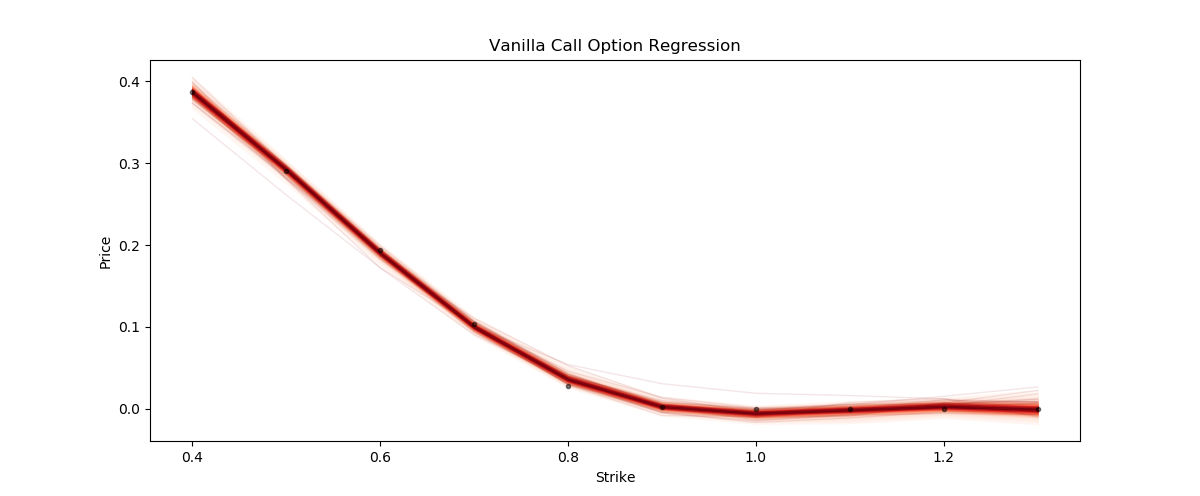
\includegraphics[width=1.1\linewidth]{full_bayesian_1}
     \caption*{Exact GPR: $n= 10$}\label{fig:bayesian_1}
   \end{minipage}\hfill
   \begin{minipage}{0.47\textwidth}
     \centering
     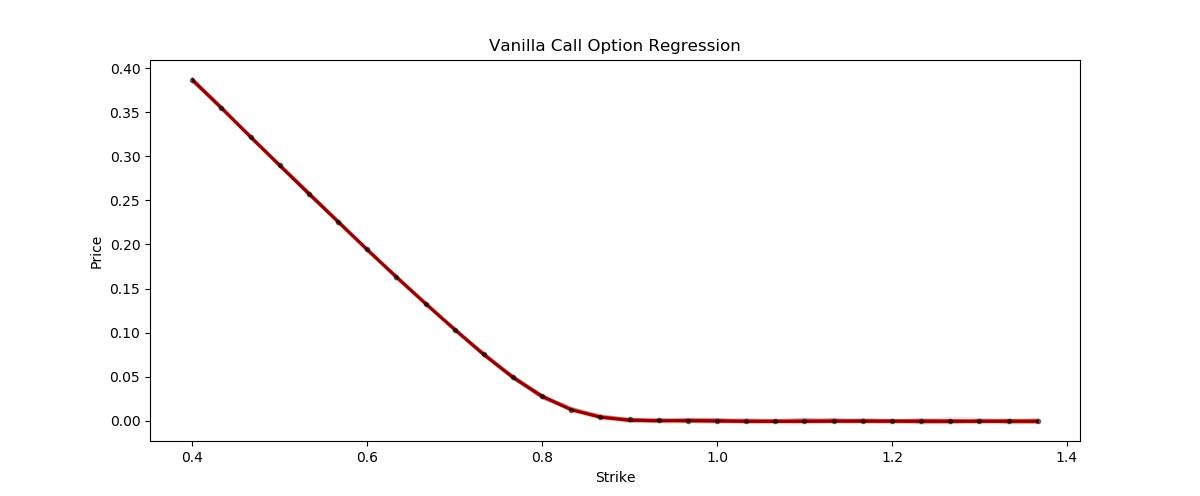
\includegraphics[width=1.1\linewidth]{full_bayesian_2}
     \caption*{Exact GPR: $n=30$}\label{fig:bayesian_2}
   \end{minipage}\hfill
\end{figure}

\begin{figure}[!htb]
   \begin{minipage}{0.47\textwidth}
     \centering
     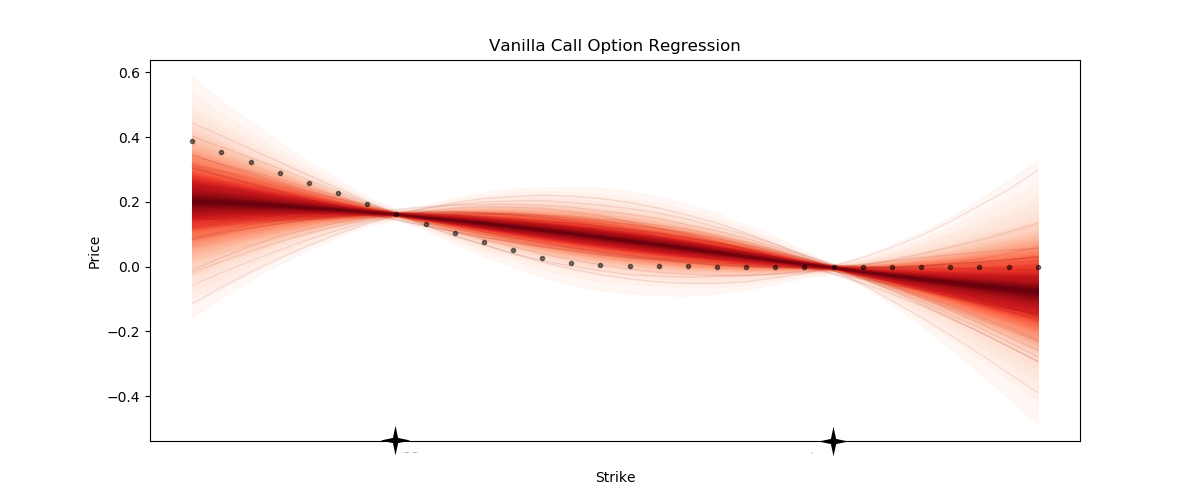
\includegraphics[width=1.1\linewidth]{full_bayesian_3}
     \caption*{FITC: $n=30$, $m=2$}\label{fig:bayesian_3}
   \end{minipage}\hfill
   \begin{minipage}{0.47\textwidth}
     \centering
     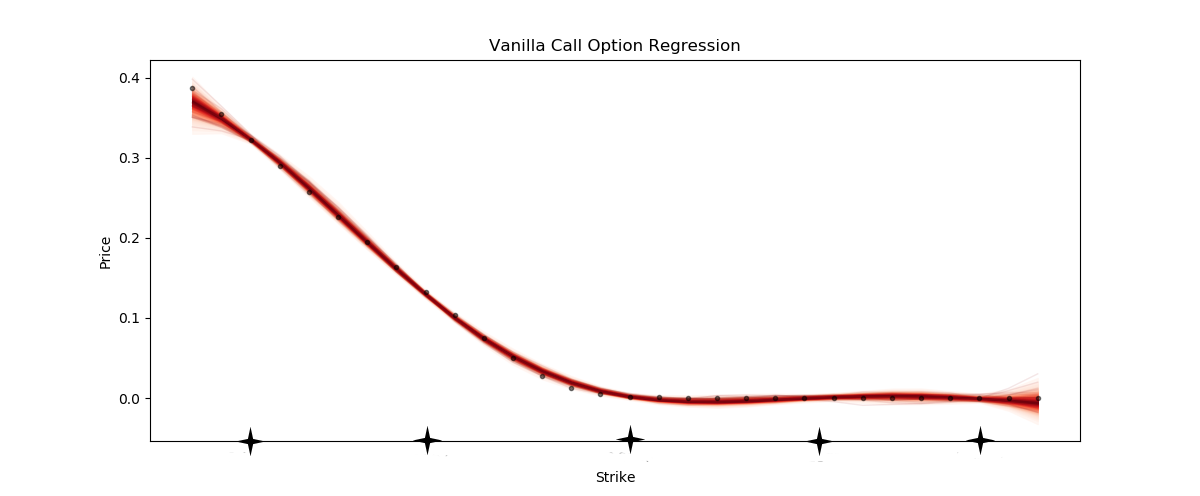
\includegraphics[width=1.1\linewidth]{full_bayesian_4}
     \caption*{FITC: $n=30$, $m=5$}\label{fig:bayesian_4}
   \end{minipage}\hfill
\end{figure}

\begin{figure}[!htb]
   \begin{minipage}{0.47\textwidth}
     \centering
     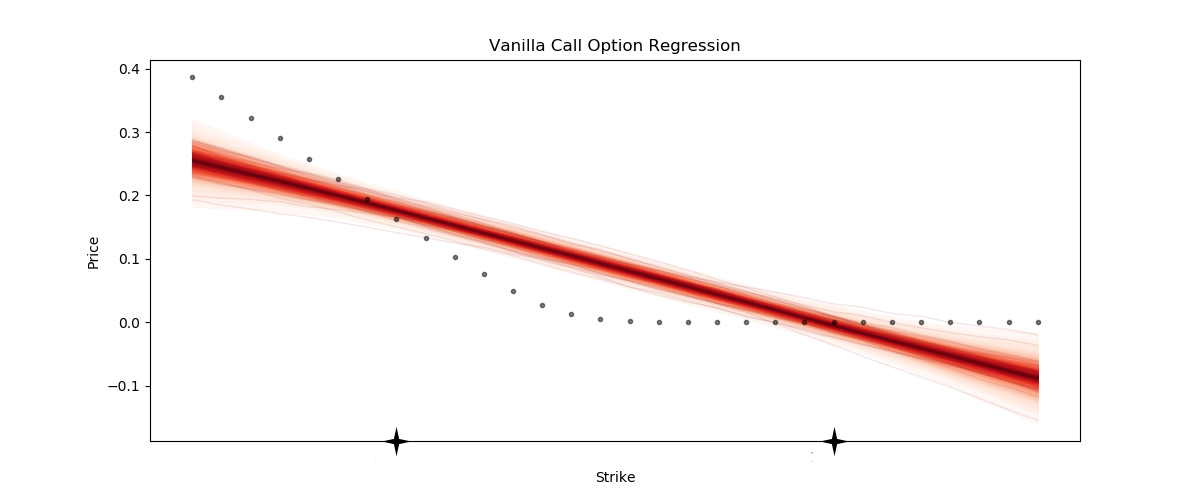
\includegraphics[width=1.1\linewidth]{full_bayesian_5}
     \caption*{VFE: $n=30$, $m=2$}\label{fig:bayesian_5}
   \end{minipage}\hfill
   \begin{minipage}{0.47\textwidth}
     \centering
     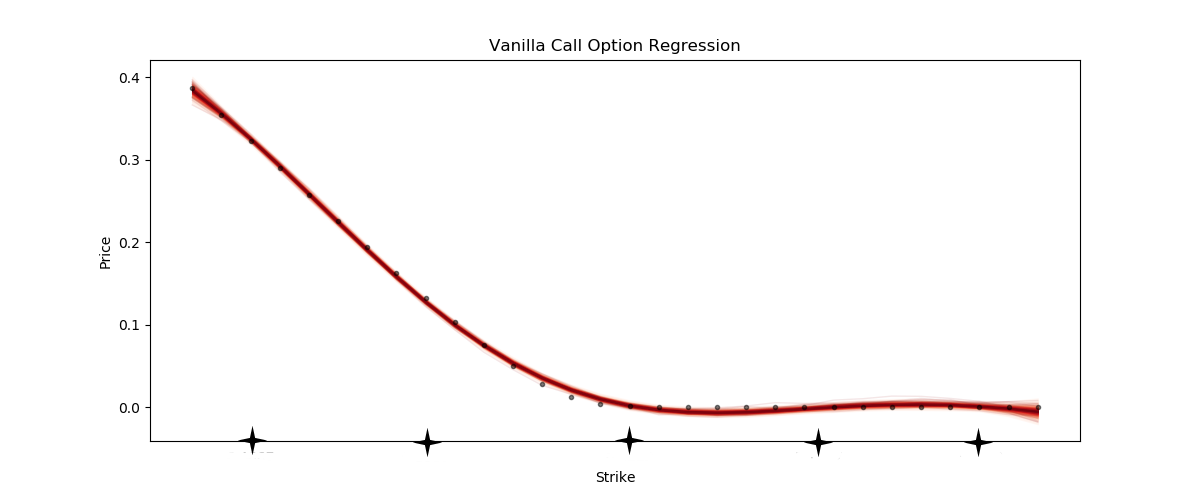
\includegraphics[width=1.1\linewidth]{full_bayesian_6}
     \caption*{VFE: $n=30$, $m=5$}\label{fig:bayesian_6}
   \end{minipage}\hfill
        \caption{Plots price against strike vanilla calls going full bayesian in het Heston model.}\label{fig:bayesian_7}
\end{figure}


\chapter{Scheme and Conclusion}\label{sum_conc}

\section{Scheme}\label{summary}

A handy scheme describing all the models (and their abbreviations) we discussed can be found in figure (\ref{fig:summary}). For BBMM GPR and the Bayesian methods, we only frame the methods we have discussed/referred to using these frameworks although other extensions may be possible like Bayesian polynomial regression. The methods we discussed but which we did not implement in python are in striped cadres.

\newpage

\begin{figure}[!htb]
     \centering
     \includegraphics[width=0.8\linewidth]{scheme_thesis}
     \caption{All the models}\label{fig:summary}
\end{figure}

\section{Conclusion}

The goal of this thesis is fast pricing of derivatives using machine learning techniques. We generated datasets using pricing techniques like FFT, Monte Carlo simulations and binomial trees applied on different financial models which we tried to learn using different GPR models.

The standard algorithm of Gaussian process regression achieves excellent prediction accuracy. However, for large datasets, this methods becomes infeasible to train since it is $O(n^3)$ in computation time. Subsequently, predictions will be relatively slow since they are $O(n)$. Due to the fact that our problems are often high dimensional ($d >5$), standard methods exploiting the structure using Kronecker products and Toeplitz matrices are not suitable. 

Inducing point methods approximate the posterior and we are able to achieve a considerable speed up. For these methods, the time complexity for training is $O(nm^2 + m^3)$ and for predicting $O(m)$. Hence, using few inducing points, fast prediction can be obtained with some loss in accuracy. Since we need to train the locations of the inducing points, slow training and overfitting may occur. Hence, it is recommended to consider k-means for the inducing point locations and to use the VFE method which is protected from overfitting.  

However, we are not yet satisfied due to still punishing train time complexity considering the amount of inducing points. Using stochastic variational GPR, we can use mini batches for training which achieves a huge speed up punishing less the amount of inducing points. Furthermore, we have the same time complexity for prediction as standard inducing methods. 

The methods we have classified under numerical based methods train the models only using matrix vector multiplications (MVMs). Trying to exploit structure (SKI/KISS-GP) for these models, we again stumble on computational issues for high dimensional data. However, using the special properties for product kernels, we can avoid this problem (SKIP) and also obtain a time complexity linear with the amount of data which also does not punish the amount of inducing points in a severe way. Nevertheless,  we encountered stability issues while training for this method since it frequently uses the numerical unstable lanczos decomposition. 

Using approximations the model loses some expressiveness/ predictive ability. Thus we introduced the Blackbox Matrix Matrix (BBMM) framework, enabling straining standard GPR in $O(n^2)$ time and which also achieves considerable speed ups for other methods. Since this framework only uses MVMs, it is possible to enable parallel computations. 


Subsequently, we also discussed Bayesian and deep methods. However, they are more complex and one often needs to sample the predictive posterior which makes prediction slow. 

Finally, we included a data study comparing the models trying to price derivatives and obtaining a considerable speed-up relative to the standard pricing techniques with little loss in accuracy. 












\chapter{Appendix} 

\section{Brownian motion}\label{Brownian_Motion}

We follow \cite{wimschoutensvg}. Let us denote with $\Omega$ the sample space, with $\mathcal{F}$ the event space which is a flow of information i.e. a filtration and with $\mathcal{P}$ the probability function.

\begin{Definition}[Brownian motion]
A stochastic process $X = \{ X_t, t \geq 0 \}$ is a standard Brownian motion on some probability space $(\Omega,\mathcal{F}, \mathcal{P})$, if

\begin{enumerate}
    \item $X_0 = 0$ a.s.
    \item $X$ has independent increments
    \item $X$ has stationary increments
    \item $X_{t+v} - X_t \sim \mathcal{N}(0,v)$.
\end{enumerate}
\end{Definition}


\section{Pricing Derivatives Using Binomial Trees}\label{appendix_tree}

In this section we explain how to use binomial trees to price options. Suppose a stock has initial price $S_0$ and volatility $\sigma$. In our model, there are $2$ possibilities after a small time $\triangle t$. The stock could have gone up having value $S_{\triangle t} = S_0 u= S_0(1+ \sigma \sqrt {\triangle t})$ or down $S_{\triangle t} = S_0 d= S_0(1- \sigma \sqrt{\triangle t})$. Since $\triangle t$ is small, we approximate this using $u = \exp{( 1+ \sigma \sqrt {\triangle t})}$ and $d = \exp{(1- \sigma \sqrt{\triangle t})}$. Denoting with $r$, $q$ the interest and  the dividend rate respectively and assuming a risk neutral world, the probability to go up is equal to

\begin{equation}
p = \dfrac{\exp{((r-q) \triangle t) -d }}{u-d}.
\end{equation}

Hence, the probability to go down is equal to $1-p$. European options can be priced in this way taking the average price of all outcomes of the tree. For American options, it is necessary
to check at each node to see whether early exercise is preferable to holding the option for a further time period $\triangle t$. By working back trough all nodes, we can obtain the value of the option at time zero. By letting $\triangle t \rightarrow 0$, one obtains the Black-Scholes model.  


\section{The FFT Algorithm}\label{Fast_Fourrier_transform}

We now consider how we can evaluate options using the Fast Fourier
Transform (FFT). See \cite{carr1999option} for further details and an improvement for out of the money (OTM) options. Denote with $k$ the log-strike of the strike price $K$. We write with $q_{s_T}(s)$ the risk-neutral density of the log stock price $s_t$ of $S_T$ at maturity $T$ and with $C(K,T)$ be the desired value of a call option with strike $\exp(k)$. We define the characteristic of this density by 

\begin{equation}
\phi_T(u) = \int_{-\infty}^{\infty} e^{ius} q_{s_T}(s) ds.
\end{equation} 

For all the models we discussed (B-S, Heston and VG), a characteristic can be found. We have, including the discounting with expectations
taken under the risk neutral $Q$ measure, that
\begin{align}
C(k,T) &= \exp(-rT) E_Q [ (S_T - k)^+] \nonumber \\
 		&=  \exp(-rT) \int_{k}^{\infty} (e^{s} - e^k) q_{s_T}(s) ds.
\end{align}

However, if $k$ tends to $-\infty$, the call function $C(k, T)$ converges to a non-zero constant (the zero strike call price). Hence, Fourier theory would not apply since this function is not square integrable. In order to obtain a square integrable function, we study the modified call price for some $\alpha > 0$ denoted by 

\begin{equation}
c(k,T) = \exp(\alpha k) C(k,T).
\end{equation} 

Notice that we now need a condition on $\alpha$ for the positive log axis which we discuss later. Next, we take the Fourier transform of $c(k,T)$ and find that 

\begin{align}\label{FFT_1}
\psi(v,T) &= \int_{-\infty}^{\infty} e^{ivk} c(k,T) dk \nonumber  \\
		  &= \int_{-\infty}^{\infty} e^{ivk} \int_{k}^{\infty} e^{\alpha k} e^{-rT} (e^s - e^k) q_{S_T}(s) ds dk \nonumber \\
		  &= \int_{-\infty}^{\infty} e^{-rT} q_{S_T}(s) \int_{-\infty}^{s} (e^{s+\alpha k} - e^{(1+\alpha)k} e^{ivk} dk ds \nonumber \\
		  &= \int_{-\infty}^{\infty} e^{-rT} q_{S_T}(s) \left[\dfrac{e^{(\alpha+1+iv)s}}{\alpha+iv} - \dfrac{e^{(\alpha+1+iv)s}}{\alpha+1+iv}\right] ds \nonumber \\
		  &= \dfrac{e^{-rT} \phi_{T}(v- (\alpha+1)i)}{\alpha^2 + \alpha -v^2 + i(2\alpha+1)v}.
\end{align}

Now, we use the inverse Fourier Transform and find that

\begin{equation}\label{FFT_2}
C(k,T) = \dfrac{e^{-\alpha k}}{2 \pi}\int_{-\infty}^{\infty} e^{-ivk} \psi(v,T) dv = \dfrac{e^{-\alpha k}}{ \pi}\int_{0}^{\infty} e^{-ivk} \psi(v,T) dv.
\end{equation}

Notice for the second equality that $C(K,T)$ is real. This means that $\psi(v,T)$ is even in its real part and odd in its imaginary part. To come back on our problem for (square) integrability for the modified call value in the positive log strike direction, it is satisfactory that $\psi(0,T)$ is finite. Thus, from equation (\ref{FFT_1}) this holds if $\phi_{T}(v- (\alpha+1)i)$ is finite. Hence, an upper bound on $\alpha$ can be found using the characteristic function. Notice that also the last integral of equation (\ref{FFT_2}) can be infinite were another condition concerning $\alpha$ is needed, for which we refer to the original paper. 

Now we are ready to understand how to price options using the FFT. This is an effici\"{e}nt algorithm in order to compute the transform of $\bm{\alpha}_k$ to $\bm{\beta}_k$ with $k \in (1,\ldots,N)$ given by

\begin{equation}\label{FFT_5}
\beta_k = \sum\limits_{j=1}^{N} \exp \left( -\dfrac{2i\pi(j-1)(k-1)}{N}\right)\alpha_j,
\end{equation}

where $N$ is typically a power of $2$.  The algorithm reduces the time complexity from $O(N^2)$ to $O(N \log(N))$. We use the FFT to return $N$ values of $k$ and consider the grid with spacings of size $\lambda$ given by

\begin{equation}\label{FFT_3}
k_u = -\dfrac{N \lambda}{2}  + \lambda(u-1)   \qquad \text{for} \quad u \in (1,\ldots,N).
\end{equation}

This gives us log strike levels ranging from $-\frac{N \lambda}{2}$ until $\frac{N \lambda}{2}$. We use the Simpson's rule (special case of Newton-Cotes formula's) for a good approximation of the integral of equation (\ref{FFT_2}). We denote with $\eta = \frac{v_j}{j-1}$ and with $\delta_{n}$ the Kronecker delta which is zero except for $n =0$ for which it equals one and find that

\begin{equation}\label{FFT_4}
C(k,T) = \dfrac{e^{-\alpha k}}{\pi} \sum\limits^{N}_{j=1} e^{-iv_jk} \psi(v_j,T) \dfrac{\eta(3+(-1)^j-\delta_{j-1})}{3}.
\end{equation}

If we full equation (\ref{FFT_3}) in equation (\ref{FFT_4}) we obtain that 

\begin{equation}\label{FFT_6}
C(k_u,T) = \dfrac{e^{-\alpha k_u}}{\pi} \sum\limits^{N}_{j=1} e^{-iv_j \left( -\frac{N \lambda}{2}  + \lambda(u-1)\right)} \psi(v_j,T) \dfrac{\eta(3+(-1)^j-\delta_{j-1})}{3}.
\end{equation}

In order to apply the FFT, we need that $\lambda \eta = \frac{2\pi}{N}$. We also use that $\eta = \frac{v_j}{j-1}$  and we write $b =\frac{N \lambda}{2} $. We find that 

\begin{equation}
C(k_u,T) = \dfrac{e^{-\alpha k_u}}{\pi} \sum\limits^{N}_{j=1} e^{-i\frac{2\pi}{N}(j-1)(u-1)}e^{ibv_j} \psi(v_j,T) \dfrac{\eta(3+(-1)^j-\delta_{j-1})}{3},
\end{equation}

which has exactly the same form as equation (\ref{FFT_5}) as desired. We will use this equation for pricing vanilla options using the Heston and Variance Gamma model. Of course, appropriate choices for $N$,$\eta$ and $\alpha$ still needs to be chosen. We use $\eta = 0.25$, $N =4096$ and $\alpha = 1.5$ like proposed in the original paper.

\section{Pricing derivatives using Monte Carlo Simulations}\label{derivativesMCS}

In this section, we follow \cite{palczewski2016numerical}. We discuss the Euler and the Milstein scheme and some of its properties. Suppose we have the following stochastic differential equation (SDE) 

\begin{equation}
dX_t = a(X_t) dt + b(X_t) W_t,
\end{equation}

with $a$ and $b$ satisfying some smoothness conditions. We divide a time interval $[0,T]$ into $N$ subintervals with $\delta t = T /N$ and $t_n = n \delta t$. The Euler scheme is given by 

\begin{equation}
X_{t_{n+1}} = X_{t_n} + a(X_{t_n}) \delta t + b(X_{t_n}) (W_{t_{n+1}} - W_{t_n}) .
\end{equation}

Denote with $X_t^{\delta t}$ a process which connects the
points obtained by the numerical scheme with straight lines and with $X_t^{\text{ex}}$ the exact solutions. Denote with $K_T$ a parameter that depends on $T$ and the SDE. A numerical scheme is strongly convergent with order $\gamma$ if

\begin{equation}
\mathbb{E } \left[ |X_t^{\text{ex}} - X_t^{\delta_t}| \right] \leq K_T (\delta_t)^{\gamma}.
\end{equation}



Euler's scheme may not suffice for pricing path-dependent options due to its poor strong convergence to the exact solution. In only converges strongly with order $0.5$, i.e. if we make the step $\delta t$ $100$ times smaller, the approximation only improves with factor $10$.  The Milstein scheme is  obtained as a result of stochastic Taylor expansion or by It\^{o}'s formula and is given by 

\begin{equation}
X_{t_{n+1}} = X_{t_n} + a(X_{t_n}) \delta t + b(X_{t_n}) (W_{t_{n+1}} - W_{t_n}) + \dfrac{1}{2} b' (X_{t_n}) b(X_{t_n}) \left((W_{t_{n+1}} - W_{t_n})^2 - \delta t\right),
\end{equation}

which converges strongly with order $1$. We use this scheme for pricing DOBP options in the Heston model. 


\section{Bayes Theorem}

\begin{Theorem}[Bayes Theorem]
Denote with $A$ and $B$ two random variables. Using the definitions of their conditional probabilities, we obtain Bayes theorem given by
\begin{equation}\label{BayesTheorem}
p(A|B) = \dfrac{p(A)p(B|A)}{p(B)}.
\end{equation}
\end{Theorem}

\section{The Matrix Inversion Lemma}\label{InversionLemma}

In this section we follow \cite{GPRbook}. 

\begin{Lemma}[The Matrix Inversion Lemma]
Denote with $Z$ a $n \times n$ matrix , $W$ a $m \times m$ matrix and $U$ and $V$ are $n \times m$ matrices. Suppose that all necessary inverses exist. The matrix inversion lemma states that 

\begin{equation}
(Z + UWV^t)^{-1} = Z^{-1} - Z^{-1}U(W^{-1} + V^tZ^{-1}U)^{-1} V^tZ^{-1}.
\end{equation}
\end{Lemma}


Notice that if $m <n$, considerable speed-up can be achieved due to inversion of matrices with less dimensions.

\section{Gaussian Identities}\label{Conditioning_of_Gaussians}

In this section, we follow \cite{GPRbook} and \cite{Kuss:06}.

\begin{Lemma} [Linear form of Gaussian] \label{appendix_linearform}
Let $\bm{x} \sim \mathcal{N}(x|\bm{\mu}, \Sigma)$ and $\bm{y} = A \bm{x} + \bm{c}$. We find that $\bm{y} \sim \mathcal{N} (\bm{y}| A \bm{\mu} + \bm{c},  A \Sigma A^t)$.
\end{Lemma}


\begin{Lemma} [Conditional of Gaussians]
Suppose we have that

\begin{equation}
\begin{bmatrix}
    \bm{x}  \\
    \bm{y}
\end{bmatrix}
\sim 
\mathcal{N} \left( \begin{bmatrix}
    \bm{x}  \\
    \bm{y}
\end{bmatrix} \bigg\rvert \begin{bmatrix}
    \bm{\mu_x}  \\
    \bm{\mu_y}
\end{bmatrix}, 
\begin{bmatrix}
    A & \bm{C}\\
    \bm{C}^t  & B
\end{bmatrix} 
\right).
\end{equation} 

Then, supposing that all necessary inverses exist, we find that 

\begin{equation}
\bm{y} | \bm{x} \sim \mathcal{N}(\bm{y} | \bm{\mu_y} + \bm{C}^t A^{-1} (\bm{x} - \bm{\mu_x}), B - \bm{C}^t   A^{-1} \bm{C}).
\end{equation}

\end{Lemma}


\begin{Lemma} [Product of Gaussians]
Let $X \sim \mathcal{N}(\bm{x}|\bm{a},A)$ and $Y \sim \mathcal{N}(\bm{x}|\bm{b},B)$ with $d$ the dimension of $\bm{a}$ and $\bm{b}$. The product of two Gaussians is another (un-normalized) Gaussian given by

\begin{align}
X Y &\sim Z^{-1} \mathcal{N}(\bm{x}|\bm{c},\bm{C}) \\
&  \text{with} \quad \bm{c} = \bm{C}(A^{-1} \bm{a} + B^{-1} \bm{b}) , \quad \bm{C} = (A^{-1} + B^{-1})^{-1} \quad \text{and} \nonumber \\ & Z^{-1} = (2 \pi)^{-d/2} | A + B|^{-1/2} \exp{\left(-\dfrac{1}{2} (\bm{a} - \bm{b} )^t( A +B )^{-1} ( \bm{a} -\bm{b} ) \right)} \nonumber.
\end{align} 
\end{Lemma}

\begin{Lemma}[Gaussian Integrals]\label{appendix_integrals_gaussians} 
The following property holds

\begin{align}
\int_{\mathbb{R}} \mathcal{N}(\bm{x}|\bm{a},A) \mathcal{N}(\bm{a}|\bm{b},B) d\bm{a} = \mathcal{N}(\bm{x}|\bm{b},A +B).
\end{align} 
\end{Lemma}


\section{L-BFGS}\label{appendix_Lbfgs}

In this section, we briefly discuss the L-BFGS methods and follow \cite{liu1989limited}. The BFGS algorithm is a Quasi-Newton method where one approximate the Hessian in each iteration using knowledge of the gradient and the previous approximation of the hessian by a secant condition. L-BFGS is preferable for large datasets since it only uses a limited memory. 


\section{Cholesky decomposition}{\label{Cholesky}

In the section we follow \cite{krishnamoorthy2013matrix}. 

\begin{Definition}[Cholesky Decompostion]
If a matrix $A \in \mathbb{C}$ is a positive definite Hermitian matrix, the Cholesky decompostion factorises the matrix into a product of a lower triangular matrix $L$ and its conjugate transpose $L^{\ast}$ i.e. 
\begin{equation}
A = L L^{\ast}
\end{equation}
\end{Definition}

This factorisation is of order $O(n^3)$. We only use real matrices and we work from now with $L^{\ast} = L^t$. Inversion based on Cholesky decomposition is numerically stable for well conditioned matrices. The inverse can be found using 

\begin{equation}
(L L^{t})^{-1} = (L^t)^{-1} L^{-1}.
\end{equation}

The inverse of triangular matrices can be calculated in a recursive fashion. Remember that the determinant of the product equals the product of the determinants and that the determinant of a triangular matrix equals the sum of its trace. Hence, the determinant of $A$ equals the determinant of $L$ multiplied with the determinant of $L^t$ which equals the square of the sum of the diagonal elements of $L$. 

\section{The Kronecker product}\label{Kronecker_product}

We state the most important properties of the Kronecker product found in \cite{saatcci2012scalable} where one can find the corresponding proofs. 

\begin{Definition}[Kronecker product]\label{Kronecker_definition}
Let $A$ be a $m \times n$ matrix and $B$ a $p \times q$ matrix. The Kronecker product of these two matrices is given by 
\begin{equation}
A \otimes B
= \begin{bmatrix}
    a_{11}B & \cdots & a_{1n}B  \\
    \vdots    &    \ddots          &  \vdots   \\
    a_{m1}B & \cdots & a_{mn}B
\end{bmatrix}, 
\end{equation} 
which is a $ mp \times nq$ matrix. Let us denote with $A_c$ an $e_c \times e_c$ matrix and with $N = \prod_{c=0}^d e_c$. Using Kronecker products, we say that matrix indices start at zero for simplicity. We impose that 
\begin{enumerate}
\item $0 \leq i^{(c)},j^{(c)} < e_c$ (matrix indices start at zero),
\item $0\leq i < N$ and $ 0\leq j < N$
\item  $i= \sum\nolimits_{c=1}^d (e_c)^c i^{(c)}$ and $ j= \sum\nolimits_{c=1}^d (e_c)^c j^{(c)}$.
\end{enumerate}
Hence, we find for the more general equation $A = A_1 \otimes \cdots \otimes  A_d = \bigotimes_{c=1}^d A_c$ that

\begin{equation}\label{Kronecker1}
A(i,j) = A_1(i^{(1)},j^{(1)})A_2(i^{(2)},j^{(2)}) \cdots A_d(i^{(d)},j^{(d)}). 
\end{equation}
\end{Definition}


Next, we list some important properties of the Kronecker product. 
\begin{Properties}[Kronecker product]\label{Properties_Kronecker}
Denote with $A$ and $B$ two square matrices with dimension $N_a$ and $N_b$ respectively. We have that 
\begin{itemize}
\item $\det(A \otimes B) = \det(A)^{N_a}  \det(B)^{N_b}$
\end{itemize}
Subsequently, suppose that $K = \bigotimes_{c=1}^d K_c$, we have that 
\begin{itemize}[resume]
\item $K^{-1} = \bigotimes\limits_{c=1}^d K_c^{-1}$
\end{itemize}
Furthermore, if $K = \bigotimes_{c=1}^d K_c$ and $K = L L^t$ and $K_c = L_c L_c^t$, we find that
\begin{itemize}[resume]
\item $L = \bigotimes\limits_{c=1}^d L_c$
\end{itemize}
A very similar result can be obtained for the eigendecompositions. If $K = \bigotimes_{c=1}^d K_c$ and let $K_c = Q_c \Lambda_c Q_c^t$ the eigendecomposition of $K_c$. Then the eigendecomposition for $K = Q \Lambda Q^t$ has the following properties
\begin{itemize}[resume]
\item $Q = \bigotimes\limits_{c=1}^d Q_c$
\item $\Lambda = \bigotimes\limits_{c=1}^d \Lambda_c$
\end{itemize}

\end{Properties}

\section{K-means} \label{appendix_kmeans}

In this section, we follow \cite{pptkmeans}. We discuss the K-means algorithm in its most basic form (LLoyd's method) and give some possible extensions. First, choose the amount of data clusters we want to obtain. In our case, this is the amount of inducing points $m$. From now, we denote with $\bm{c}_1, \ldots, \bm{c}_m $ the cluster centres and with $C_1, \ldots, C_m $ the clusters. However, we have to initialise the center of our clusters. These points can be chosen at random which is not recommended since one probably initialises multiple points in one cluster. Hence, using a heuristic is recommended. A popular heuristic is the furthest point heuristic where one picks centres among the data points furthest away from the previously chosen centres. Notice that this method performs poorly if there are a lot of outliers. A very popular algorithm for choosing the initial values is the k-means++ initialisation (see algorithm (\ref{k-means++ initialisation})), which spreads out the initial cluster centers. 

\begin{algorithm}
\caption{k-means++ initialisation}\label{k-means++ initialisation}
\begin{algorithmic}[1]
\item \textbf{input}: $X$
\item  \textbf{output}: $\bm{c}_1, \ldots, \bm{c}_m $ 
\BState
\BState Pick \emph{$\bm{c}_1$} arbitrary
\BState For \emph{$j = 2, \ldots, m$} do:
\State \quad Pick \emph{$\bm{c}_j$} among \emph{$(\bm{x}_1, \ldots, \bm{x}_n)$} according to distribution \emph{$ P(\bm{c}_j = \bm{x}_i) \propto \min\limits_{j' < j} ||\bm{x}_i - \bm{c}_{j'} || ^2$}.
\end{algorithmic}
\end{algorithm}


The time complexity of the k-means++ initialisation is $O(n m d)$. Now LLoyd's algorithm with $p$ iterations is given in algorithm (\ref{LLoyd's algorithm}).

\begin{algorithm}
\caption{LLoyd's algorithm}\label{LLoyd's algorithm}
\begin{algorithmic}[1]
\item \textbf{input}: $X$ and $\bm{c}_1, \ldots, \bm{c}_m $ (initial cluster centers) 
\item  \textbf{output}: $\bm{c}_1, \ldots, \bm{c}_m $ (updated cluster centers) and $\bm{C}_1, \ldots, \bm{C}_m $ (the clusters)
\BState
\BState For \emph{$i = 1, \ldots, p$} do:
\BState \quad For \emph{$i = 1, \ldots, n$} do:
\State \quad \quad \emph{$\bm{x}_i \in C_j$} if \emph{$\bm{x}_i $} closed to \emph{$\bm{c}_j$} with \emph{$j \in ( 1, \ldots, m)$}
\BState \quad For \emph{$j = 1, \ldots, m$} do:
\State \quad \quad Set \emph{$\bm{c}_j$} mean of values in $C_j$
\end{algorithmic}
\end{algorithm}

One can choose a metric to calculate the distances between the points. By running a fixed number of $p$ iterations (or using an upper bound of $p$ iterations), the time complexity of this algorithm is given by $O(n m d p)$.  Hence the accumulation of LLoyd's algorithm with k-means++ initialisation is $O(n m d p)$. For large problems, one can use mini-batches to update centre positions.  

\section{Sylvester's Determinant Identity}\label{Sylvester}

We state the theorem found in \cite{ambikasaran2014fast}.

\begin{Lemma}[Sylvester's Determinant Identity]
If $A \in \mathbb{R}^{m \times n}$ and $B \in \mathbb{R}^{n \times m}$, we find that

\begin{equation}
\det{(I_m + A B)} = \det{(I_n + B A)}.
\end{equation} 

\end{Lemma} 

\section{The Kullback-Leibler (KL) divergence and Variational Lower bound} \label{KL}

In this section, we follow \cite{blei2017variational} and \cite{yang2017understanding}. We denote with $\bm{y}$ the observations and $\bm{z}$ the latent variables. 

\begin{Definition}[Kullback-Leibler (KL) divergence and Variational Lower bound]
The Kullback-Leibler (KL) divergence is a measure of the closeness of two distributions, which we denote with $q(\bm{z})$ and $p(\bm{z}|\bm{y})$, given by
\begin{align}
\text{KL}(q(\bm{z})||p(\bm{z}|\bm{y})) &:= \mathbb{E}_q \left[ \log \dfrac{q(\bm{z})}{p(\bm{z}|\bm{y})} \right]
\nonumber \\ &= \mathbb{E}_q[\log{q(\bm{z}})] - \mathbb{E}_q[\log{p(\bm{z}})|\bm{y}] \nonumber \\
&= \mathbb{E}_q[\log{q(\bm{z}})] - \mathbb{E}_q[\log{p(\bm{z}},\bm{y})] + \log{p(\bm{y})} \nonumber \\
&= -\mathcal{L}(q) + \log{p(\bm{y}}).
\end{align}
The Variational Lower bound (often called evidence lower bound (ELBO) is by definition equal to $\mathcal{L}(q)$. 
\end{Definition}

Now, one can find the following important theorem. 

\begin{Theorem}
$\mathcal{L}(q)$ is a lower bound for $\log{p(\bm{y}})$ .
\end{Theorem}

\begin{proof}
It is sufficient to prove that the KL divergence of two distributions is always positive, from which the desired property holds. The proof is nothing more than Jensen's inequality for concave functions. Jensen's inequality states that for a concave function $h$ and a r.v. $X$

\begin{equation}
 \mathbb{E} [h(X)] \overset{\mathrm{J.}}{\leq} h(\mathbb{E}[X]).
\end{equation}

For convex functions, the opposite holds. Noting that the logarithm is a concave function and the expectation a linear operator, we find that

\begin{align}
-\text{KL}(q(\bm{z})||p(\bm{z}|\bm{y})) &= \mathbb{E}_q \left[ -\log \left( \dfrac{q(\bm{z})}{p(\bm{z}|\bm{y})} \right) \right]
\nonumber \\ &= \mathbb{E}_q \left[ \log \left( \dfrac{p(\bm{z}|\bm{y})}{q(\bm{z})} \right) \right]
\nonumber \\ &\overset{\mathrm{J.}}{\leq}  \log \left( \mathbb{E}_q \left[  \dfrac{p(\bm{z}|\bm{y})}{q(\bm{z})} \right] \right) \nonumber \\
&= \log(1) = 0  
\end{align} 
\end{proof}

We state an exact expression for the KL-divergence between two multivariate Gaussians found in \cite{duchi2007derivations}

\begin{Lemma}\label{KL_gaussian}
Suppose that $q \sim \mathcal{N}(\bm{z}|\bm{\mu}_1, \Sigma_1)$ and $p \sim \mathcal{N}(\bm{z}|\bm{\mu}_2, \Sigma_2)$. We find that 

\begin{equation}
\text{KL} (q(\bm{z})||p(\bm{z})) = \dfrac{1}{2} \left( \log \left( \dfrac{|\Sigma_2|}{|\Sigma_1|} \right) - d + \Tr ( \Sigma_2^{-1} \Sigma_1) + (\bm{\mu}_2 - \bm{\mu}_1)^t \Sigma_2^{-1} (\bm{\mu}_2 - \bm{\mu}_1) \right).
\end{equation}
\end{Lemma}


\section{Stochastic Variational Inference and Stochastic Gradient methods} \label{appendix_var_inf}

 
In this section, we follow \cite{bottou2010large} and \cite{blei2017variational}. We use the same notation as in the previous section. We need that the variational objective (f.e. the ELBO) decomposes into a sum of terms, one for each data point in the analysis, so we can use stochastic optimisation. In order to do so, we strive for a structure like in figure (\ref{fig:var_app_1.1}). The distribution of each observation $y_i$ only corresponds on its latent/local variable $z_i$ and the global variables $\bm{g}$. 

\begin{figure}[!htb]
     \centering
     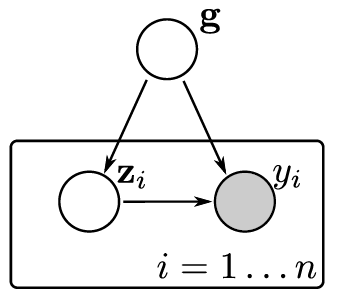
\includegraphics[width=0.4\linewidth]{plot_variational_inference}
     \caption{Figure from \cite{hensman2013}. Requirements for SVI}\label{fig:var_app_1.1}
\end{figure}

Let us denote with $\bm{\theta}$ the family of parameters we want to optimize by minimising the loss $\mathcal{L}(\bm{z},\bm{y},\bm{\theta})$. Suppose that this loss can be decomposed in a sum such that 

\begin{equation}
\mathcal{L}(\bm{z},\bm{y},\bm{\theta}) = \sum\limits_{i=1}^n l (z_i,y_i,\bm{\theta})
\end{equation}

Using the ordinary gradient descent, we can update the parameters by taking steps (with a gain/learning rate $\gamma$) in the direction of the gradient. Notice also the strong similarities with the famous Newton-based optimisation algorithms and remember that the gradient is the direction of the steepest ascent. We find that 

\begin{equation}\label{gradient_descent}
\bm{\theta}_{t+1} = \bm{\theta}_{t} -  \gamma \dfrac{1}{n} \sum\limits_{i=1}^n \bigtriangledown l(z_i,y_i,\bm{\theta})
\end{equation}

One can achieve linear convergence when, under sufficient regularity conditions, the initial value $\theta_0$ is close enough to the optimum and the gain is sufficiently small. A second order gradient descent can be found by by replacing the scalar gain $\gamma$ by a positive definite matrix that approaches the inverse of the Hessian of the cost at the optimum. Now, stochastic gradient descent calculates the gradient of one arbitrary point (of a batch $B$ containing arbitrary points with a specified size) and one does


\begin{equation}\label{stoch_gradient_descent}
\bm{\theta}_{t+1} = \bm{\theta}_{t} -  \gamma_t \dfrac{1}{n} \sum\limits_{b \in B } \bigtriangledown l(z_b,y_b,\bm{\theta}).
\end{equation}

This is of course less computationally demanding and results often only in a slightly lower convergence rate. Convergence results usually require decreasing gains satisfying the conditions $\sum\nolimits_t \gamma_t^2 < \infty$ and $\sum\nolimits_t \gamma_t = \infty$ and some mild conditions. The best convergence speed is achieved using gains $\gamma_t \sim t^{-1}$. This method works when equation (\ref{stoch_gradient_descent}) behaves like its expectation equation (\ref{gradient_descent}) despite the noise introduced by this simplified procedure. However, a bad choice of the learning rate can be problematic. Hence, a more advanced optimise, for example the Adam optimiser (see section \ref{appendix_adam}), is recommended. 

\section{Adam Optimiser}\label{appendix_adam}

In this section, we follow \cite{kingma2014adam}. Adam only requires first-order gradients for efficient stochastic optimization with little memory requirement. Using estimates for the first and second moment of the gradient, the method computes individual adaptive learning rates. The algorithm and more information can be found in the source.

\section{The Natural Gradient}\label{appendix_nat_grad}


In this section, we give a short outline about gradients and follow \cite{hoffman2013stochastic}. For the classical gradient method, one can optimise a function $f(\bm{\lambda})$ by taking steps (with a step-size) in the direction of the gradient. Remember that the gradient is the direction of the steepest ascent. Thus the direction of the gradient $\bigtriangledown_{\bm{\lambda}} f(\bm{\lambda})$ points in the same direction as the solution of the problem 

\begin{equation}
\text{arg max}_{d\bm{\lambda}} (f(\bm{\lambda) + d\bm{\lambda}})  \qquad \text{subject to} \quad ||d\bm{\lambda}||^2 < \varepsilon,
\end{equation}

for sufficient small $\varepsilon$. Notice that the direction of the gradient depends on the Euclidian distance metric which is often a poor measure of the dissimilarity of distributions $p(g|\lambda)$ and $p(g|\lambda'$. For example, suppose that $p(g)$ is the univariate normal with the parameter $\bm{\lambda})$ equal to the mean $\mu$ and standard deviation $\sigma$. The distributions $\mathcal{N}(0,10000)$ and $\mathcal{N}(10,10000)$ are almost indistinguishable and the Euclidean distance equals $10$. However, the distributions $\mathcal{N}(0,0.01)$ and $\mathcal{N}(0.1,0.01)$ barely overlap and their Euclidean distance equals $0.01$. 

Hence, we need the introduce the concept of natural gradient. This is based on the symmetrized KL divergence given by

\begin{equation}
D_{KL}^{sym}(\bm{\lambda}, \bm{\lambda'}) = \mathbb{E}_{\bm{\lambda}}\left[\log{\dfrac{p(g|\bm{\lambda)}}{p(g|\bm{\lambda')}}}\right] + \mathbb{E}_{\bm{\lambda'}}\left[\log{\dfrac{p(g|\bm{\lambda')}}{p(g|\bm{\lambda)} }}\right]
\end{equation}


The natural gradient $\hat{\bigtriangledown}_{\bm{\lambda}} f(\bm{\lambda})$points in the same direction as the solution of the problem 

\begin{equation}
\text{arg max}_{d\bm{\lambda}} f(\bm{\lambda) + d\bm{\lambda}})  \qquad \text{subject to} \quad D_{KL}^{sym}(\bm{\lambda}, \bm{\lambda} + d\bm{\lambda})  < \varepsilon,
\end{equation}

with $\varepsilon$ small enough. Denoting with $I(\bm{\lambda})$ the fisher information matrix of $p(\bm{\lambda})$, one has shown that the natural gradient equals 

\begin{equation}
\hat{\bigtriangledown}_{\bm{\lambda}} f(\bm{\lambda}) = I(\bm{\lambda})^{-1} \bigtriangledown_{\bm{\lambda}} f(\bm{\lambda})
\end{equation}

We will not go in detail about exponential families. However, the natural gradient is easily computable in this case (even easier as the normal gradient).  

\section{A Short Notion About Interpolation}\label{appendix_interpolation}

In the first part of this section, we follow \cite{keys1981cubic}. 

In order to have clear notation, we only describe the 2-dimensional case. Denote with $h_x$ and $h_y$ the sample increments, $(x_k,y_l)$ the interpolation nodes, $u$ the interpolation kernel and $f$ the sampled function. For equally spaced (in each dimension) data, any interpolation function (2D) can be written in the form 

\begin{equation}\label{general_form}
g(x,y) = \sum_{k} \sum_l c_{k,l} u \left( \dfrac{x - x_k}{h_x} \right)  u \left( \dfrac{y - y_l}{h_y} \right),
\end{equation}

since we assume that $u(0) = 1$. Since we interpolate $f$, we want $g(x_k,y_l) = f(x_k,y_l)$. Hence, we replace all the $c_{k,l}$ by the sampled data i.e. $c_{k,l} = f(x_k,y_l)$. The linear interpolation kernel is given by 

 \begin{equation}
    u(s)=
    \begin{cases}
      -s+1, & \text{if}\ 0 < s < 1 \\
      s+1, & \text{if}\ -1 < s \leq 0 \\
      0 & \text{if}\ |s| \geq 1 .
    \end{cases}
 \end{equation}
 
The cubic convolution interpolation kernel is given by 

\begin{equation}
    u(s)=
    \begin{cases}
      \dfrac{3}{2}|s|^3 - \dfrac{5}{2}|s|^2 +1 & \text{if}\ 0 \leq |s| < 1 \\
      -\dfrac{1}{2} |s|^3 + \dfrac{5}{2}|s|^2 - 4|s| +2, & \text{if}\ 1 \leq |s| < 2 \\
      0 & \text{if}\ |s| \geq 2 .
    \end{cases}.
\end{equation}

In this case, the interpolation error goes to zero
uniformly at a rate proportional to $O(h^3)$. However, equispaced grids are not always applicable. In this case, one can use local inverse distance weighting interpolation, which can be applied to irregular grids. From now, we follow \cite{babak2009statistical}.  It is defined as a spatially weighted average of the sample values within a search neighbourhood $U_x$. Suppose $d$ is the Euclidian metric, although other possibilities are possible.

Let us denote 

\begin{equation}
\lambda_i(\bm{x}) = \dfrac{\frac{1}{d(\bm{x}_i,\bm{x})}}{\sum\limits_{j : \bm{x}_j \in U_{\bm{x}}} \frac{1}{d(\bm{x}_j,\bm{x})}}.
\end{equation}

Then local inverse distance weighting interpolation is calculated as 

\begin{equation}
g(\bm{x}) = \sum\limits_{i : \bm{x}_i \in U_{\bm{x}}}  \lambda_i(\bm{x}) f(\bm{x}_i).
\end{equation}


\section{The Lanczos decomposition}\label{appendix_lanczos_dec}


In this section, we follow \cite{gardner2018gpytorch} and chapter $10$ of \cite{arbenz2012lecture} which is clearly written. The Lanczos decomposition executes an orthogonal transformation from a Hermitian matrix to a tridiagonal form. It is a simplification of the Arnoldi algorithm using the Hermitian property.  Let $A$ be a $n \times n$ an Hermitian matrix and $\bm{x}$ a generating vector. The Lanczos decomposition computes an orthonormal basis of the Krylov space $\mathcal{K}^j(\bm{x}, A) = \text{span} \{ \bm{x},A \bm{x}, \ldots, A^{j-1} \bm{x} \}$. As one could suspect, one uses the Gram–Schmidt orthogonalization process and exploits the hermitian form. Now, let $Q_k$ be a $n \times k$ matrix representing the orthonormal basis for $\mathcal{K}^{k}(\bm{x}, A)$ and $T_k$ a tridiagonal $k \times k$ matrix. The Lanczos relation is given by

\begin{equation}
A Q_k = Q_k 
	\underbrace{\begin{bmatrix}
    \alpha_1 & \beta_1& & & \\
    \beta_1  &\alpha_2 & \beta_2 & &\\
     & \beta_2 & \alpha_3 & \ddots &  \\
     & & \ddots   &\ddots & \beta_{k-1} \\
     & & & \beta_{k-1} & \alpha_k 
	\end{bmatrix}}_{T_k}  + \beta_k [\underbrace{\bm{0}, \ldots, \bm{0}}_{k-1}, \bm{q}_{k+1}]^t.
\end{equation}

Remember that the inverse of an orthogonal matrix equals the transpose. Hence, this procedure yields a low-rank approximate tridiagonalisation 

\begin{equation}
A \approx Q_k T_k Q_k^t.
\end{equation}

Now let $m$ be the smallest index such that $\mathcal{K}^{m}{\bm{x}} = \mathcal{K}^{m+1}{\bm{x}}$. Notice also that the set $\{1, A, A^2, \ldots , A^n \}$ is linearly dependent for any matrix $A$. Hence, for $n$ iterations this procedure produces always an exact iteration. Then $\beta_k =0$ and we obtain 

\begin{equation}
A Q_m = Q_m T_m
\end{equation}

with $Q_m = [\bm{q}_1, \ldots, \bm{q}_m]$ ($\bm{q}_1$ is $\bm{x}$) and we find $A = Q_m T_m Q_m^t$. The algorithm can be found in \cite{arbenz2012lecture}.  The main results are that in a single iteration step, we only have to execute a matrix-vector multiplication, $7n$ further floating point operations and that the eigenvalues of $T_m$ equals the eigenvalues of $A$. However, the Lanczos tridiagonalization algorithm has storage and numerical stability issues. 


\section{Conjugate Gradient Method} \label{appendix_conj_grad}

In the previous sections of the appendix about numerical techniques (Cholesky decomposition, L-BFGS, Adam, Lanczos decomposition, ...) we omitted the pseudo-code and its derivations which can be found in the corresponding sources. However, this algorithm will be modified and used to retain the Lanczos tridiagonal matrix $T$, thus a more expanded discussion is appropriate. Nevertheless, one can also directly go to algorithm (\ref{c_g_algorithm}). First, we follow \cite{shewchuk1994introduction} where the derivations can be found and which is a piece of art. The conjugate gradient (CG) tries to find the solution of a numerical system of linear equations and is faster than the steepest decent (due to zigzagging etc.). The quadratic form 

\begin{equation}\label{quad_eq}
f(\bm{x}) = \dfrac{1}{2} \bm{x}^t A \bm{x} - \bm{b}^t \bm{x} + c
\end{equation}

is minimised by the solution of $A \bm{x} = b$ if $A$ is symmetric. Hence, we can try to find a method minimising equation (\ref{quad_eq}). We denote with $\bm{e}_{(i)} = \bm{x}_{(i)} - \bm{x}$ the error, with $\bm{r}_{(i)} = \bm{b} - A\bm{x}_i$ the residual and with $\bm{d}_{(i)}$ the search directions. It is easy to see that $\bm{r}_{(i)} = - A \bm{e}_{(i)}$. Notice that $\bm{r}_{(i)} = -f(\bm{x}_{(i)})$, which implies that the residual is the direction of steepest descent. For each step we choose a point

\begin{equation}
\bm{x}_{(i+1)} = \bm{x}_{(i)} + \alpha_{(i)} \bm{d}_{(i)}.
\end{equation}

The main question is, how big must the step $\alpha$ be?
Two vectors $\bm{d}_{(i)}$ and $\bm{d}_{(j)}$ are A-orthogonal or conjugate if $ \bm{d}_{(i)}^t A \bm{d}_{(j)} = 0$. We require that $\bm{e}_{(i+1)}$ is A-orthogonal to $\bm{d}_{(i)}$. This is equivalent to finding the minimum point along the search direction since

\begin{equation}
\dfrac{d}{d \alpha} f(\bm{x}_{(i+1)})  = 0 \Leftrightarrow f'(\bm{x}_{(i+1)})^t  \dfrac{d}{d \alpha} \bm{x}_{(i+1)}= 0 \Leftrightarrow - (\bm{r}_{(i+1)})^t \bm{d}_{(i)} = 0  \Leftrightarrow \bm{d}_{(i)}^t A \bm{e}_{(i+1)} = 0.
\end{equation}

This implies that 

\begin{equation} \label{search_direction}
\bm{d}_{(i)}^t A \bm{e}_{(i+1)} =0 \Leftrightarrow \bm{d}_{(i)}^t A (\bm{e}_{(i)} + \alpha_{(i)} \bm{d}_{(i)}) = 0 \Leftrightarrow \alpha_{(i)} = \dfrac{\bm{d}_{(i)} \bm{r}_{(i)} }{ \bm{d}_{(i)}^t A \bm{d}_{(i)}}. 
\end{equation}

Now we try to find A-orthogonal search directions. We generate them using the conjugate Gram-Schmidt process. Suppose we have a set $\bm{u}_0, \ldots, \bm{u}_{n-1}$, which are linearly independent vectors. Set $\bm{d}_{0} = \bm{u}_0$ and for $i>0$ set 

\begin{equation}\label{gram-schmidt}
\bm{d}_{(i)} = \bm{u}_i + \sum\limits_{k=0}^{i-1}\beta_{ik} \bm{d}_{(k)}
\end{equation}

with 

\begin{equation}
\beta_{(i,j)} = - \dfrac{\bm{u}_{i}^t A \bm{d}_{(j)}}{\bm{d}_{(j)}^t A \bm{d}_{(j)}}.
\end{equation}

Hence, we subtract out any components that are not A-orthogonal to the previous $\bm{d}$ vectors. By taking the product of equation (\ref{gram-schmidt}) with $\bm{r}_{(i)}$, one finds that 

\begin{equation} \label{conjugate_grad_3}
\bm{d}_{(i)}^t \bm{r}_{(i)} = \bm{u}_{(i)}^t \bm{r}_{(i)}.
\end{equation}


Now, the error term is A-orthogonal to all old search directions. Because  $\bm{r}_{(i)} = - A \bm{e}_{(i)}$ each residual is orthogonal to the previous search directions. This also implies that each residual is  orthogonal to the previous residuals. Now seeing that 

\begin{equation}\label{Conj_grad_1}
\bm{r}_{(i+1)} = -A \bm{e}_{(i+1)} = -A (\bm{e}_{(i)} + \alpha_{(i)} \bm{d}_{(i)}) = \bm{r}_{(i)}  - \alpha_{(i)} A \bm{d}_{(i)},
\end{equation}

we find that each residual is linear combination of $A \bm{d}_{(i)}$ and the previous residual. Hence, the linear space of residuals $\text{span} \{ \bm{r}_{(0)}, \ldots, \bm{r}_{(i)} \}$ equals the Krylov space $
\mathcal{K} (\bm{r}_{(0)}, A)$. Now, the Gram-Schmidt constants are given by

\begin{equation} \label{Gram_schmidt_2}
\beta_{(i,j)} = -\dfrac{\bm{r}_{(j)} A \bm{d}_{(j)}}{\bm{d}_{(j)} A \bm{d}_{(j)} }.
\end{equation}

Taking the inner product from equation (\ref{Conj_grad_1}), we find that 

\begin{align}
\bm{r}_{(i)}^t \bm{r}_{(j+1)} &= \bm{r}_{(i)}^t \bm{r}_{(j)} - \alpha_{(j)} \bm{r}_{(i)}^t A \bm{d}_{(j)} \nonumber \\
\alpha_{(j)} \bm{r}_{(i)}^t A \bm{d}_{(j)} &= \bm{r}_{(i)}^t \bm{r}_{(j)} - \bm{r}_{(i)}^t \bm{r}_{(j+1)} .
\end{align}

Now, since each residual is  orthogonal to the previous residuals, we find that

\begin{equation}
 \bm{r}_{(i)}^t A \bm{d}_{(j)}  = \left\{
  \begin{array}{@{}ll@{}}
    \frac{1}{\alpha_{(i)}} \bm{r}_{(i)}^t  \bm{r}_{(i)}   & \text{if}\ i = j \\
     \frac{1}{\alpha_{(i-1)}} \bm{r}_{(i)}^t  \bm{r}_{(i)} &\text{if}\ i = j+1 \\ 
     0 &  \text{otherwise}.
  \end{array}\right.
\end{equation}

Hence, we find that 

\begin{equation}
\beta_{(i,j)} = \left\{
  \begin{array}{@{}ll@{}}
    \frac{1}{\alpha_{(i-1)}} \dfrac{\bm{r}_{(i)}^t  \bm{r}_{(i)}}{\bm{d}^t_{(i-1)} A \bm{d}_{(i-1)} }  & \text{if}\ i = j+1 \\
     0 &  \text{if}\ i > j+1,
  \end{array}\right.
\end{equation}

which means that most of the  $\beta_{(i,j)} $ terms disappear making the calculations much faster. Now using the abbreviation $\beta_{(i)} = \beta_{(i,i+1)}$ and equation (\ref{search_direction}}), (\ref{conjugate_grad_3}), we find that 

\begin{align}
\beta_{(i)} &= \dfrac{\bm{r}_{(i)}^t  \bm{r}_{(i)}}{\bm{d}^t_{(i-1)} \bm{r}_{i-1}}  \nonumber \\
&= \dfrac{\bm{r}_{(i)}^t  \bm{r}_{(i)}}{\bm{r}_{(i-1)}^t  \bm{r}_{(i-1)}}.
\end{align}

Putting everything together, we find algorithm (\ref{c_g_algorithm}).


\begin{algorithm}
\caption{Conjugate Gradient Method}\label{c_g_algorithm}
\begin{algorithmic}[1]
\item \textbf{input}: $A, \bm{b}$
\item \textbf{output}: $A^{-1} \bm{b}$
\BState \emph{ $\bm{x}_{(0)} = 0$}
\BState Compute \emph{$\bm{d}_{(0)} = \bm{r}_{(0)} = \bm{b} - A \bm{x}_{(0)}$}
\BState For \emph{$i = 0, \ldots, p$} do :
\State \quad $\alpha_{(i)} = \dfrac{\bm{d}_{(i)}^t \bm{r}_{(i)} }{ \bm{d}_{(i)}^t A \bm{d}_{(i)}}$
\State \quad $\bm{x}_{(i+1)} = \bm{x}_{(i)} + \alpha_{(i)} \bm{d}_{(i)}$
\State \quad $\bm{r}_{(i+1)} = \bm{r}_{(i)}  - \alpha_{(i)} A \bm{d}_{(i)}$
\State \quad If \emph{$||\bm{r}_{(i+1)}||_2 < \text{tolerance}$}, then return \emph{$\bm{x}_{(i+1)}$}
\State \quad $\beta_{(i)} = \dfrac{\bm{r}_{(i+1)}^t  \bm{r}_{(i+1)}}{\bm{r}_{(i)}^t  \bm{r}_{(i)}}$
\State \quad $\bm{d}_{(i+1)} = \bm{r}_{(i+1)}+ \bm{\beta}_{(i+1)} \bm{d}_{(i)}$
\BState Return \emph{$\bm{x}_{(i+1)}$}
\end{algorithmic}
\end{algorithm}

Notice that the time complexity of this algorithm is $O(p\xi (A))$ with $p$ the (maximal) amount of iterations and $\xi(A)$ the cost of one MVM with $A$. The error can be bounded in terms of an exponential decay using the condition number.  One already could have realized that the conjugate gradient method is an orthogonal projection technique onto the Krylov subspace $\mathcal{K}(\bm{r}_{(0)}, A)$. Hence, it is maybe not so suprising that the conjugate gradient algorithm can be derived from the Lanczos algorithm. We omitted an excessive discussion of the Lanczos decomposition and its pseudocode since it is possible to retain the Lanczos tridiagonal matrix $T$ by running the conjugate gradient method. We do not go in detail and just state the result. 


\begin{Lemma}[Retrieving Lanczos tridiagonal matrices from standard CG] \label{appendix_lancos_cg}
 Let \linebreak$\alpha_{(0)}, \ldots, \alpha_{(p-1)}$ and $\beta_{(0)}, \ldots, \beta_{(p-1)}$ the scalar coefficients of algorithm (\ref{c_g_algorithm}). The $p$-dimensional Lanczos tridiagonal matrix in terms of conjugate gradient coefficients is given by 

\begin{equation}
T_p = 
	\begin{bmatrix}
    \frac{1}{\alpha_{(0)}} & \frac{\sqrt{\beta_{(0)}}}{\alpha_{(0)}}& & & \\
    \frac{\sqrt{\beta_{(0)}}}{\alpha_{(0)}}  &\frac{1}{\alpha_{(1)}} + \frac{\beta_{(0)}}{\alpha_{(0)}} & \frac{\sqrt{\beta_{(1)}}}{\alpha_{(1)}} & &\\
     & \frac{\sqrt{\beta_{(1)}}}{\alpha_{(1)}} & \frac{1}{\alpha_{(2)}} + \frac{\beta_{(1)}}{\alpha_{(1)}} & \ddots &  \\
     & & \ddots   &\ddots &  \frac{\sqrt{\beta_{(p-2)}}}{\alpha_{(1)}} \\
     & & & \frac{\sqrt{\beta_{(p-2)}}}{\alpha_{(p-2)}} & \frac{1}{\alpha_{(p-1)}} + \frac{\sqrt{\beta_{(p-2)}}}{\alpha_{(p-2)}}
	\end{bmatrix}
\end{equation}
\end{Lemma}

\section{Preconditioning} \label{appendix_preconditioning}

In this section we follow \cite{gardner2018gpytorch} and \cite{shewchuk1994introduction}. Let us introduce a matrix $P$ and try to solve the linear system 

\begin{equation}
P^{-1} A \bm{v} = P^{-1} \bm{y}.
\end{equation}

Now, we notice that this system and $A^{-1} \bm{y}$ has the same solution. As has been said before, the convergence of the system $A^{-1} \bm{y}$ using CG depends on the conditioning of $A$. Now, using the preconditioned linear system, the convergence depends on the conditioning of $P^{-1} A$. However, there is a catch. Even if $P$ and $A$ are symmetric and positive definite, this is not necessarily the case for $P^{-1} A$. With some mathematical trickery one can avoid this problem and derive the Untransformed Preconditioned Conjugate Gradient Method (derivations see \cite{shewchuk1994introduction}) given by 

\begin{algorithm}
\caption{Preconditioned Conjugate Gradient Method}\label{p_c_g_algorithm}
\begin{algorithmic}[1]
\item \textbf{input}: $A, \bm{b}, P$
\item \textbf{output}: $A^{-1} \bm{b}$
\BState \emph{$\bm{x}_{(0)} = 0$}
\BState \emph{$\bm{r}_{(0)} = \bm{b} - A \bm{x}_{(0)}$}
\BState \emph{$\bm{d}_{(0)} = P^{-1} \bm{r}_{(0)}$}
\BState For \emph{$i = 0, \ldots, p$} do :
\State \quad $\alpha_{(i)} = \dfrac{\bm{r}_{(i)}^t P^{-1} \bm{r}_{(i)} }{ \bm{d}_{(i)}^t A \bm{d}_{(i)}}$
\State \quad $\bm{x}_{(i+1)} = \bm{x}_{(i)} + \alpha_{(i)} \bm{d}_{(i)}$
\State \quad $\bm{r}_{(i+1)} = \bm{r}_{(i)}  - \alpha_{(i)} A \bm{d}_{(i)}$
\State \quad If \emph{$||\bm{r}_{(i+1)}||_2 < \text{tolerance}$}, then return \emph{$\bm{x}_{(i+1)}$}
\State \quad $\beta_{(i)} = \dfrac{\bm{r}_{(i+1)}^t P^{-1} \bm{r}_{(i+1)}}{\bm{r}_{(i)}^t P^{-1} \bm{r}_{(i)}}$
\State \quad $\bm{d}_{(i+1)} = P^{-1} \bm{r}_{(i+1)}+ \bm{\beta}_{(i+1)} \bm{d}_{(i)}$
\BState Return \emph{$\bm{x}_{(i+1)}$}:
\end{algorithmic}
\end{algorithm}

It may be important to notice that the standard CG algorithm is a special case of the preconditioned CG algorithm by replacing $P$ with $I$. Lemma (\ref{appendix_lancos_cg}) also holds for the preconditioned algorithm. Without going in detail we propose the preconditioner given in definition (\ref{pivot_chol}). 

\begin{Definition}[The Pivoted Cholesky Decomposition] \label{pivot_chol}
The pivoted Cholesky algorithm allows the computation of a low-rank approximation of a positive definite matrix $A\approx L_k L_k^t$ with $k$ the amount of steps. 
\end{Definition}

Hence, assuming that the pivoted Cholesky decomposition admits a good approximation, we find that $ (L_k L_k^t)^{-1} A \approx I $ which is good conditioned. Hence, it makes sense to use the preconditioner $P_k = (L_k L_k^t)$. 


\section{Stochastic Trace Estimation} \label{appendix_stoch_trace}

In this section, we follow \cite{hutchinson1990stochastic}. One uses the following Monte-Carlo method for estimating the trace. 

\begin{Lemma}[Stochastic Trace Estimation]\label{stoch_trace_1}
Let $A$ be a $n \times n$ symmetric matrix with $\text{trace}(A) \neq 0$. Let $\bm{z} = (\bm{z}_1, \ldots, \bm{z}_n)^t$ be a vector consisting of $n$ independent samples from a random variable $Z$ with mean $0$ and variance $\sigma^2$. Then $\bm{z}^t A \bm{z}$ is an unbiased estimator of $\sigma^2 \text{trace}(A)$ i.e. 
\begin{equation}
\mathbb{E}( \bm{z}^t A\bm{z} ) = \sigma^2 \text{trace}(A).
\end{equation}
\end{Lemma}

Stochastic trace estimation has been proven very useful for determining the determinant of a matrix.

\begin{Lemma}[Trace Determinant Identity]\label{stoch_trace_2}
Denoting with $\log(A)$ the matrix logarithm of the square matrix $A$, we find that 
\begin{equation}
\log(|A|) = \Tr (\log (A)).
\end{equation}
\end{Lemma}


Now, using the Lanczos decomposition, we know that the eigenvalues of $T$ equals the eigenvalues of $A$ (see appendix section \ref{appendix_lanczos_dec}). Since the determinant of a matrix equals the product of its the eigenvalues, we find that the determinant of $T$ equals the determinant of $A$. Subsequently, by combining lemma (\ref{stoch_trace_1}) with random variable $Z$ with variance equal to one and lemma (\ref{stoch_trace_2}), we find that $\bm{z}^t \bm{\log (A)}\bm{z} $ is an unbaised estimator for $\log(|A|)$ i.e.

\begin{equation}\label{appendix_stoch_tr_approx}
\log(|A|) = \log(|T|)= \Tr (\log (T)) = \mathbb{E}( \bm{z}^t \log (T)\bm{z} ).
\end{equation}

In order to calculate $\log (T)$, we need the lemma (\ref{appendix_matrix_lemma}).

\begin{Lemma}[Matrix Exponentials Property]\label{appendix_matrix_lemma}
Let $S$ be a non-singular matrix. We have that
\begin{equation}
\log{(S A S^{-1} )} = S \log{(A)} S^{-1}
\end{equation}
or equivalently 
\begin{equation}
(S e^{A} S^{-1} ) = \exp{(S A S^{-1}}).
\end{equation}
\begin{proof}
We prove the last equation by noting that 
\begin{align}
(S e^{A} S^{-1} )  =S \left( I + \sum\limits_{i=1}^{\infty} \dfrac{A^i}{i!} \right) S^{-1} = I + \sum\limits_{i=1}^{\infty} \dfrac{(S A S^{-1})^{i}}{i!} = \exp{(S A S^{-1}}) 
\end{align}

\end{proof}


\end{Lemma}

Now, tridiagonal matrices of dimension $n$ can be eigendecomposed in $O(n^2)$ time. Using the eigendecomposition $T = V \Lambda V^{t}$, we can calculate the logarithm by using $\log (T) = V \log {(\Lambda)}V^{t}$.  




\section{Maximum a posteriori (Map) estimation} \label{Appendix_map}

In this section, we use some ideas from \cite{andrieu2003introduction}. The map estimator $\hat{\theta}_{\text{map}}$ is given by

\begin{equation}
\hat{\theta}_{\text{map}}(\bm{y}) = \max\limits_{\bm{\theta}} p(\bm{\theta} | \bm{y} ) = \max\limits_{\theta}  \dfrac{p(\bm{y}| \bm{\theta}) p(\bm{\theta})}{ \int p(\bm{y}| \bm{\theta})} p(\bm{\theta}) d\bm{\theta} = \max\limits_{\theta} p(\bm{y}| \bm{\theta}) p(\bm{\theta}).
\end{equation}

Notice that the Map is a point estimator and does not give any information concerning the uncertainty of the estimations. This estimator can give a local optimum of the parameters. It is possible that (often with high dimensional posteriors) there exists areas of high density but with a low total probabity (i.e. a very small peaks). We are again doing  an optimisation problem, but we just include a prior on the hyperparameters and can for example be solved using the (L)-BFGS methods (see appendix section (\ref{appendix_Lbfgs}). Other popular methods are simulated annealing and Monte Carlo EM which are based on sampling (see appendix section \label{appendix_mcmc}) and can be found in \cite{andrieu2003introduction}. 


\section{Markov Chain Monte Carlo Methods} \label{appendix_mcmc}

In this section we follow \cite{andrieu2003introduction}, \cite{betancourt2017conceptual}, \cite{fichtner2018tutorial} and \cite{hoffman2014no}. The first gives an overview of different Bayesian techniques, the second a conceptual introduction to Hamiltonian Monte Carlo (HMC), the third is a more dense introduction and the forth is the paper proposing the No-U-Turn Sampler (NUTS). 

Suppose that a set $\bm{\theta}_i \in \Theta$ with $i \in (1, \ldots, n)$ is sampled  from a target density $p(\bm{\theta})$. These $n$ samples can be used to approximate the target density (f.e. with smoothing techniques) which is the Monte Carlo principle. This also implies that for a function $f$

\begin{equation}
\dfrac{1}{n} \sum\limits_{i=1}^{n} f(\bm{\theta}_i) \xrightarrow{\text{a.s.}} \int_{\Theta} f(\bm{\theta})p(\bm{\theta}) d\bm{\theta}.
\end{equation}

MCMC algorithms explore the space $\Theta$ using a Markov Chain mechanism which is constructed such that the chain mimics sampling from $p(\bm{\theta})$. It is obvious that it has to be possible that this chain can visit all the states and that the chain should not get trapped in cycles. 

Now we are ready to discuss the Metropolis-Hastings (MH) algorithm which is a very popular MCMC method. Denote with $q(\bm{\theta}^{\ast} | \bm{\theta})$ a proposal distribution from witch it is easy to sample with $\bm{\theta}^{\ast}$ a sampling candidate and $\bm{\theta}$ the current value of the chain. We denote with $\bm{\theta}_0$ the initial value. The MH algorithm is given by algorithm (\ref{MH_algorithm}).

\begin{algorithm}
\caption{Metropolis-Hastings (MH)}\label{MH_algorithm}
\begin{algorithmic}[1]
\item \textbf{input}: $q, \bm{\theta}_0$
\item \textbf{output}: $\bm{\theta}_1, \ldots, \bm{\theta}_n$
\BState For \emph{$i = 1, \ldots, n$} do :
\State \quad Sample \emph{$u \sim \mathcal{Z}_{(0,1)}$}
\State \quad Sample \emph{$\bm{\theta}^{\ast} \sim q(\bm{\theta}^{\ast} | \bm{\theta}_i)$}
\State \quad If \emph{$u < \min \left\{ 1, \dfrac{p(\bm{\theta}^{\ast})q(\bm{\theta}_i | \bm{\theta}^{\ast})}{p(\bm{\theta}_i)q(\bm{\theta}^{\ast} | \bm{\theta}_i)} \right\}$}
\State \qquad \emph{$\bm{\theta}_{i+1} =  \bm{\theta}^{\ast}$}
\State \quad Else
\State \qquad \emph{$\bm{\theta}_{i+1} =  \bm{\theta}_{i}$}
\end{algorithmic}
\end{algorithm}

If the proposal distribution is a symmetric distribution (f.e. normal), we simplify the algorithm by deleting the factors concerning $q$ in the fraction. This is called Random Walk Metropolis. However, one has to pay attention since different proposal distributions leads to different results. For example, if the proposal distribution is too narrow, only one mode of $p(\bm{\theta})$ might be visited. However, if it is too wide, the rejection rate can be very high leading to slow mixing and high correlations. Next, it is recommended to use a burn-in. This means that we delete the first $m$ samples since the initial value was arbitrarily chosen. Finally, tuning the chains to make them mix well is hard for high dimensions. The rejection rate can become dramatic in high dimensions and the chain often remains on the same position for a long time ruining the mixing. This phenomenon is a consequence of the curse of dimensionality. The `volume' of the parameter space ($d\bm{\theta}$) behaves very differently from the density ($p(\bm{\theta)}$). For example, we can consider the extreme case were the density is largest around the mode but there is not a lot of volume. If it is possible to simulate from the conditional distributions, then Gibbs sampling is a popular method to turn a high dimensional problem in several one-dimensional problems.

We discuss Hybrid Monte Carlo which uses gradient information of the target distribution to improve mixing in high dimensions. In \cite{betancourt2017conceptual}, one uses the concept of typical set, were $p(\bm{\theta}) d\bm{\theta}$ is large. Random walk Metropolis leaves the typical set and the acceptance probability becomes negligible. One solution is to shrink the size of the proposal, although this makes the Markov chain move very slowly. In Hybrid Monte Carlo, we do not draw data randomly but we use a proposal influenced by the data. We try to follow a Hamiltonian trajectory (see figure (\ref{fig:typ_set1.1})). 

\begin{figure}[!htb]
     \centering
     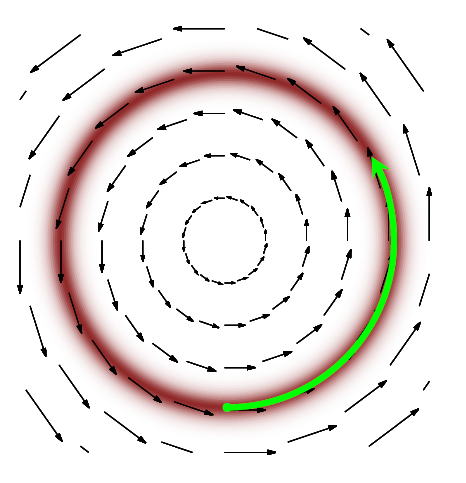
\includegraphics[width=0.4\linewidth]{plot_typical_Set}
     \caption{Plot from \cite{betancourt2017conceptual}. The red band is the typical set. The arrows describe directions aligned with the typical set which guids the sampling algorithm.}\label{fig:typ_set1.1}
\end{figure}

Next, we introduce the momentum parameter $\bm{p}$ which we will use in our calculations but which we marginalise out to recover our target distribution. We lift the target distribution $p(\bm{\theta}) $ onto a joint probability distribution $p_c(\bm{\theta}, \bm{p})$ on the phase space $(\bm{\theta}, \bm{p})$ which we call the canonical distribution. Denoting with $H(\bm{\theta}, \bm{p})$ the invariant Hamiltonian function, the canonical distribution is defined as

\begin{equation}
p_c(\bm{\theta}, \bm{p}) = \exp(-H(\bm{\theta}, \bm{p})).
\end{equation}

Hence, we find that 

\begin{equation}
H(\bm{\theta}, \bm{p}) = -\log(p_c(\bm{\theta}, \bm{p}) ) = -\log(p( \bm{p} |\bm{\theta})) - \log(p(\bm{\theta})) = K(\bm{p}, \bm{\theta}) + V(\bm{\theta}),
\end{equation}

were we use the physical analogy with $K(\bm{p}, \bm{\theta}) = -\log(p( \bm{p} |\bm{\theta}))$ the kinetic energy and $V(\bm{\theta}) = - \log(p(\bm{\theta})) $ the potential energy. Hence, we can use the equations of Hamilton given by

\begin{equation}
\begin{aligned}
\dfrac{d \bm{\theta}}{dt} &= \dfrac{\partial H}{\partial \bm{p}}  \\
\dfrac{d \bm{p}}{dt} &= - \dfrac{\partial H}{\partial \bm{\theta}} .
\end{aligned}
\end{equation}

Hamiltonian systems have some interesting properties like time reversibility and volume preservation in the phase space. In order to solve this system we use symplectic integrators, since they preserve phase space volume. We use the leapfrog integrator which we directly include in the algorithm of HMC. We denote with $\varepsilon$ the step size and with $L$ the length of the Leapfrog integrator. The new state ($\tilde{\bm{\theta}},\tilde{\bm{p})}$, which is the output of the leapfrog, is accepted with probability 

\begin{equation}
\min \left( 1 , \dfrac{p_c(\tilde{\bm{\theta}}, \tilde{\bm{p}}) }{p_c(\bm{\theta}, \bm{p}) } \right) = \min \left( 1 , \dfrac{\exp ( - V(\tilde{\bm{\theta}}) -  K(\tilde{\bm{p}}, \tilde{\bm{\theta}}))  }{\exp ( - V(\bm{\theta}) -  K(\bm{p}, \bm{\theta})) } \right).
\end{equation}

One also needs to choose a kinetic energy function in order to obtain a sample to start our trajectory with. We keep it easy and take 

\begin{equation}
K(\bm{p}, \bm{\theta}) = -\log(p( \bm{p} |\bm{\theta})) = \mathcal{N}(\bm{p}|\bm{0},I) = \dfrac{1}{2}\bm{p}^t \bm{p} + \text{cte}, 
\end{equation}

which we use $M$ times. More possibilities can be found in \cite{betancourt2017conceptual}.  

\begin{figure}[!htb]
     \centering
     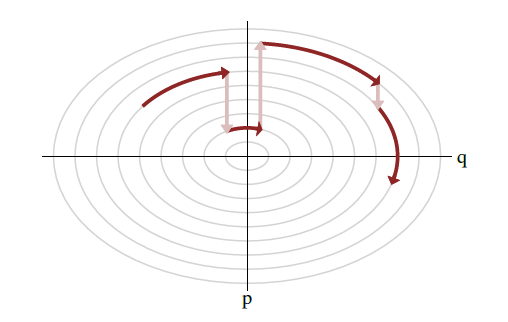
\includegraphics[width=0.4\linewidth]{plot_levelset}
     \caption{Plot from \cite{betancourt2017conceptual}. The pink arrows represent the momentum resampling step and the red arrows the trajectories accros these levels with leapfrog}\label{fig:level_set1.1}
\end{figure}

Before reading algorithm (\ref{MH_algorithm}, figure (\ref{fig:level_set1.1} may be clarifying. Now, the algorithm for Hamiltonian Monte carlo is given by (from \cite{hoffman2014no}). 

\begin{algorithm}
\caption{Hamoltonian Monte Carlo (HMC)}\label{MH_algorithm}
\begin{algorithmic}[1]
\item \textbf{input}: $\bm{\theta}_0, \varepsilon, L, M$
\item \textbf{output}: $\bm{\theta}, \bm{p}$
\BState For \emph{$m = 1, \ldots, M$} do :
\State \quad Sample \emph{$ \bm{p}_0 \sim \mathcal{N}(\bm{p}|\bm{0},I)$}
\State \quad \emph{$\bm{\theta}_{m} = \bm{\theta}_{m-1}, \tilde{\bm{\theta}} = \bm{\theta}_{m-1}, \tilde{\bm{p}} =  \bm{p}_0$}
\State \quad For \emph{$i = 1, \ldots, L$} do:
\State \qquad \emph{$\tilde{\bm{\theta}}, \tilde{\bm{p}} = \text{Leapfrog}(\tilde{\bm{\theta}}, \tilde{\bm{p}}, \varepsilon)$}
\State \quad With probability \emph{$\alpha = \left( 1 , \dfrac{\exp ( \log(p(\tilde{\bm{\theta}}) -\frac{1}{2}\tilde{\bm{p}}^t \tilde{\bm{p}} ) }{\exp ( \log(p(\bm{\theta}_{m-1}) -  \frac{1}{2} \bm{p}_0^t \bm{p}_0 )} \right)$}, set $\bm{\theta}_m = \tilde{\bm{\theta}}$,  $\bm{p}_{m} = -\tilde{\bm{p}}$
\State
\State \textbf{function}: Leapfrog($\bm{\theta},\bm{p}, \varepsilon$)
\State \quad \emph{$\tilde{\bm{p}} = \bm{p} + \dfrac{\varepsilon}{2} \nabla_{\bm{\theta}} \log(p(\bm{\theta})$}
\State \quad \emph{$\tilde{\bm{\theta}} = \bm{\theta} + \varepsilon\tilde{\bm{p}}$ }
\State \quad \emph{$\tilde{\bm{p}} = \tilde{\bm{p}} + \dfrac{\varepsilon}{2} \nabla_{\bm{\theta}} \log(p(\tilde{\bm{\theta}})$}
\State \quad \textbf{return}: $\tilde{\bm{\theta}}, \tilde{\bm{p}}$
\end{algorithmic}
\end{algorithm}

In the proposal, we negated $\tilde{\bm{p}}$ which is necessary to have time reversibility. Notice that this step can be skipped since we are only interested in sampling from $p(\bm{\theta})$. 

Choosing suitable values for $L$ and $\varepsilon$ is very important in order to obtain a good performance. If $L$ is too small, we obtain random walk behaviour and slow mixing. In the opposite case, when $L$ is too large, we generate trajectories that loop back and reiterate the steps. Next, if $\varepsilon$ is too small, we need to do a lot of computations since we need to calculate a new value of the gradient every loop. If $\varepsilon$ is too large, the simulation will be inaccurate and we encounter low acceptance rates. Hence, we use an extension of HMC called the No-U-Turn Sampler (NUTS). 

Interested reader can find the derivation of NUTS in \cite{hoffman2014no}) and some extra plots and explanations in \cite{betancourt2017conceptual}. Without going to technical, NUTS traces out a path forward and backwards in a fictitious time. First, it runs one step backwards or forwards, then two steps backwards or forwards, then four steps backwards or forwards etc. We stop the doubling when the leftmost or rightmost nodes of any balanced subtree of the overall binary tree starts to double back on itself. A tree is balanced if the subtrees are balanced and the height of the subtrees differ by at most one. If the trajectory begins to loop back, it is likely that it retraces its steps and the simulation is wasteful. More rigorously, the doubling process stops if for one of the subtrees the states $\bm{\theta}^{-}, \bm{p}^{-}$ (leftmost leave) and $\bm{\theta}^{+}, \bm{p}^{+}$ (rightmost leave) we have that 

\begin{equation}
(\bm{\theta}^{+} - \bm{\theta}^{-}) \bm{p}^{-} < 0 \quad \text{or} \quad (\bm{\theta}^{+} - \bm{\theta}^{-}) \bm{p}^{+} <0.
\end{equation}

In other words, if an infinitesimal amount forward or backward in time reduces the distance between $\bm{\theta}^{-}$ and $\bm{\theta}^{+}$, we stop. Much more information and extra modifications can be found in the sources. 









%\setcounter{page}{0}
%\pagenumbering{arabic}

%\bibliographystyle{ieeetr}
\bibliographystyle{apalike}
\bibliography{my}

\newpage
% ----------------------- Achterblad ------------------------------
% Vergeet niet de tekst aan te passen:
% - Afdeling
% - Adres van de afdeling
% - Telefoon en faxnummer
% -----------------------------------------------------------------
\thispagestyle{empty}
\sffamily
%
\begin{textblock}{191}(113,-11)
{\color{blueline}\rule{160pt}{5.5pt}}
\end{textblock}
%
\begin{textblock}{191}(168,-11)
{\color{blueline}\rule{5.5pt}{59pt}}
\end{textblock}
%
\begin{textblock}{183}(-24,-11)
\textblockcolour{}
\flushright
\fontsize{7}{7.5}\selectfont
\textbf{DEPARTMENT MATHEMATICS}\\
Celestijnenlaan 200b - bus 2400\\
3001 LEUVEN, BELGI\"{E}\\
tel. + 32 16 32 70 15 \\
fax + 32 16 32 79 98\\
www.kuleuven.be\\
\end{textblock}
%
\begin{textblock}{191}(154,-7)
\textblockcolour{}
\includegraphics*[height=16.5truemm]{sedes}
\end{textblock}
%
\begin{textblock}{191}(-20,235)
{\color{bluetitle}\rule{544pt}{55pt}}
\end{textblock}
\end{document}